\documentclass{nwureport}
\RequirePackage[l2tabu, orthodox]{nag}
\ifx\pdftexversion\undefined
\usepackage[dvips]{graphicx}
\else
\usepackage[pdftex]{graphicx}
% Only print picture outlines...
%\usepackage[pdftex,draft]{graphicx}
\DeclareGraphicsRule{*}{mps}{*}{}
\fi

\usepackage{caption}
\usepackage{siunitx}
\usepackage{pgfgantt}
\usepackage{minitoc}
\usepackage{pdfpages}
\usepackage{dirtree}
\usepackage[toc,page]{appendix}
%\usepackage[a4paper,lmargin=3.0cm, rmargin=1.0cm,tmargin=3.5cm,bmargin=2.50cm]{geometry}

%%%%%%%%%%%%%%%%%%%%%%%%%%%%%%%%%%%%%%%%%%%%%%%%%%%%%%%
% Reset text/figure fractions to more reasonable values
%%%%%%%%%%%%%%%%%%%%%%%%%%%%%%%%%%%%%%%%%%%%%%%%%%%%%%%
\renewcommand{\topfraction}{0.85}
\renewcommand{\textfraction}{0.1}
\renewcommand{\floatpagefraction}{0.79}
%%%%%%%%%%%%%%%%%%%%%%%%%%%%%%%%%%%%%%%%%%%%%%%%%%%%%%%
% Working
%\renewcommand{\topfraction}{0.85}
%\renewcommand{\textfraction}{0.}
%\renewcommand{\floatpagefraction}{0.79}
%%%%%%%%%%%%%%%%%%%%%%%%%%%%%%%%%%%%%%%%%%%%%%%%%%%%%%%

\graphicspath{{./images/}}
\usepackage{longtable}
%\usepackage{fullpage} % reduce margin whitespace
%\usepackage{setspace} % 

% This makes TOC and lists have very little white spacing...
\usepackage{tocloft}
%%%%%%%%%%%%%%%%%%%%%%%%%%%%%%%%%%%%%%%%%%%%%%%%%%%%%%%
% Draft assistance
%%%%%%%%%%%%%%%%%%%%%%%%%%%%%%%%%%%%%%%%%%%%%%%%%%%%%%%
%\usepackage{showkeys}
%\usepackage{showlabels}
%\usepackage{everypage}
%\usepackage{draftwatermark}
%%%%%%%%%%%%%%%%%%%%%%%%%%%%%%%%%%%%%%%%%%%%%%%%%%%%%%%

\usepackage{times} % font

\usepackage{booktabs}

\usepackage{multirow}

\usepackage{cmap}     % to produce searchable PDF

\usepackage{rotating,lscape}

%%%%%%%%%%%%%%%%%%%%%%%%%%%%%%%%%%%%%%%%%%%%%%%%%%%%%%%
% Page style - footers and headers
%%%%%%%%%%%%%%%%%%%%%%%%%%%%%%%%%%%%%%%%%%%%%%%%%%%%%%%
\usepackage{fancyhdr}
\usepackage{tocloft}
\pagestyle{fancy}

\renewcommand{\chaptermark}[1]{\markboth{\thechapter.\ #1}{}} 
\fancyhead{} % clear all header fields

\fancypagestyle{plain}{%
  \renewcommand{\headrulewidth}{0pt}% Header rule thickness
  \renewcommand{\footrulewidth}{0pt}% Footer rule thickness
  \fancyhf{}% Clear header/footer
  \fancyhead[L]{}% Chapter in header Left
  \renewcommand{\headrulewidth}{\iffloatpage{0pt}{0pt}}
  \fancyfoot[C]{-\thepage-} % Page number at the bottom 
}
%\fancypagestyle{frontmatter}{%
%  \renewcommand{\headrulewidth}{0pt}% No header rule
%  \renewcommand{\footrulewidth}{0pt}% No footer rule
%  \fancyhf{}% Clear header/footer
%  \fancyfoot[C]{-\thepage-}%
%}
\fancypagestyle{mainmatter}{%
  \renewcommand{\headrulewidth}{0pt}% Header rule
  \renewcommand{\footrulewidth}{0pt}% Footer rule
  \fancyhf{}% Clear header/footer
%  \fancyhead[L]{\scshape\leftmark}% Chapter in header Left
  \fancyhead[R]{Assessing the source contribution to atmospheric particulate matter in Wedela}% Page number in header Right
  \renewcommand{\headrulewidth}{\iffloatpage{0pt}{0pt}}
  \fancyfoot[C]{-\thepage-} % Page number at the bottom 
}

%doesn't work
%%\addtolength{\headheight}{5pt} 
%%\cfoot[]{-\thepage-}
%\fancyfoot{} % clear all footer fields
%\fancyfoot[C]{-\thepage-}
%%\renewcommand{\headrulewidth}{0pt}
%%\renewcommand{\footrulewidth}{0pt}

%%%%%%%%%%%%%%%%%%%%%%%%%%%%%%%%%%%%%%%%%%%%%%%%%%%%%%%

\usepackage[section]{placeins}

\usepackage{amsmath,url}
\usepackage{subeqnarray}

%pdfpagelabels, % Need to solve the figure count reset to use this
%%%%%%%%%%%%%%%%%%%%%%%%%%%%%%%%%%%%%%%%%%%%%%%%%%%%%%%%%%%%%
% Hyperref pdf options
%%%%%%%%%%%%%%%%%%%%%%%%%%%%%%%%%%%%%%%%%%%%%%%%%%%%%%%%%%%%%
\usepackage[pdftitle={Assessing the source contribution to atmospheric particulate matter in Wedela},pdfpagemode=UseOutlines,colorlinks,pdfauthor={Roelof
    Burger},bookmarks=true,pdftex=true,hyperindex,plainpages=false,pdfpagelabels,pagebackref]{hyperref}
%\hypersetup{colorlinks,linkcolor=black,citecolor=black,pdfstartview=Fit}
\hypersetup{pdfstartview=Fit}
%%%%%%%%%%%%%%%%%%%%%%%%%%%%%%%%%%%%%%%%%%%%%%%%%%%%%%%%%%%%%

%%%%%%%%%%%%%%%%%%%%%%%%%%%%%%%%%%%%%%%%%%%%%%%%%%%%%%%%%%%%%
% TOC font settings
%%%%%%%%%%%%%%%%%%%%%%%%%%%%%%%%%%%%%%%%%%%%%%%%%%%%%%%%%%%%%
%\usepackage[titles]{tocloft}
%\renewcommand{\cfttoctitlefont}{\sffamily}
%%%%%%%%%%%%%%%%%%%%%%%%%%%%%%%%%%%%%%%%%%%%%%%%%%%%%%%%%%%%%
% Advanced glossaries package
%%%%%%%%%%%%%%%%%%%%%%%%%%%%%%%%%%%%%%%%%%%%%%%%%%%%%%%%%%%%%
\usepackage[toc,style=long]{glossaries}
%%%%%%%%%%%%%%%%%%%%%%%%%%%%%%%%%%%%%%%%%%%%%%%%%%%%%%%%%%%%%

\usepackage{enumerate}
\usepackage{verbatim}  %  This is to use \begin{comment} ...

%\usepackage{sectsty}
%\allsectionsfont{\usefont{OT1}{phv}{bc}{n}\selectfont}
%\usepackage[sf]{titlesec}


%%%%%%%%%%%%%%%%%%%%%%%%%%%%%%%%%%%%%%%%%%%%%%%%%%%%%%%%%%%%%
% Glossaries and abbreviations
%%%%%%%%%%%%%%%%%%%%%%%%%%%%%%%%%%%%%%%%%%%%%%%%%%%%%%%%%%%%%
\usepackage[toc,style=long]{glossaries}

\newglossary{abbreviation}{aot}{ata}{Abbreviations}
%\newglossary{compounds}{cot}{cts}{List of Compounds}
% \newglossary{symbols}{sot}{sts}{List of Symbols}
\loadglsentries[abbreviation]{abbreviations}
%\loadglsentries[compounds]{compounds}
% \loadglsentries[symbols]{symbols}
\makeglossaries
%%%%%%%%%%%%%%%%%%%%%%%%%%%%%%%%%%%%%%%%%%%%%%%%%%%%%%%%%%%%%

\usepackage{natbib}
\begin{document}
\bibliographystyle{crg}

     \title{Asessing the source contribution to atmospheric particulate matter in Wedela}
     %\title{The establishment of rain gauge networks for rainfall estimation calibration of the South African new weather network}
     \author{
        Roelof Burger
          \thanks{
             Climatology Research Group\\
             Unit for Environmental Sciences and Management \\
             North-West University, Potchefstroom, 2520, South Africa \\
             {\tt roelof.burger@nwu.ac.za}} \\
        Henno Havenga
          \thanks{
             Climatology Research Group\\
             Unit for Environmental Sciences and Management \\
             North-West University, Potchefstroom, 2520, South Africa \\
             {\tt hhavenga92@gmail.com}} \\
        Stuart Piketh
          \thanks{
             Climatology Research Group\\
             Unit for Environmental Sciences and Management \\
             North-West University, Potchefstroom, 2520, South Africa \\
             {\tt stuart.piketh@nwu.ac.za}} \\
     }
     \activity{Progress report}
     \projnumber{WEDANG01-QR1v1}
     \lab{Environmental Sciences and Management}
     \keywords{air quality, low-income settlements, townships, winter}
     \maketitle

\pagenumbering{roman}

\chapter*{Executive Summary}

\pagebreak

\chapter*{Acknowledgments}

The data was collected and analysed by:
\\
\begin{tabular}{ l l } 
Joe Malahlela  & NWU \\
Thomas Bigala  & NWU \\
Roelof Burger  & NWU \\
Marvin Qhekwana & NWU \\
Thapelo Letsolo & NWU \\
Brigitte Language & NWU \\
Kealeboga Ntshabele & NWU \\
\end{tabular}

\clearpage

\dominitoc
\setcounter{tocdepth}{2} % set depth level of TOC
\pagestyle{plain}
{\thispagestyle{plain}
\tableofcontents
% Add page heading 
\addtocontents{toc}{~\hfill\textbf{Page}\par}
\addcontentsline{toc}{chapter}{Contents}
\clearpage
\listoffigures
\addtocontents{lof}{~\hfill\textbf{Page}\par}
\addcontentsline{toc}{chapter}{Figures}
\clearpage
\listoftables
\addtocontents{lot}{~\hfill\textbf{Page}\par}
\addcontentsline{toc}{chapter}{Tables}
%\clearpage
\printglossaries
%\clearpage
}

\pagenumbering{arabic}
\pagestyle{mainmatter}

%%%%%%%%%%%%%%%%%%%%%%%%%%%%%%%%%%%%%%%%%%%%%%%%%%%%%%%%%%%%%

\chapter{Introduction}

The association between air pollutants and health are well established (Dockery, 1993; Poppe et al., 2002). The strongest link

Katsouyanni et al., 2001, Samet et al. 2000, Atkinson et al, 2014.

Evidence 

This report describes the 

Air quality related health impacts represents the greatest environmental health impact (Lim et al, 2012).
Numerous sources contribute to ambient air quality levels. The relative contribution of different sources also
vary significanly in space and time. Particulate matter is the most significant cause of human health impacts
from poor air quality in South Africa currently. The total atmospheric loading of PM is associated with a
diverse set of sources. In the context of the South African Highveld these could include agricultural activities;
domestic fuel burning; opencast mining; power generation; refuge burning; wind-blown dust or motor vehicle
emissions. Recent studies confirm that the biggest air pollution problems in South Africa are find in the area
of low-income settlements (Hersey et al 2015). These areas are typically exposed to a multitude of low-level
local sources in close proximity to where people spend most of their time. In order to implement an effective
strategy to reduce ambient PM levels it is important to understand which of the sources listed above
contribute the most to poor air quality. Low-income areas have the worst ambient air quality. These areas
further holds great significance, as it is also home to a large proportion of South Africans. In this project an
attempt will be made to apportion the contributions of identified sources to the ambient PM loading in the
Wadela Township in Gauteng. The specific objectives of this project can be summarised as:

\begin{itemize}
\item Determine the ambient particulate loading at one ambient air quality site in the Wadela township;
\item Determine the temporal variation of aerosol loading in Wadela;
\item Characterize the chemical composition of the aerosol samples at the Wadela ambient monitoring station;
\item Apportion the sampled ambient particulate loading in Wadela to the contributing sources.
\end{itemize}

%\minitoc

%%%%%%%%%%%%%%%%%%%%%%%%%%%%%%%%%%%%%%%%%%%%%%%%%%%%%%%%%%%%%
\begin{figure}[!htb]
\definecolor{barblue}{RGB}{153,204,254}
\definecolor{groupblue}{RGB}{51,102,254}
\definecolor{linkred}{RGB}{165,0,33}
\renewcommand\sfdefault{phv}
\renewcommand\mddefault{mc}
\renewcommand\bfdefault{bc}
\setganttlinklabel{s-s}{START-TO-START}
\setganttlinklabel{f-s}{FINISH-TO-START}
\setganttlinklabel{f-f}{FINISH-TO-FINISH}
\sffamily
\begin{ganttchart}[
canvas/.append style={fill=none, draw=black!5, line width=.75pt},
hgrid style/.style={draw=black!5, line width=.75pt},
vgrid={*1{draw=black!5, line width=.75pt}},
today=7,
today rule/.style={
draw=black!64,
dash pattern=on 3.5pt off 4.5pt,
line width=1.5pt
},
today label font=\small\bfseries,
title/.style={draw=none, fill=none},
title label font=\bfseries\footnotesize,
title label node/.append style={below=7pt},
include title in canvas=false,
bar label font=\mdseries\small\color{black!70},
bar label node/.append style={left=2cm},
bar/.append style={draw=none, fill=black!63},
bar incomplete/.append style={fill=barblue},
bar progress label font=\mdseries\footnotesize\color{black!70},
group incomplete/.append style={fill=groupblue},
group left shift=0,
group right shift=0,
group height=.5,
group peaks tip position=0,
group label node/.append style={left=.6cm},
group progress label font=\bfseries\small,
link/.style={-latex, line width=1.5pt, linkred},
link label font=\scriptsize\bfseries,
link label node/.append style={below left=-2pt and 0pt}
]{1}{13}

\gantttitle[title label node/.append style={below left=7pt and -3pt}]{Months:\quad1}{1}

\gantttitlelist{2,4,...,24}{1} \\

\ganttgroup[progress=57]{WBS 1 Ambient monitoring}{1}{12} \\
\ganttbar[progress=75, name=WBS1A]{\textbf{WBS 1.1} Site installation}{1}{2} \\
\ganttbar[progress=67, name=WBS1B]{\textbf{WBS 1.2} Ambient PM2.5}{2}{12} \\
\ganttbar[progress=60, name=WBS1C]{\textbf{WBS 1.3} Ambient PM10}{2}{12} \\
\ganttbar[progress=60, name=WBS1D]{\textbf{WBS 1.4} Ambient meteorology}{1}{12} \\[grid]

\ganttgroup[progress=65]{WBS 2 Source apportionment}{3}{9} \\
\ganttbar[progress=70]{\textbf{WBS 2.1} 4 field campaigns}{4}{5} \\
\ganttbar[progress=50]{\textbf{WBS 2.2} Elemental analysis}{6}{8} \\
\ganttbar[progress=25]{\textbf{WBS 2.3} Anion/Cation analysis}{9}{10} \\[grid]
\ganttbar[progress=10]{\textbf{WBS 2.4} Receptor modelling}{9}{10} \\[grid]

\ganttgroup[progress=100]{WBS 3 Student participation}{1}{13} \\
\ganttbar[progress=90]{\textbf{WBS 3.1} Marvin Qhekwana}{1}{8} \\
\ganttbar[progress=90]{\textbf{WBS 3.2} Thapelo Letsholo}{1}{8} \\
\ganttbar[progress=10]{\textbf{WBS 3.3} Kealeboga Ntshabela}{6}{13} \\
\ganttbar[progress=0]{\textbf{WBS 3.4} Prince Chidhindi}{6}{13} \\[grid]

\ganttgroup[progress=5]{WBS 4 Dispersion modelling}{7}{12} \\
\ganttbar[progress=75, name=WBS1A]{\textbf{WBS 1.1} Emissions inventory}{7}{9} \\
\ganttbar[progress=67, name=WBS1B]{\textbf{WBS 1.2} Meteorological analysis}{7}{9} \\
\ganttbar[progress=50, name=WBS1C]{\textbf{WBS 1.3} Modelling}{6}{10} \\
\ganttbar[progress=20, name=WBS1D]{\textbf{WBS 1.4} Reporting}{10}{12} \\[grid]
\end{ganttchart}
\end{figure}


\chapter{Proposed methodology}

Different approaches are used to apportion the contribution of sources to ambient particular matter. The most
common technique is to estimate source emissions and then model the resultant ambient concentrations.
Uncertainties in emission estimates, meteorological variability and model imprecisions have to be overcome
to for this to yield reliable information. Receptor model represents the inverse method, where detailed
measurements at a particular point are used to estimate the contribution of different sources using their
chemical footprint. While this is only represented for the time and place of the measurements, it can be used
to inform other efforts to quantify and prioritize source contribution.

\section{Determine the loading and temporal variation of ambient particulate matter in Wadela}

Ambient measurements of particulate matter provides the core justification for the study. It confirms the state
of ambient air quality and confirms the rationale for the project. It further serves to put the source
apportionment filter samples into the broader context. Continues measurements of particulate matter smaller
than 2.5 micron (PM2.5) and smaller than 10 micron (PM10) will be measured for a 24 month period.

\section{Characterizing the chemical composition of ambient particulate matter in Wadela}

Samples will be collected for a two week period during winter and summer. Two samples a day will split the
typical bimodal ambient concentration peaks observed in low income communities in other regions. Sampling
will be undertaken using a Stacked Filter Unit (SFU) sampler. The sampler collects particles which have an
equivalent aerodynamic diameter (EAD) of less than 10 μm in separate coarse and fine fractions. The
coarse fraction corresponds to aerosols collected with an EAD between 10 and 2.5 μm while the fine fraction
corresponds to aerosols collected with an EAD lower than 2.5 μm. Two 47-mm Nucelopore polycarbonate
filters with diameters of 8.0 μm and 0.4 μm were sequentially used during sampling.
After sampling, the nucleopore filters are stabilised 24 hours prior to weighing and then placed in a stabilised
environment prior to energy dispersive X-Ray Fluorescence (XRF) and Ion Chromatography (IC) Analysis.
The extracts are analysed with a Metrohm 850 Professional IC. The Chromatograph has a Metrosep A Supp
15 Anion Membrane and a Metrosep C 4 250 Cation Membrane. The IC analysis will be performed for the
following anions and cations, F - , Cl - , Br - , NO 3- , SO 42- , PO 43- , Na + , NH 4+ , K + , Ca + , Mg + .All these procedures are conducted in a stabilized room to prevent any contamination. The results of particle
composition analyses are necessary for identifying all the polluting sources that contributed to the collected
samples (Begum et al, 2007). Source profiles obtained along with the chemical data for receptor samples
are then constructed from literature.

\section{Apportion the contributing sources to the sampled ambient particulate loading in Wadela}

The chemical species present in atmospheric particulates reveals their sources. Geological material contains
large abundances of Al, Si, K, Ca and Fe. . WHile abundances of Al, K, Ca and Fe are similar among the
source profiles in unpaved and paved road dust. Elemental carbon abundances are highly variable in
geological material and are often negligible in natural soil samples while organic carbon is 5 – 15% in
geological profiles, being most abundant in paved road dust and agricultural dust. Motor vehicle emissions
are likely contributors to Pb, EC and OC abundances observed in paved road dust. In general, abundances
of SO 42- , NO 3- and NH 4+ are low, falling in the range of \SIrange{0}{0.3}{\percent}. Na and Cl are also low, with less than \SI{0.5}{\percent}
in abundance. Elemental and organic carbon are the most abundant species in motor vehicle exhaust,
contributing to over 95\% of the total mass. However, Pb and Br abundances are low and highly variable. Zn
was found in most vehicle exhaust profiles, although present at low abundance (0.05\% or less) (Watson et
al., 2004). Fine fraction particulate profiles undertaken by Watson et al (1996) for residential wood
combustion, residential coal combustion and forest fires found average organic carbon abundances to range
from approximately 50\% in residential wood combustion and forest fire profiles to approximately 70\% in the
residential coal combustion profiles. Elemental carbon profiles averaged 3\%, 12\% and 26\% in forest fires,
residential wood combustion and residential coal combustion profiles, respectively. The organic carbon/total
carbon ratio was highest in the forest fire profile with a ratio of 0.94. Similar ratios were observed for
residential wood and coal combustion profiles, with 0.81 and 0.73 recorded, respectively (Watson et al.,
2004). Calloway et al (1989) found K + /K ratios of 0.80 to 0.90 in burning profiles compared to the low ratios
measured in geological material. SO 42- , NO 3- and Si abundances in residential coal combustion are 2 – 4
times higher than those in residential wood combustion and forest fire profiles.
Profiles for coal fired power generation differ substantially from residential coal combustion, despite the fuels
being similar, due to the different emission control technologies used. SO 42- has very high abundances in the
particle phase while SO 2 can be hundreds to thousands times higher than the particle mass. Crustal
elements such as Si, Ca and Fe in the coal-fired power generation profiles are present at 30 – 50\% of the
corresponding levels found in the geological material. Al is present at similar or higher levels in the power
generation profile as compared to the geological material. Other elements such as P, K, Ti, Cr, Mn, Sr, Zr and
Ba have less than 1\% abundances. Se has also been detected at abundances of 0.2 – 0.4\% in coal fired
power station emissions which does not have scrubbers installed (Watson et al., 1996). Abundances of
SO 42- , NO 3- and NH 4+ in directly emitted particles cannot account for the concentration of the species
measured in the atmosphere as ambient concentrations contain both primary and secondary particles. SO 2 ,
NH 4 and NO x are the precursors for sulfuric acid, ammonium bisulfate, ammonium sulfate, and ammonium
nitrate particles (Seinfeld, 1986; Watson et al., 1994). Several VOCs may also change into particles due to
photochemical transformation (Grosjean and Seinfeld, 1989). Several of these particles, notably those
containing ammonium nitrate, are volatile and transfer mass between the gas and particle phase to maintain
a chemical equilibrium (Stelson and Seinfeld, 1982a-c). This volatility has implications for ambient
concentration measurements as well as for gas and particle concentrations in the atmosphere.
Once the samples had been analysed, statistical receptor models were then applied to the aerosol data for
source apportionment purposes. Receptor modelling is used to characterise particulate air pollutant sources
and calculate each source contribution to a particular pollutant. There are two main techniques based on
chemical mass balance and multivariate statistics. Chemical Mass Balance (CMB) uses both known profiles
of source emissions and ambient data from the measuring site while multivariate methods can only identify
sources from ambient measurements (Harrison and Yin, 2004). These models have been widely used for
aerosol source apportionment studies.

Principal Components Analysis (PCA) is a statistical factor analysis method based on the law of conservation
of mass. It operates by first extracting a series of principal factors (components) from the measured data on
pollutant concentrations, on the basis of the mutual correlation between the different species. These are
then interpreted as putative sources, and the contribution from each estimated from the factor scores.
PCA is a multivariate modelling technique that does not need data on source compositions as inputs. It can
therefore be used to identify sources, and estimate contributions, where detailed information on source
characteristics is not available, but where a substantial amount of measured concentration data exists.
PCA is based on the analysis of the correlation between measured concentrations of chemical species in a
number of samples, assuming that highly correlated compounds come from the same source. The method
can thus be used to detect the hidden source information from ambient measurement datasets. Ambiguitiesinevitably arise during interpretation of the factors, and the validity of the interpretation depends on good
prior understanding of possible source characteristics; in the absence of such knowledge the results
obtained can thus be somewhat hypothetical and tentative.

PCA assumes that the composition of the emission sources is constant over the sampling period at the
receptors; chemical species do not interact with each other and their concentrations are linearly additive;
source profiles are linearly independent of each other; measurement errors are random and uncorrelated;
the number of species is greater than or equal to the number of sources; the number of samples is much
greater than the number of source types to ensure statistically meaningful calculations; variability of the
concentrations from sample to sample is primarily due to differences in source contribution and not due to
measurement uncertainty or changes in source composition; and the effect of processes that affect all
sources equally (e.g. atmospheric dispersion) is much smaller than the effect of processes that influence
individual sources (e.g. wind direction and changes in emission rates).

Chemical mass balance receptor models are used to apportion measured pollutant concentrations (or
exposures or doses) to their sources, and to assess the proportional contribution of each source. Chemical
mass balance models combine the chemical and physical characteristics of gases and particles measured at
the sources and receptors to both identify the presence of and to quantify source contributions to receptor
concentrations (Schauer et al., 2005). The CMB receptor model was first applied by Winchester and Nifong
(1971), Hidy and Friedlander (1972), and Kneip et al (1973). The original applications used unique chemical
species associated with each source-type, the so-called “tracer” solution. Friedlander (1973) introduced the
ordinary weighted least-squares solution to the CMB equations which had the advantages of relaxing the
constraint of a unique species in each source-type and of providing estimates of uncertainties associated
with the source contributions. Gordon (1980, 1988) and Kowalkzyk et al (1978) subsequently applied this
method to elemental concentrations measured in source and receptor samples. However, the ordinary
weighted least squares solution was limited in that only the uncertainties of the receptor concentrations were
considered while the uncertainties of the source profiles, which were usually much higher than the
uncertainties of the receptor concentrations, were not considered (Coulter, 2004). The ambient chemical
concentrations are expressed as the sum of the products of species abundances and source
contributions. The equations are solved for source contributions, using the ambient concentrations and
source profiles as inputs. CMB models can be applied when the measured ambient concentration of different
species (Cij ) and the number of sources and their profiles (p and fpj) are known. The mass contribution
from each source to each sample (g ip ) is found by a least squares solution of the over determined system of
equations.

The CMB model provides information on which combinations of profiles are likely to provide contributors by
means of statistical performance measures (Watson et al., 1991). The important measures that are
evaluated for each sample are: 1) the source contributions estimates and their uncertainties, 2) ‘chi-square’,
the weighted sum of the squares of the differences between calculated and measures species
concentrations (values between two and four indicate acceptable fits while values less than one indicate
good fits to the data), 3) ‘r-square’, the fraction of the variance in the measured concentrations accounted for
by the variance in the calculated species concentrations (values greater than 0.9 indicate a good fit to the
measured data) and 4) ‘percent mass’ or the percent of the total mass accounted for by the source
contribution estimates (values of between 80 – 120\% are considered to be good) (Kuhns et al., 2002).
The CMB output also contains the ratios of calculated to measured concentration (C/M) and the ratio of the
difference between calculated and measured concentration divided by the uncertainty of this difference (R/U)
for each chemical species. These ratios are indicative of the fits of the individual species (Kuhns et al.,
2002). The ‘Eligible Space Dimension and Maximum Uncertainty’ clusters identify collinearity of similarity
between source profiles. This treatment (Henry, 1992) uses two parameters, maximum source uncertainty
and minimum source projection on the eligible space. The maximum source uncertainty determines the
eligible space to be spanned by the eigenvectors whose inverse singular values are less than or equal to the
maximum source uncertainty. The ‘Number of Estimable Sources’ are the source contributions that are
estimable given their source contributions and propagated uncertainties. Collinearity may result from small
source contribution estimates with relatively large uncertainties. The appearance of profiles in the eligible
space clusters does not invalidate the source contribution estimates. These clusters offer guidance that the
relative uncertainties of the source contribution estimates might be reduced by eliminating one or more of the
profiles or by linearly combining the profiles into a new profile that represents the combined contribution from
both source types (Kuhns et al., 2002).

The CMB model assumes that all sources contributing significantly to measured concentrations are identified
and their emission source profiles are characterized; source profiles are constant over the receptor andsource sampling period; species included are not reactive (i.e. they add linearly); the number of sources or
source categories is less than the number of chemical species; source profiles are linearly independent of
each other and measurement uncertainties are random, uncorrelated and normally distributed (Coulter,
2004).

However, these assumptions are a limitation of the model as source compositions are not constant;
components do react with each other and systems are not linear; it is generally not known how many
sources are contributing to a receptor; there are more sources than components which can be practically
measured; many sources have very similar compositions; measurement errors are not necessarily random,
uncorrelated or normally distributed and few sources have their own unique tracer components (Watson,
1984).

\section{Site description}
Wedela is a small, low income settlement located in the Gauteng province of
South-Africa (26°27'58"S 27°23'0"E). The settlement is in close proximity to Carltonville
and also less than 80km from Johannesburg, the area is also known for the various goldmines
that operate in the area. \hyperref[fig:wadela]{Figure \ref{fig:wadela}}
indicates the relative position of Wedela in South-Africa and in proximity to other major
in the region.

\begin{figure}[!htb]
    \centering
    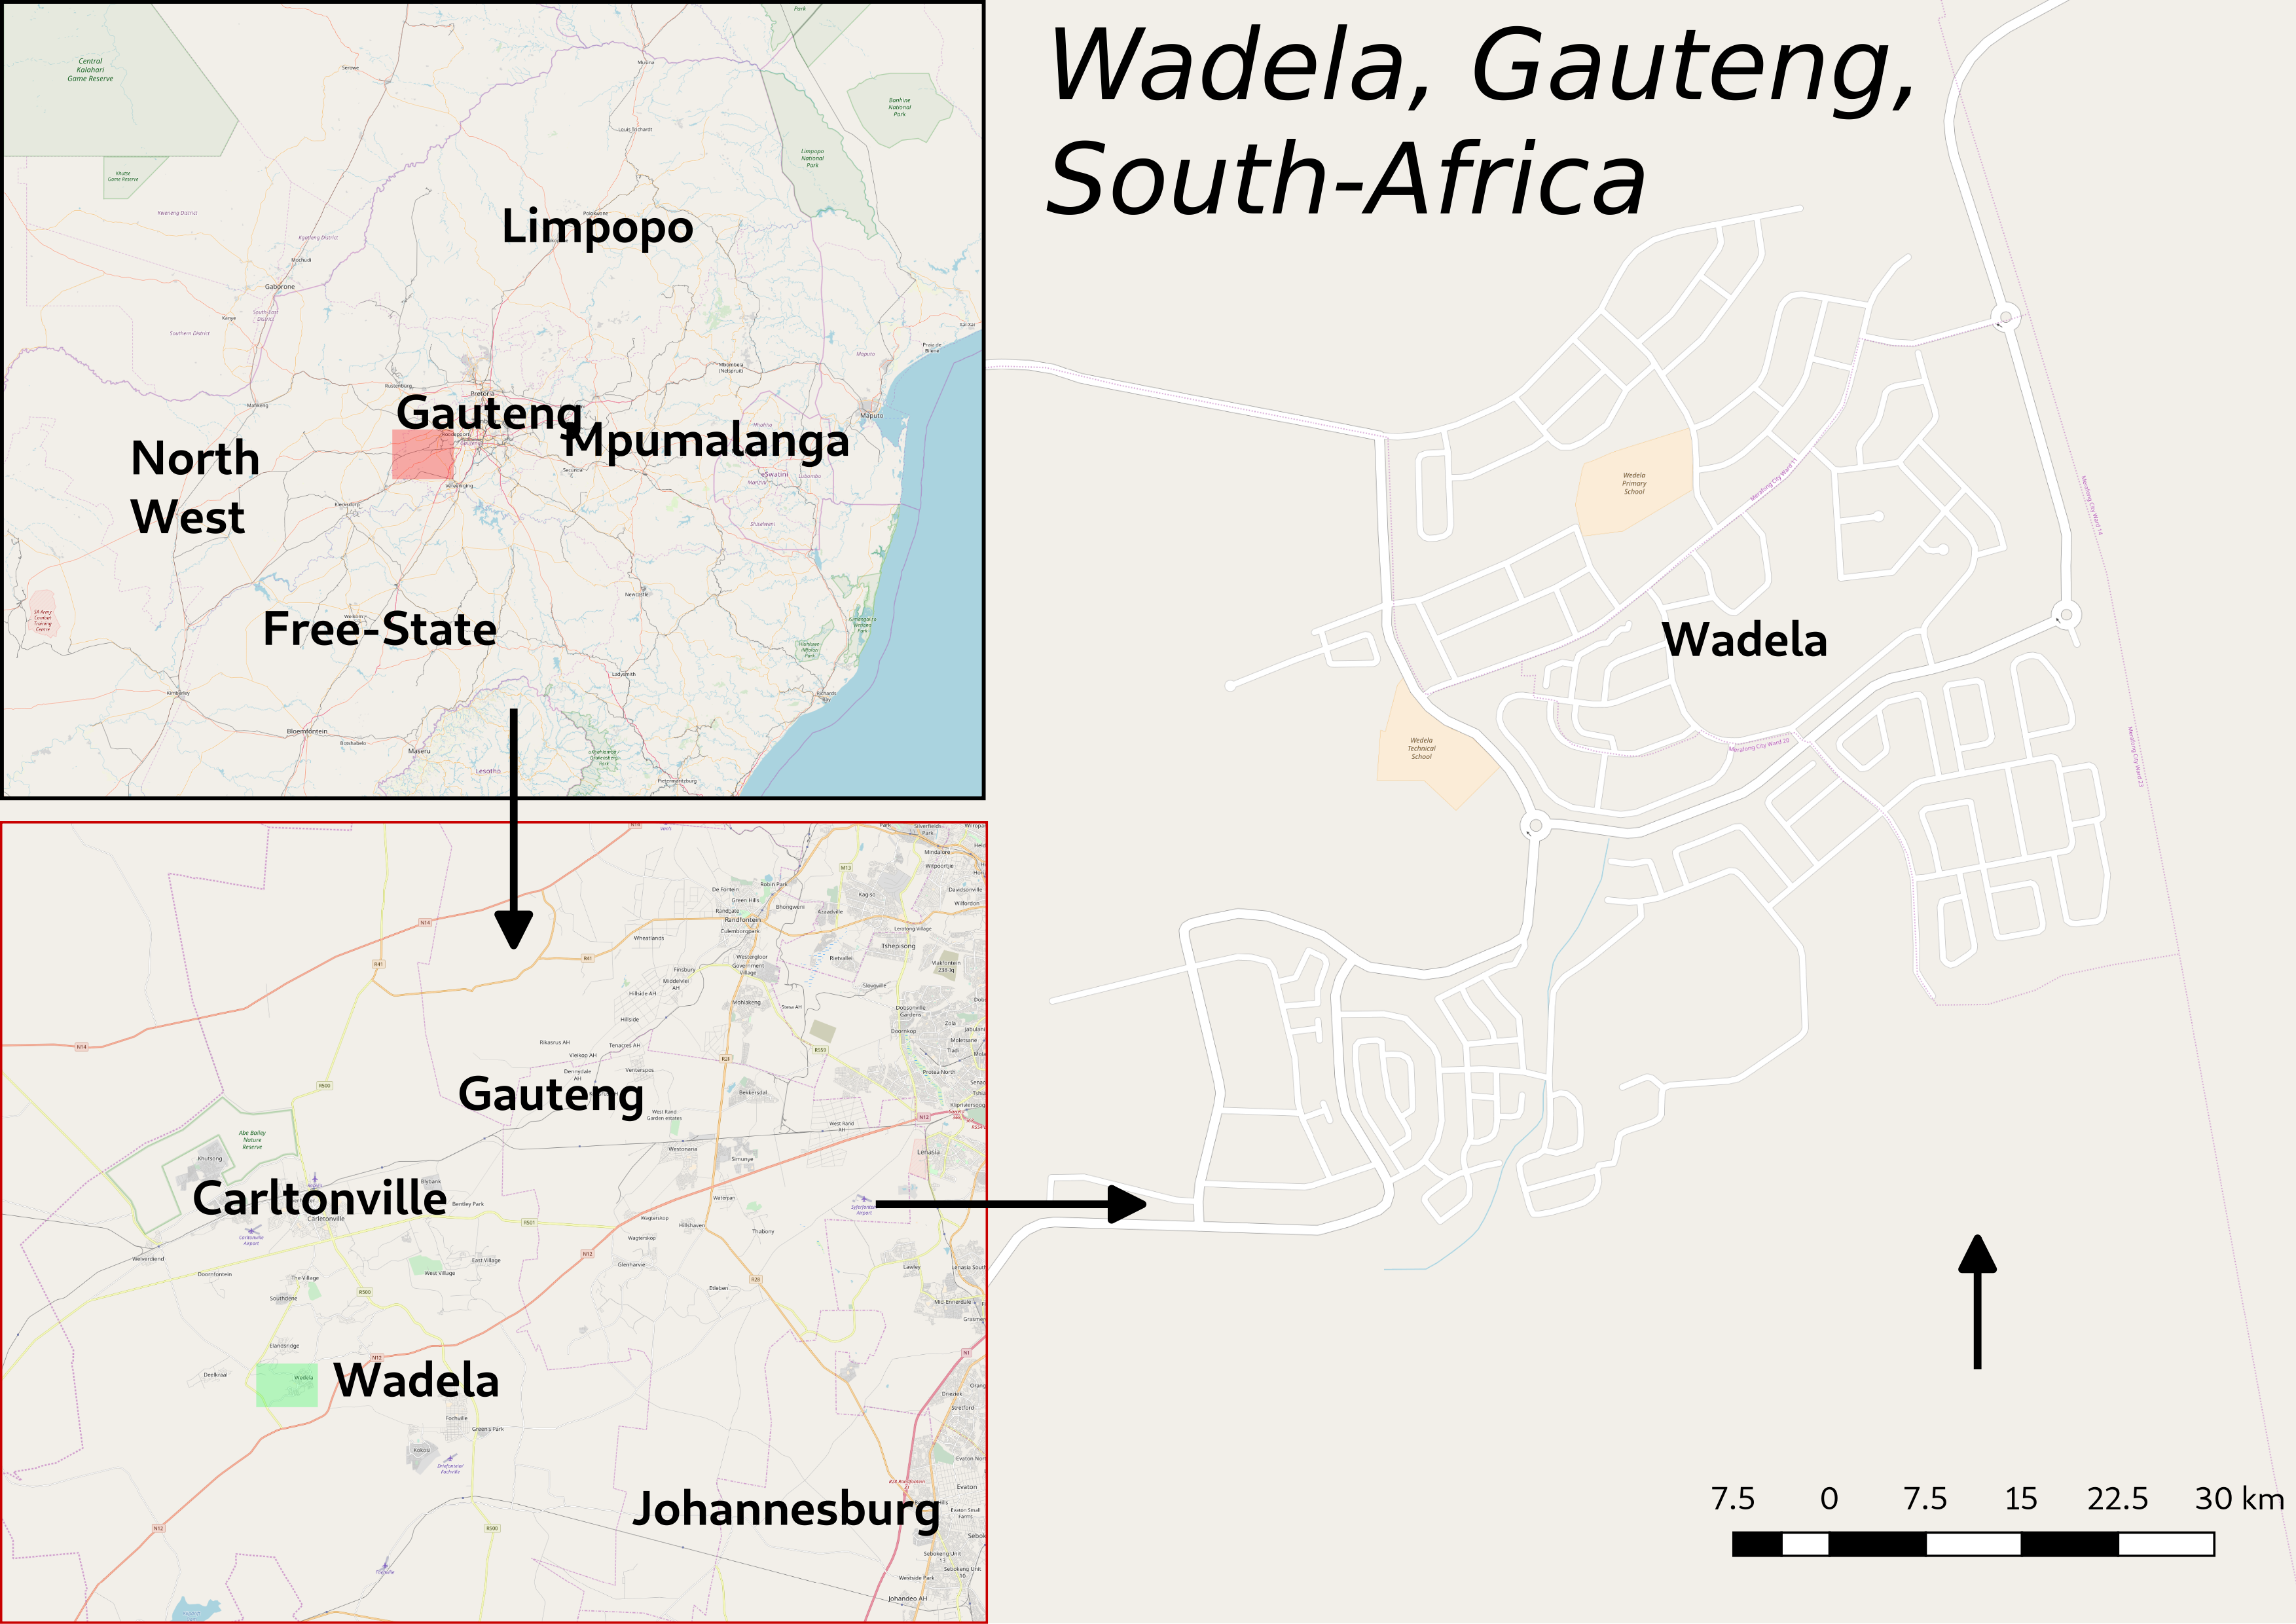
\includegraphics[width=\textwidth]{images/study_area_qgis.png}
    \caption[Study area: Wedela, Gauteng]{Wedela, seen in the above map, is the location where
    the study was conducted. The settlement is located in close proximity to Carltonville and Johannesburg.
    There is also various gold mines present in the region. The map shows Wedela's relative position in
    South-Africa as indicated in the overlay maps.}
    \label{fig:wadela}
\end{figure}


\section{Characterizing ambient particulate matter}
Two EBAMs, one PM10 and one PM2.5 

Talk to Lucky, survey, source profiles

\subsection{Instruments}


\begin{figure}[!htb]
    \centering
    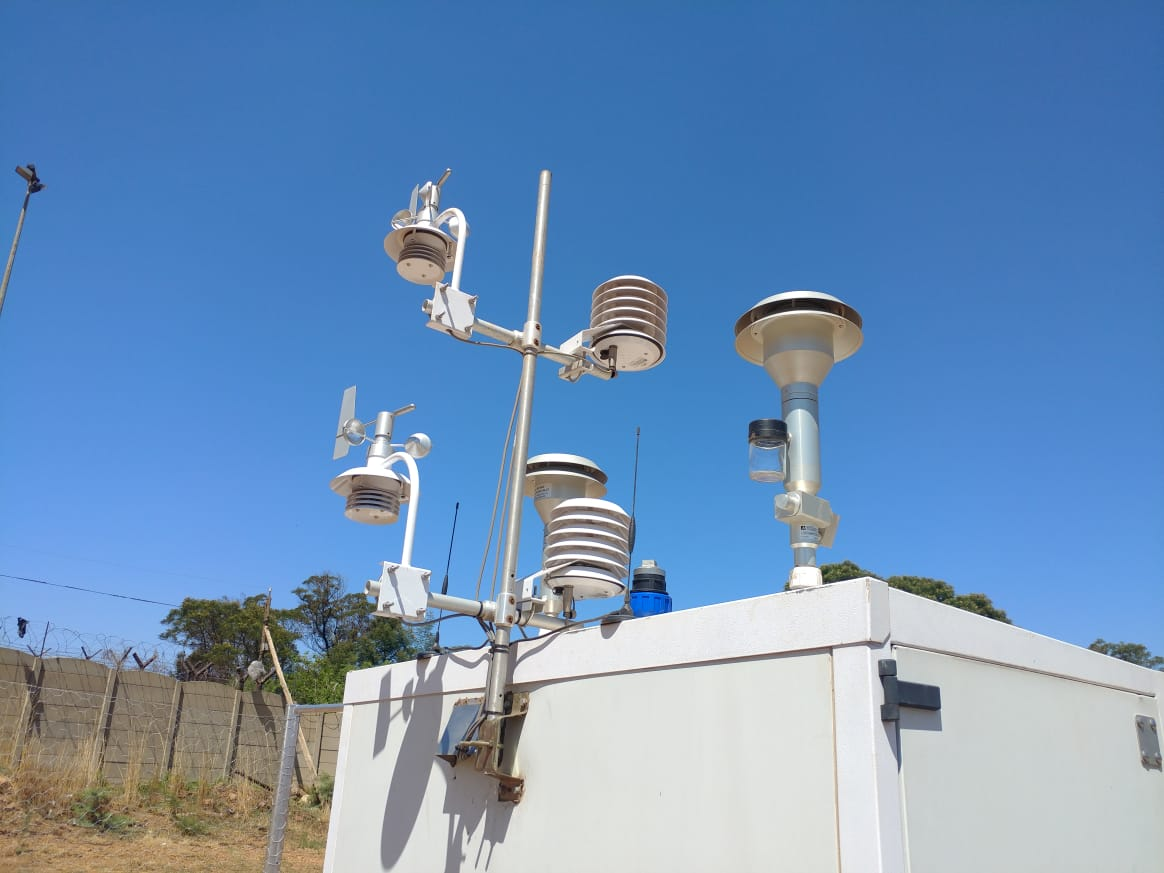
\includegraphics[width=\textwidth]{images/wedela.jpeg}
    \caption[]{Caption}
    \label{fig:wadela_instruments_met}
\end{figure}

\begin{figure}[!htb]
    \centering
    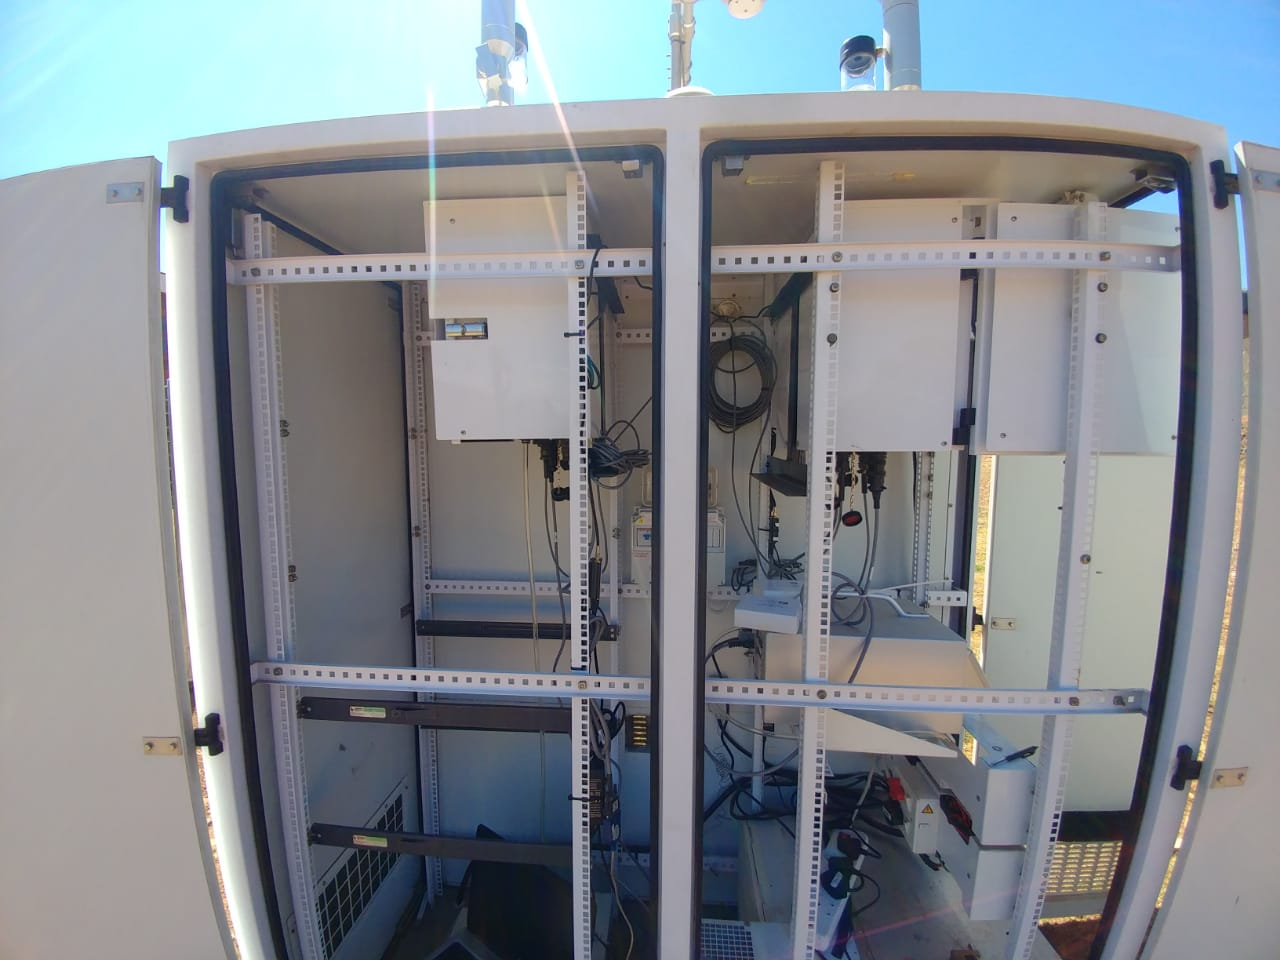
\includegraphics[width=\textwidth]{images/wadela_10.jpeg}
    \caption[]{Caption}
    \label{fig:wadela_instruments_pm}
\end{figure}

\begin{figure}[!htb]
    \centering
    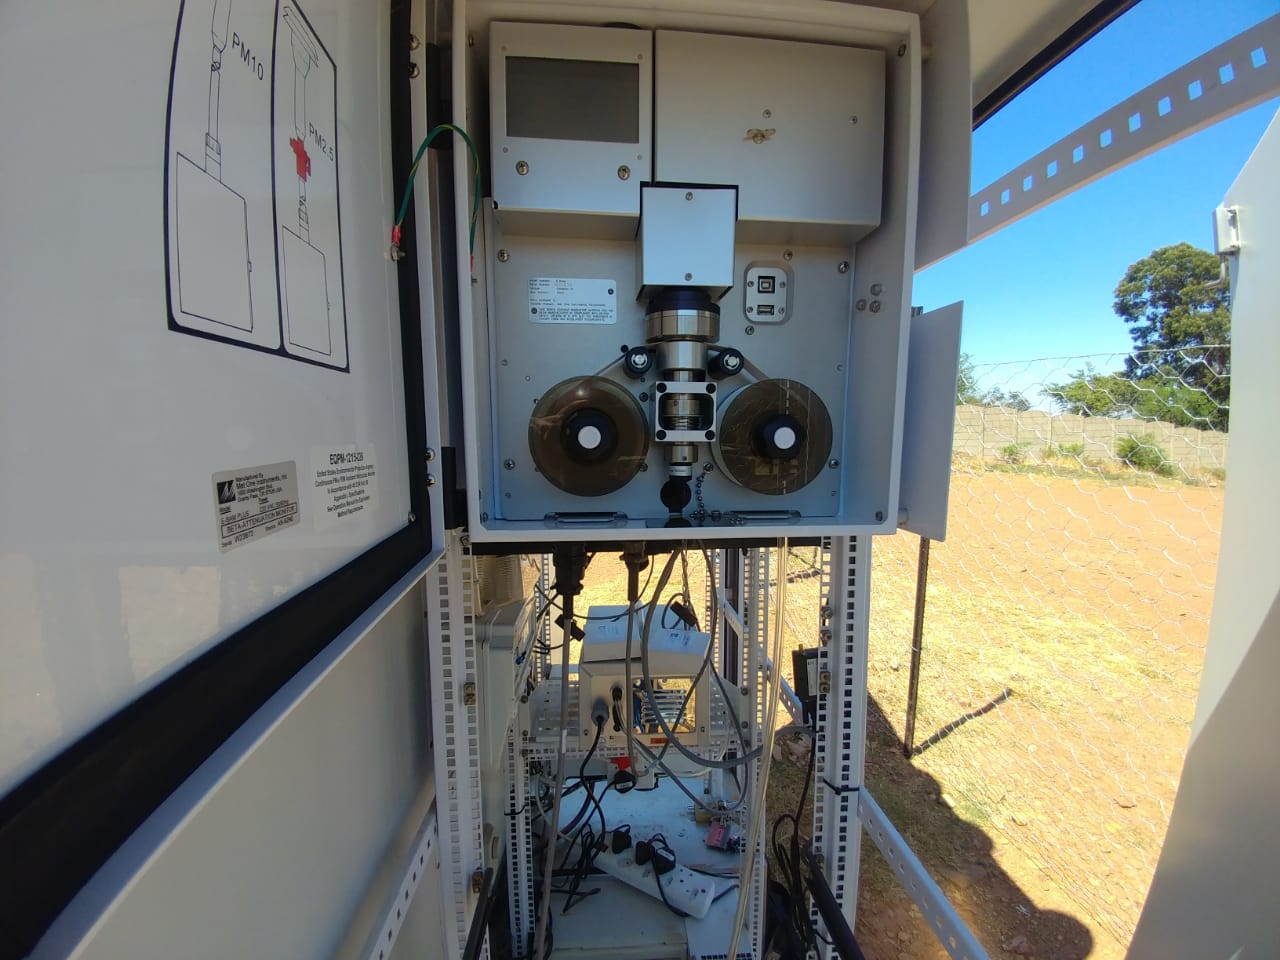
\includegraphics[width=\textwidth]{images/wedela_6.jpeg}
    \caption[]{Caption}
    \label{fig:wadela_instruments_pm2}
\end{figure}

\section{Characterizing sources of particulate matter}

\section{Characterizing sources contribution}

Source apportionment methodology

\section{Modelling ambient concentrations}

Dispersion modelling using AERMOD

\section{Realtime data access}

A real-time monitoring solution has been established through \url{www.ecostat.co.za} to
the EBAM PM2.5 and PM10 instruments located in Wadela. Ecostat allows users to access the data
through any browser such as Firefox, Chrome or Internet Explorer. 

Ecostat has various functions to enable data monitoring in real-time, this includes
viewing the status of the data logging as seen in \hyperref[fig:ecostat_status]{figure \ref{fig:ecostat_status}}. The status reports assists the project technical staff to avoid
unnecessary travel while researchers can access the raw data to do quality control checks. 

\begin{figure}[!htb]
    \centering
    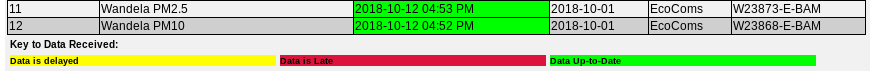
\includegraphics[width=\textwidth]{images/ecstat_status.png}
    \caption[Ecostat.co.za status report]{Caption}
    \label{fig:ecostat_status}
\end{figure}

Ecostat further allows quick view products of the instrument status,
meteorological and pollution data from the site location as seen
in \hyperref[fig:ecostat_quick]{figure \ref{fig:ecostat_quick}}. This is
valuable to quickly asses current ambient environment and also to check the
instrument for unrealistic or erroneous values.

\begin{figure}[!htb]
    \centering
    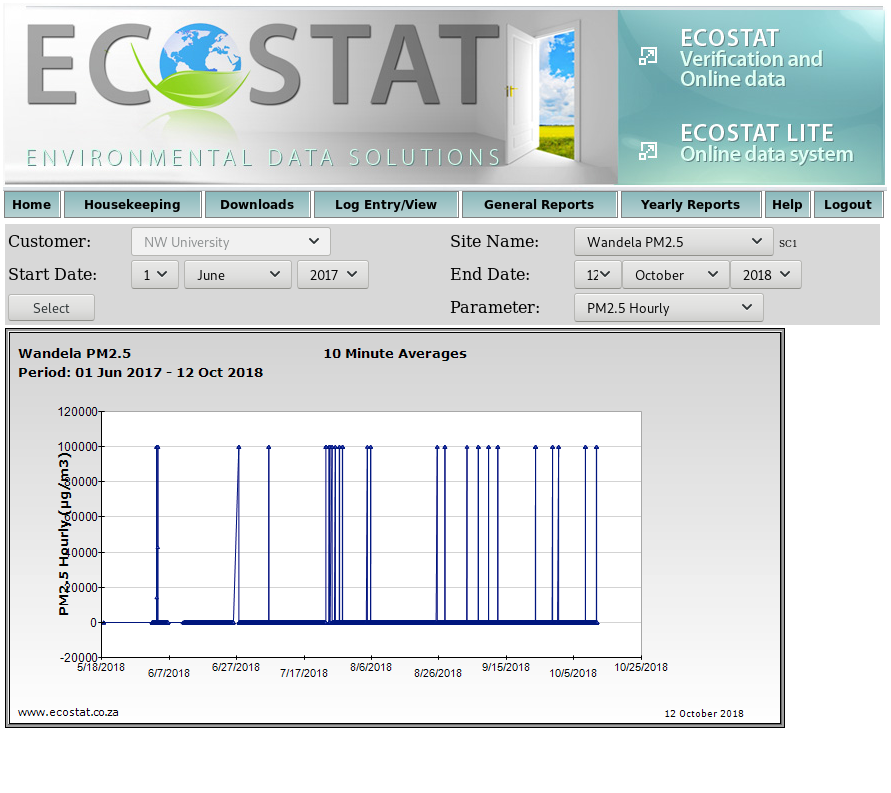
\includegraphics[width=\textwidth]{images/ecostat_quick.png}
    \caption[Ecostat.co.za quick view]{Caption}
    \label{fig:ecostat_quick}
\end{figure}

%%%%%%%%%%%%%%%%%%%%%%%%%%%%%%%%%%%%%%%%%%%%%%%%%%%%%%%%%%%%%

\chapter{Site preparation and installation}

\section{Identifying potential sites}

\section{Electricity supply for the instrument}

\section{Security and access control}
All instruments are located within a fenced perimeter in Wadela. Only technicians and
research staff have access to the site.

\begin{figure}[!htb]
    \centering
    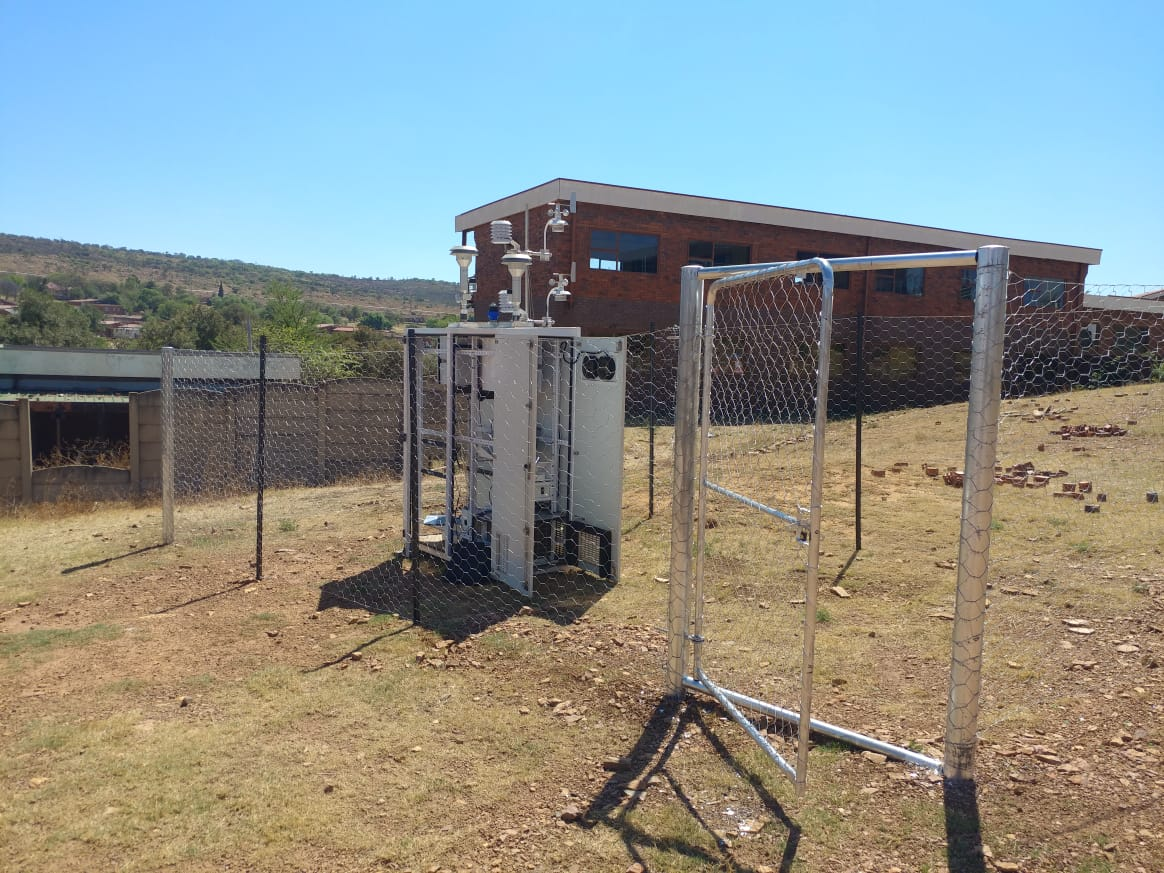
\includegraphics[width=\textwidth]{images/wedela_4.jpeg}
    \caption[Security and access control at the Wedela measuring site]{Security and access control at the Wedela measuring site}
    \label{fig:wadela_fence}
\end{figure}

\section{Community engagement}

%%%%%%%%%%%%%%%%%%%%%%%%%%%%%%%%%%%%%%%%%%%%%%%%%%%%%%%%%%%%%

\chapter{Measurements of atmospheric particulate matter}

\section{File conventions}

All final datasets are stored in \gls{ascii} format with extensions
``.txt'' and ``.csv''. This is the most
widely accepted format readable by most software. The most common
convention is simple \gls{csv}, usually denoted with the extension
``.csv''. Most of the data acquisition devices
store data in \gls{ascii}, these raw files are kept untouched. All
binary formats are converted into \gls{csv} files. Staring all
data-sets in \gls{ascii} will ensure that all users will have easy
access to the data and any future changes to commercial software will
not impact on its accessibility.

Excel is the most common software used for data processing. \gls{csv}
files easily integrates with most import and export facilities of
Excel. Special care must be taken when using the following features:

\begin{description}
\item [Importing files] A field separator should be chosen when
  importing files into Excel. The default separator is a comma
  (,). This implies that a comma should not be used anywhere in data
  files other than for denoting a field separator. It is very likely
  that commas will be present if there are long strings or written
  descriptions in a file. In these cases, a pipe (\textbar) can be used as a
  separator. These instances should be avoided as far as possible.
\item [Formatting of cells] Care must be exercised when processing or
  formatting data in excel. The formatting of each cell in Excel
  depends on the settings. It frequently looks different from the raw
  data. If the user are not aware of the current formatting setting of
  the cell, row or column, mistakes will be made when importing or
  exporting data. The most common places for these mistakes comes when
  dealing with dates, times, percentages and decimal characters.
\item [Exporting files] Final data-sets is stored in \gls{csv}. This is
  a standard export feature of Excel. The following features of most
  current versions of Excel must be taken into consideration when
  exporting files to \gls{csv}. If the Excel files contains many
  sheets, only the active sheet will be saved to \gls{csv} per export
  action. Each sheet must therefore be saved to a separate file.
\item [Using inverted commas (``)] Inverted commas typically has a
  special meaning in Excel. It is used to denote a text string for
  that particular field. When encapsulating data points in inverted
  commas, the user invariable forces Excel to see that field as a text
  string. This will be problematic if the user wishes to use that
  field in any operations, like algebraic conversion or time series
  operations. For this reason, inverted commas should only be used to
  denote text strings. An example would be to prevent excel from splitting a
  long text description containing commas into fields when importing a
  \gls{csv} files with a comma as a separator.
\end{description}

\subsubsection{General procedure for data quality control}
The raw data-sets collected are merged and processed into a final data
set for analysis through the following steps:

\begin{enumerate}
\item Apply date and time corrections to each of the raw data files
  using the instrument logs
\item Merge each of the data-sets above into one uniform data-set
\item Apply masks to each instrument according to the instrument log
\item Perform automated quality control on each variable and flag problematic values
  \begin{itemize}
   \item Test for sensible observation date and time values.
   \item Flag data close to or below the instrument detection limit. 
   \item Flag data close to or above the instrument's maximum detectable limited
   \item Test the gradient of each instrument against realistic response times
   \item Test for spikes by comparing with values before and after
   \item Test for stuck values and set missing
   \item Flag climatological outliers
   \item Flag outliers using the median absolute deviation
  \end{itemize}
\item Each variable with its associated flags identified in the automated quality control is then reviewed manually by viewing time series plots. Each flag is carefully inspected and values are deemed real or set to missing if a problem is suspected.
\item Values close to or below the detection limit are finally set to the minimum detection limit of the particular instrument \citep{Croghan2003}.
\end{enumerate}

The general philosophy in quality assuring data is to aggressively
ignore data that are suspected to be from a faulty instrument. Extra
care is taken when dealing with extreme values and outliers. These are
not set to missing unless they are part of a time period where the
instrument did not appear to be operating optimally.
\subsubsection{General procedure for data quality control}
The raw data-sets collected are merged and processed into a final data
set for analysis through the following steps:

\begin{enumerate}
\item Apply date and time corrections to each of the raw data files
  using the instrument logs
\item Merge each of the data-sets above into one uniform data-set
\item Apply masks to each instrument according to the instrument log
\item Perform automated quality control on each variable and flag problematic values
  \begin{itemize}
   \item Test for sensible observation date and time values.
   \item Flag data close to or below the instrument detection limit. 
   \item Flag data close to or above the instrument's maximum detectable limited
   \item Test the gradient of each instrument against realistic response times
   \item Test for spikes by comparing with values before and after
   \item Test for stuck values and set missing
   \item Flag climatological outliers
   \item Flag outliers using the median absolute deviation
  \end{itemize}
\item Each variable with its associated flags identified in the automated quality control is then reviewed manualy by viewing time series plots. Each flag is carefully inspected and values are deemed real or set to missing if a problem is suspected.
\item Values close to or below the detection limit are finally set to the minimum detection limit of the particular instrument \citep{Croghan2003}.
\end{enumerate}

The general philosophy in quality assuring data is to aggressively
ignore data that are suspected to be from a faulty instrument. Extra
care is taken when dealing with extreme values and outliers. These are
not set to missing unless they are part of a time period where the
instrument did not appear to be operating optimally.

\section{Preliminary results}

The following section shows some of the results from the Wedela monitoring site that include meteorological
and pollution data (PM2.5 and PM10). A basic QC was applied to this data-set where missing values was removed.

\begin{figure}[!htb]
    \centering
    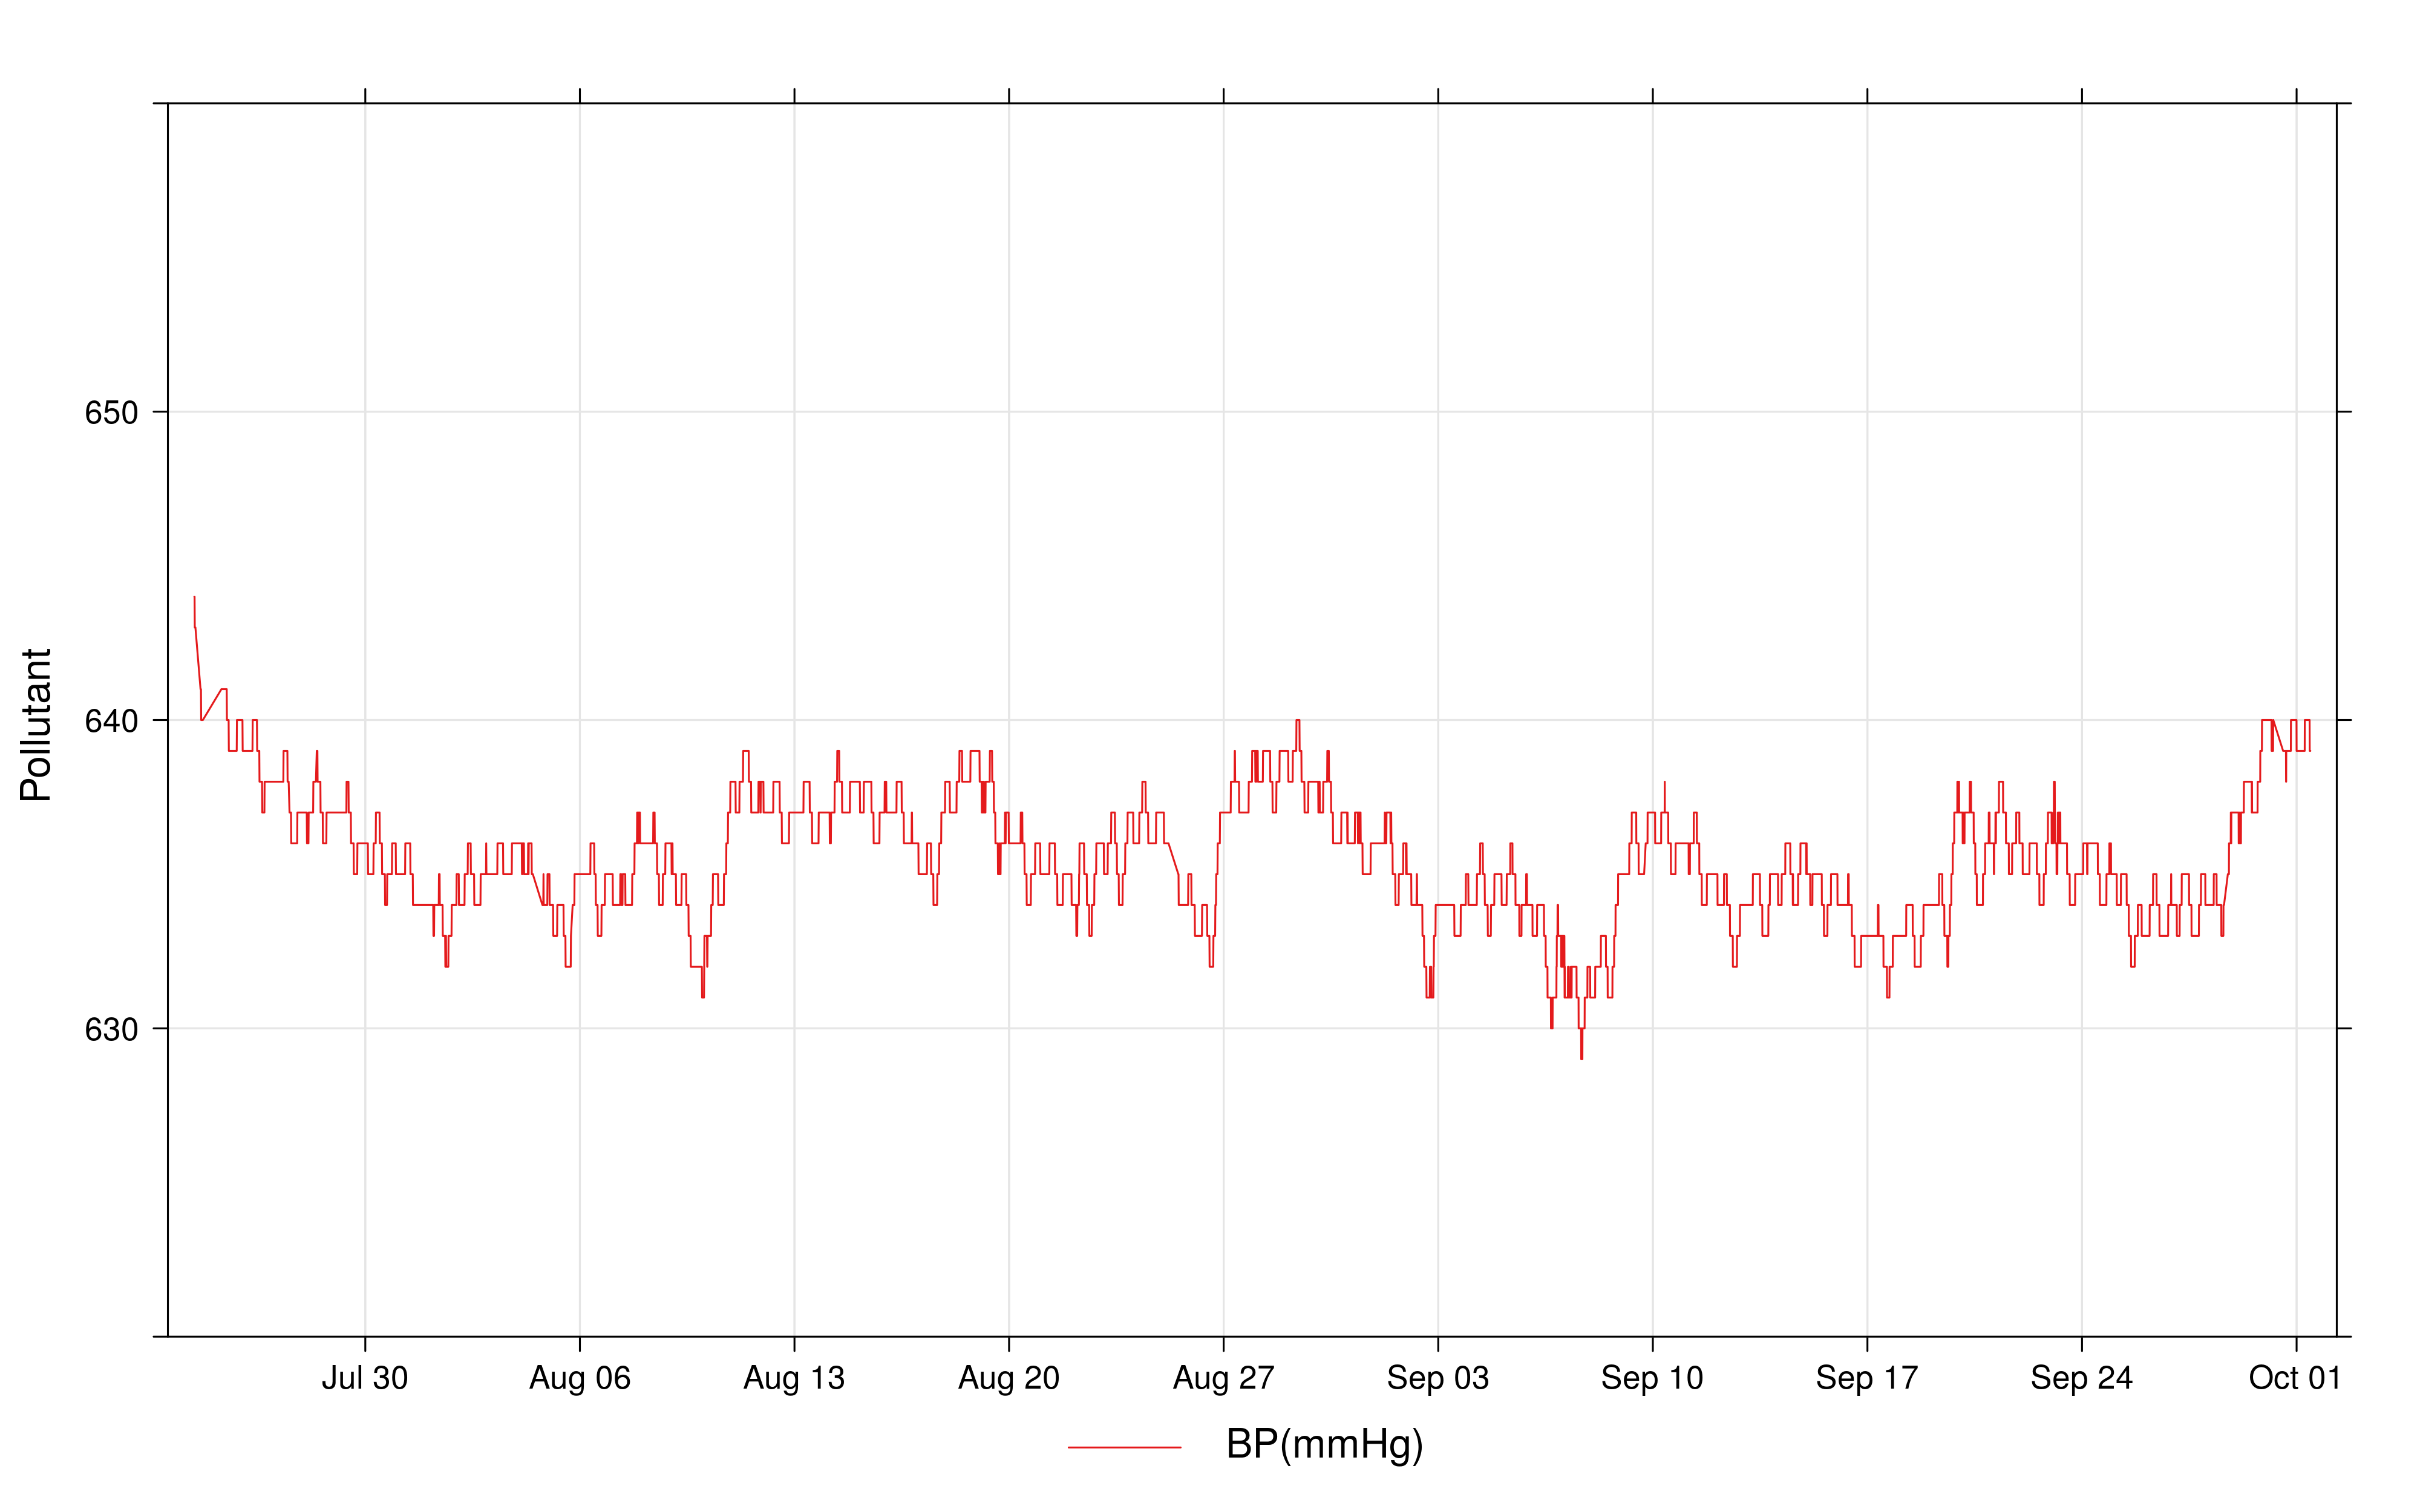
\includegraphics[width=\textwidth]{images/bp_timplt_25.png}
    \caption{Caption}
    \label{fig:pm2.5_BP_timplot}
\end{figure}

\begin{figure}[!htb]
    \centering
    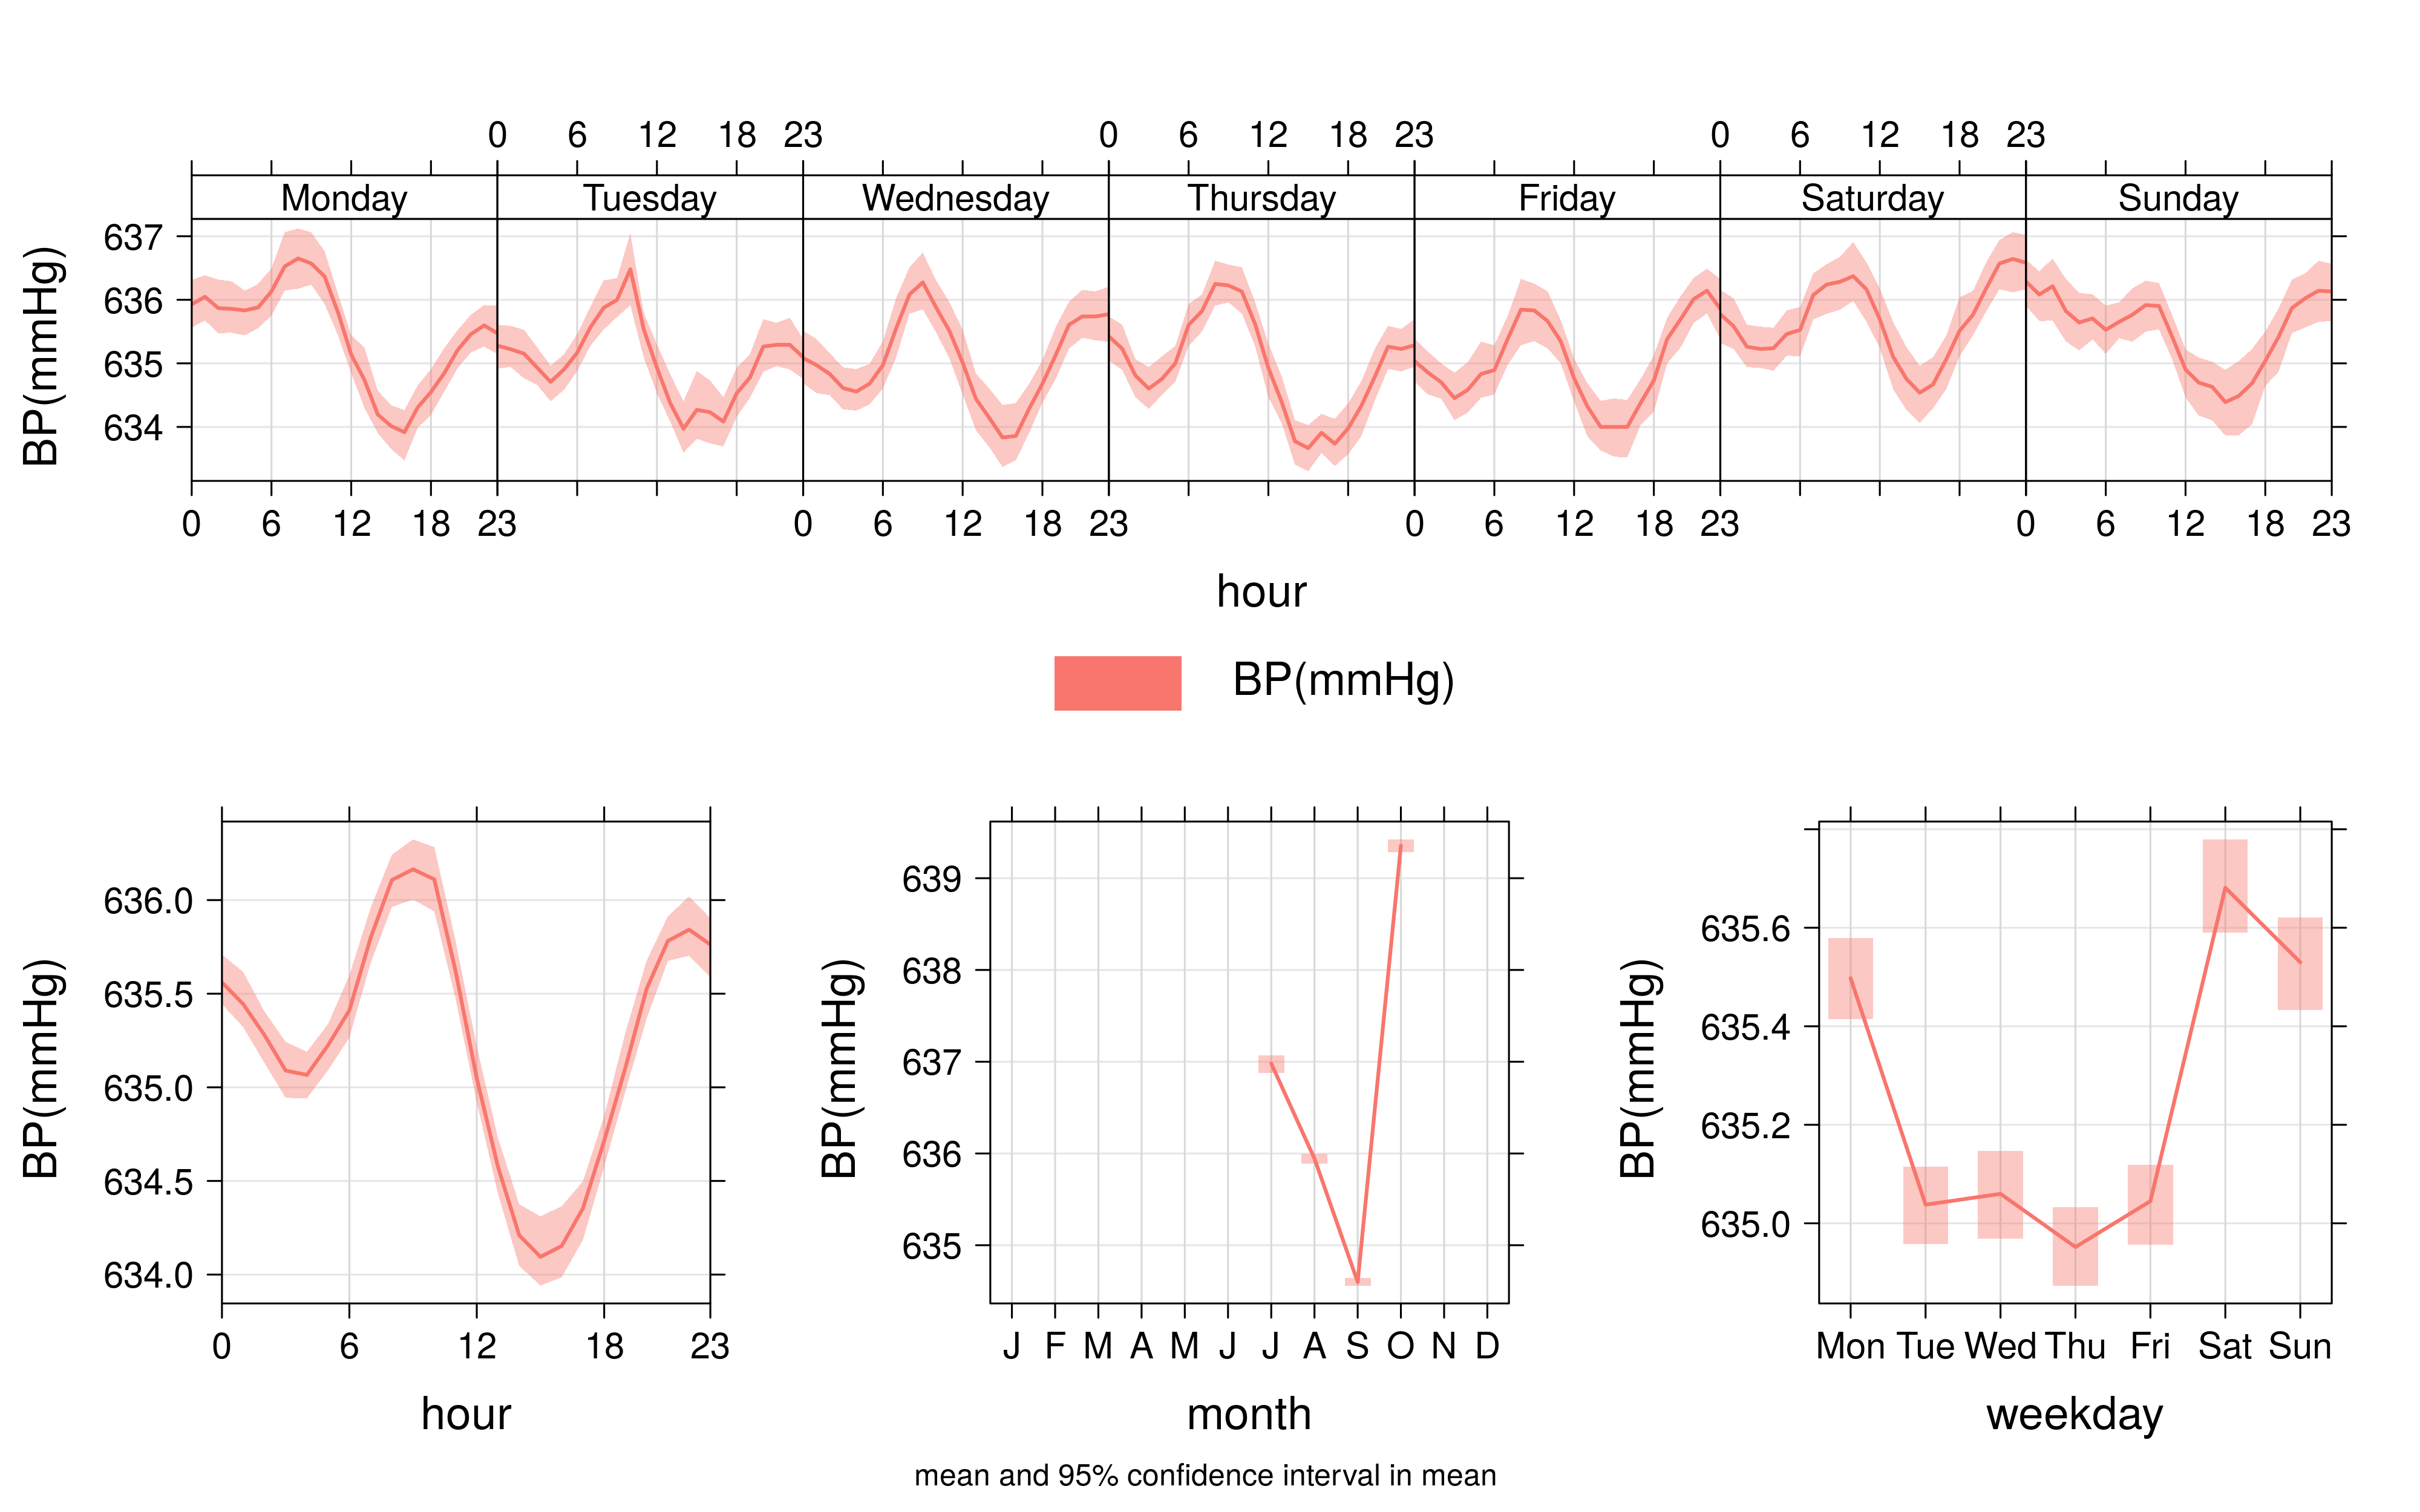
\includegraphics[width=\textwidth]{images/bp_25.png}
    \caption{Caption}
    \label{fig:pm2.5_BP}
\end{figure}

\begin{figure}[!htb]
    \centering
    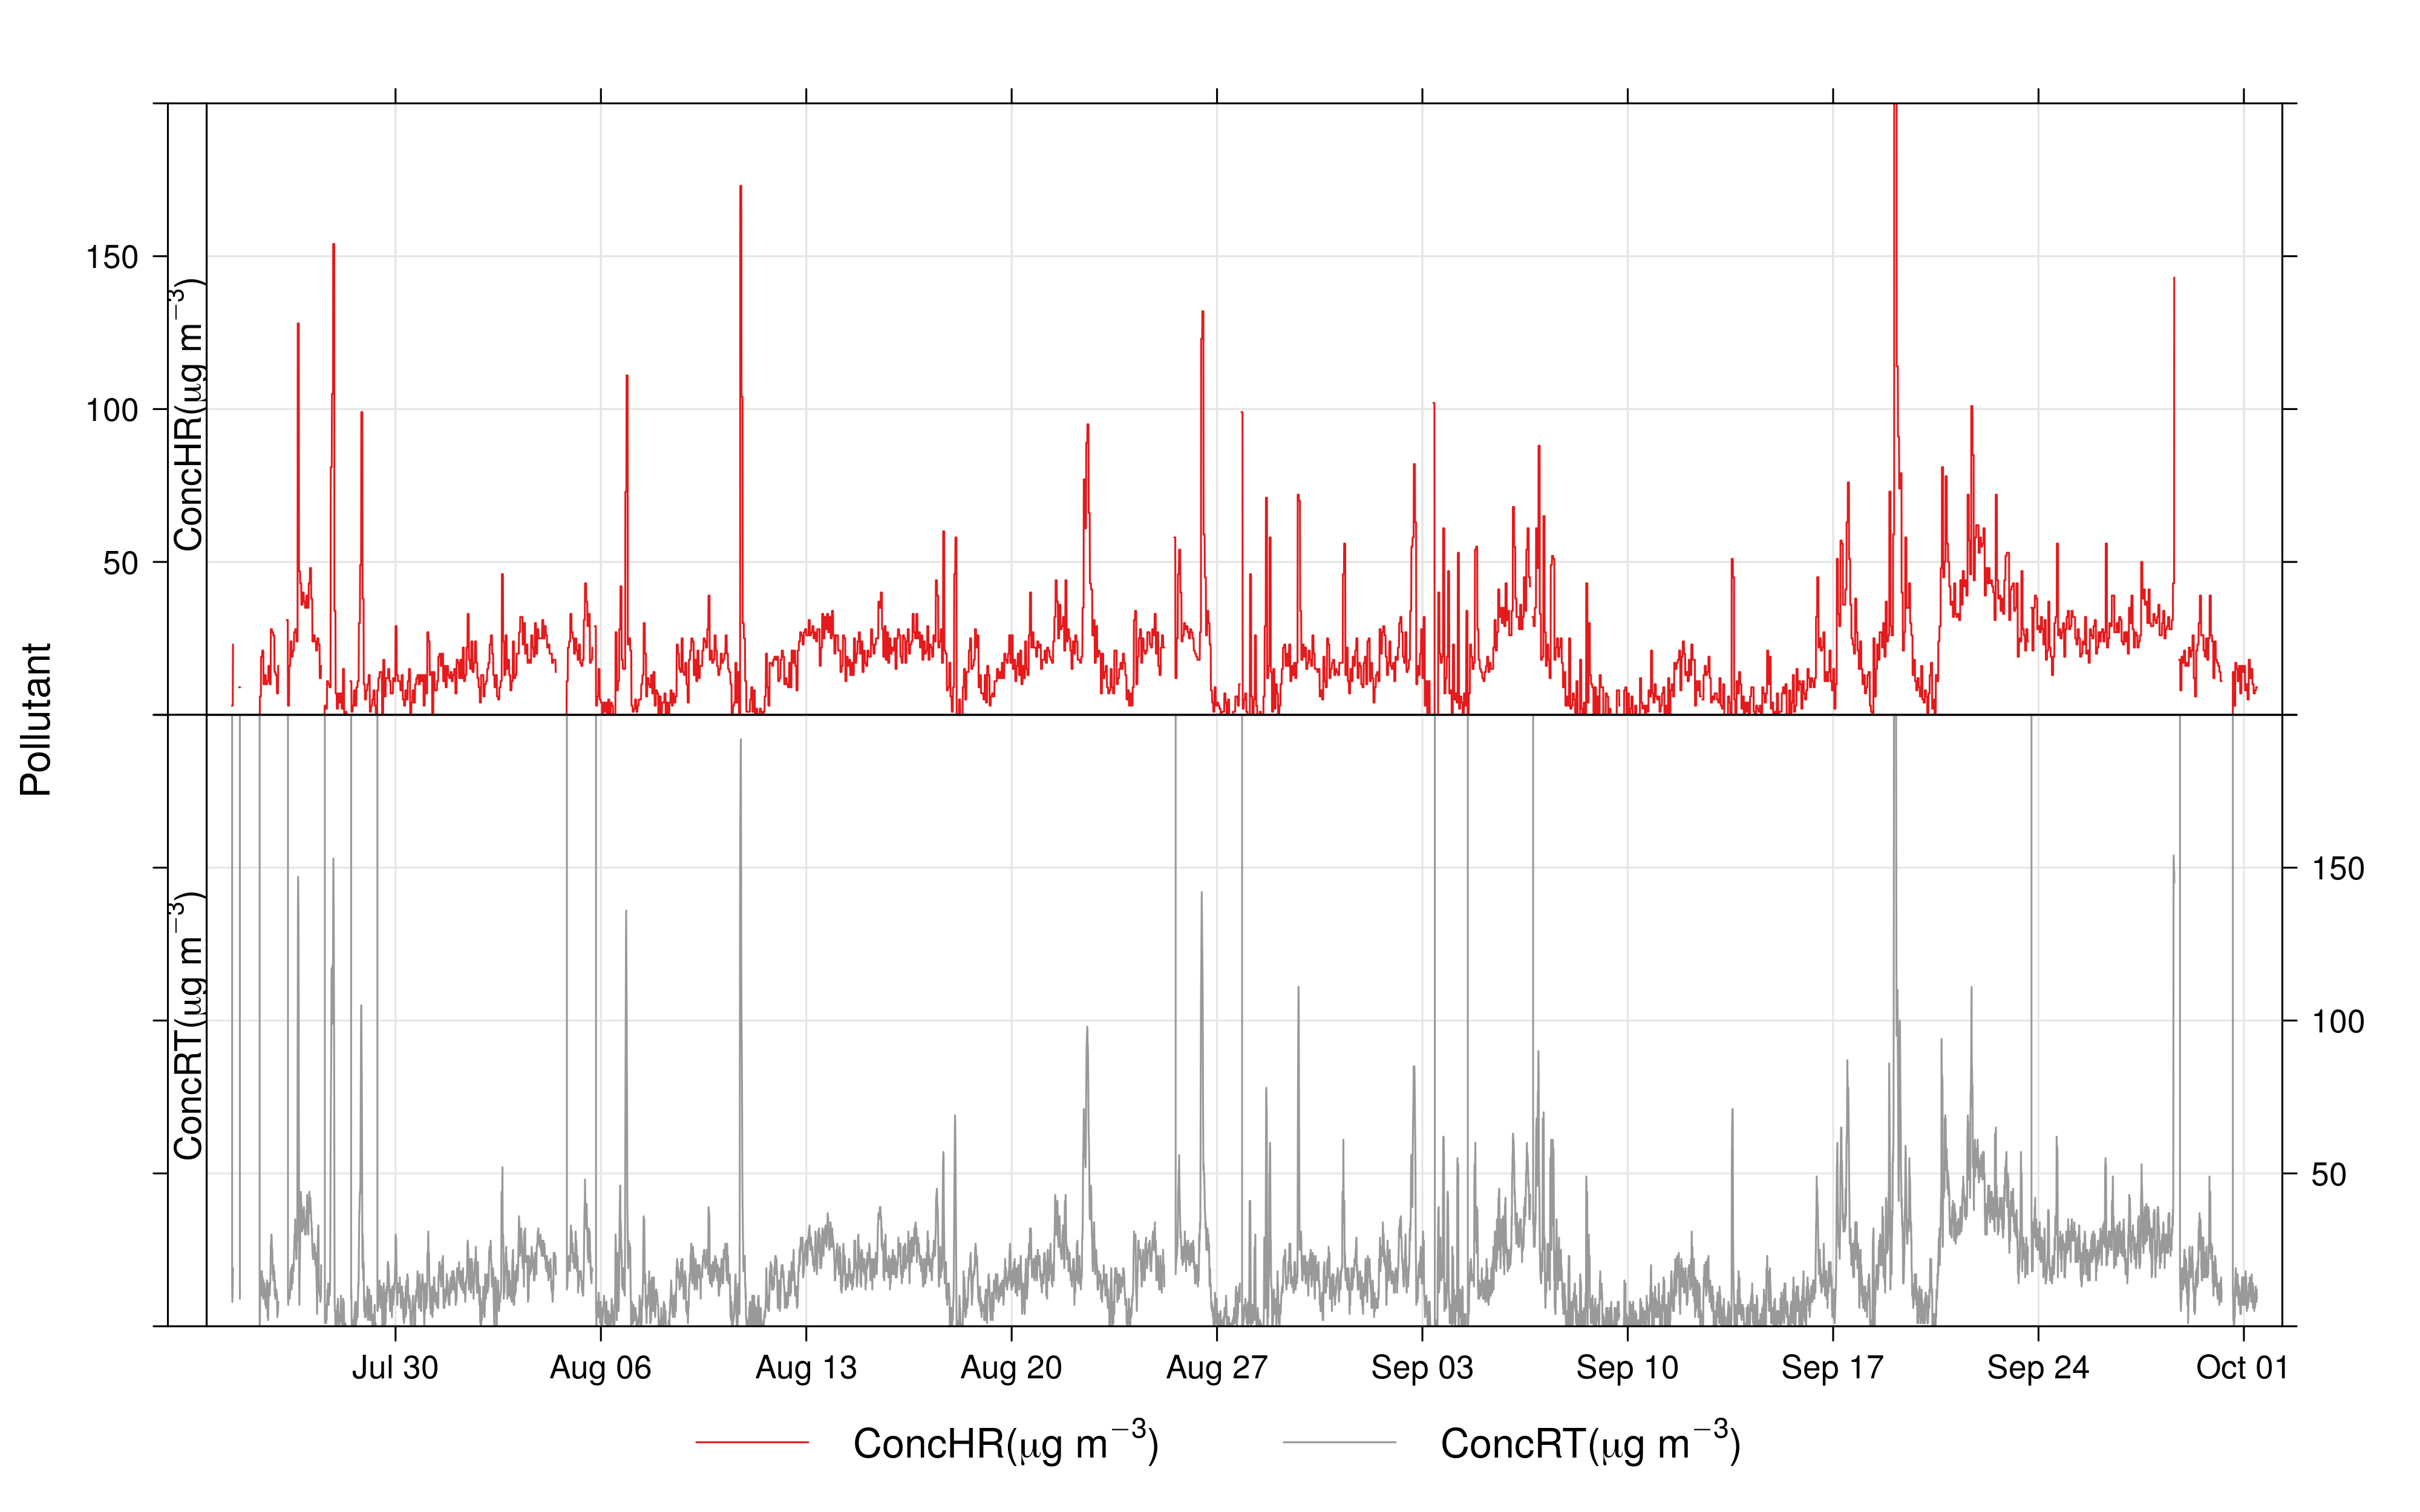
\includegraphics[width=\textwidth]{images/conc_timplt_25.png}
    \caption{Caption}
    \label{fig:pm2.5conc_timeplot}
\end{figure}

\begin{figure}[!htb]
    \centering
    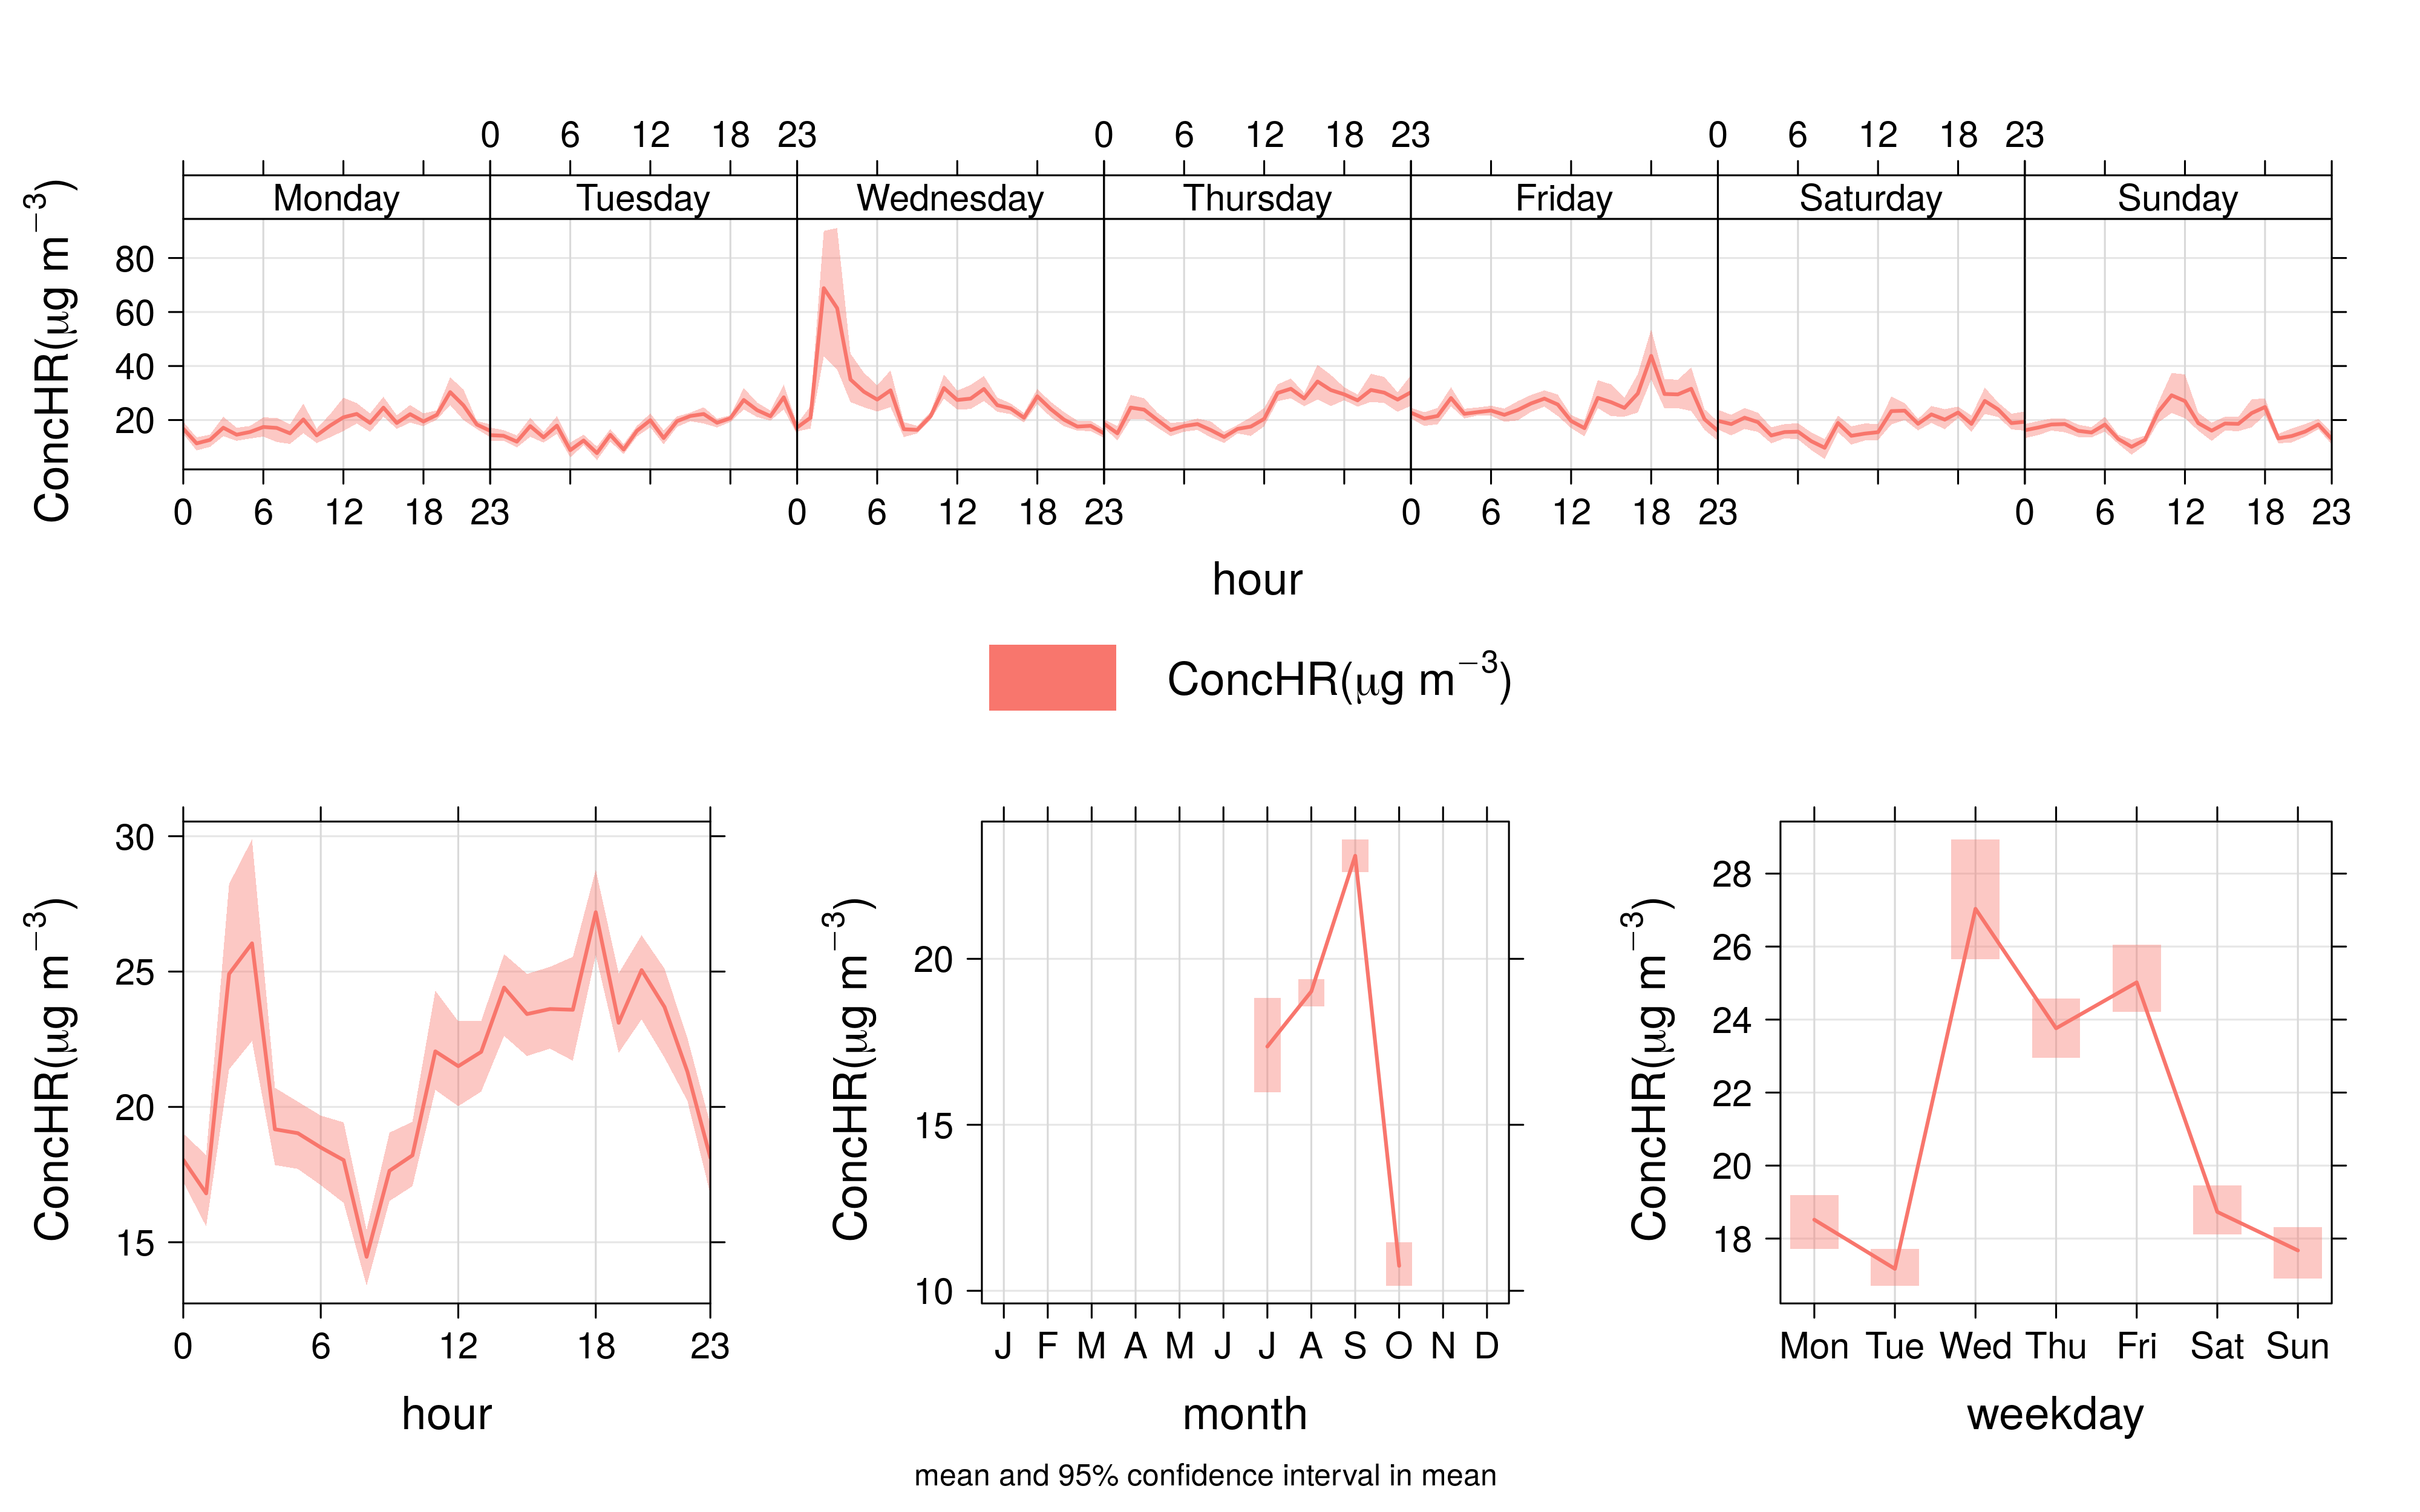
\includegraphics[width=\textwidth]{images/conc_HR_25.png}
    \caption{Caption}
    \label{fig:pm2.5conc_HR}
\end{figure}

\begin{figure}[!htb]
    \centering
    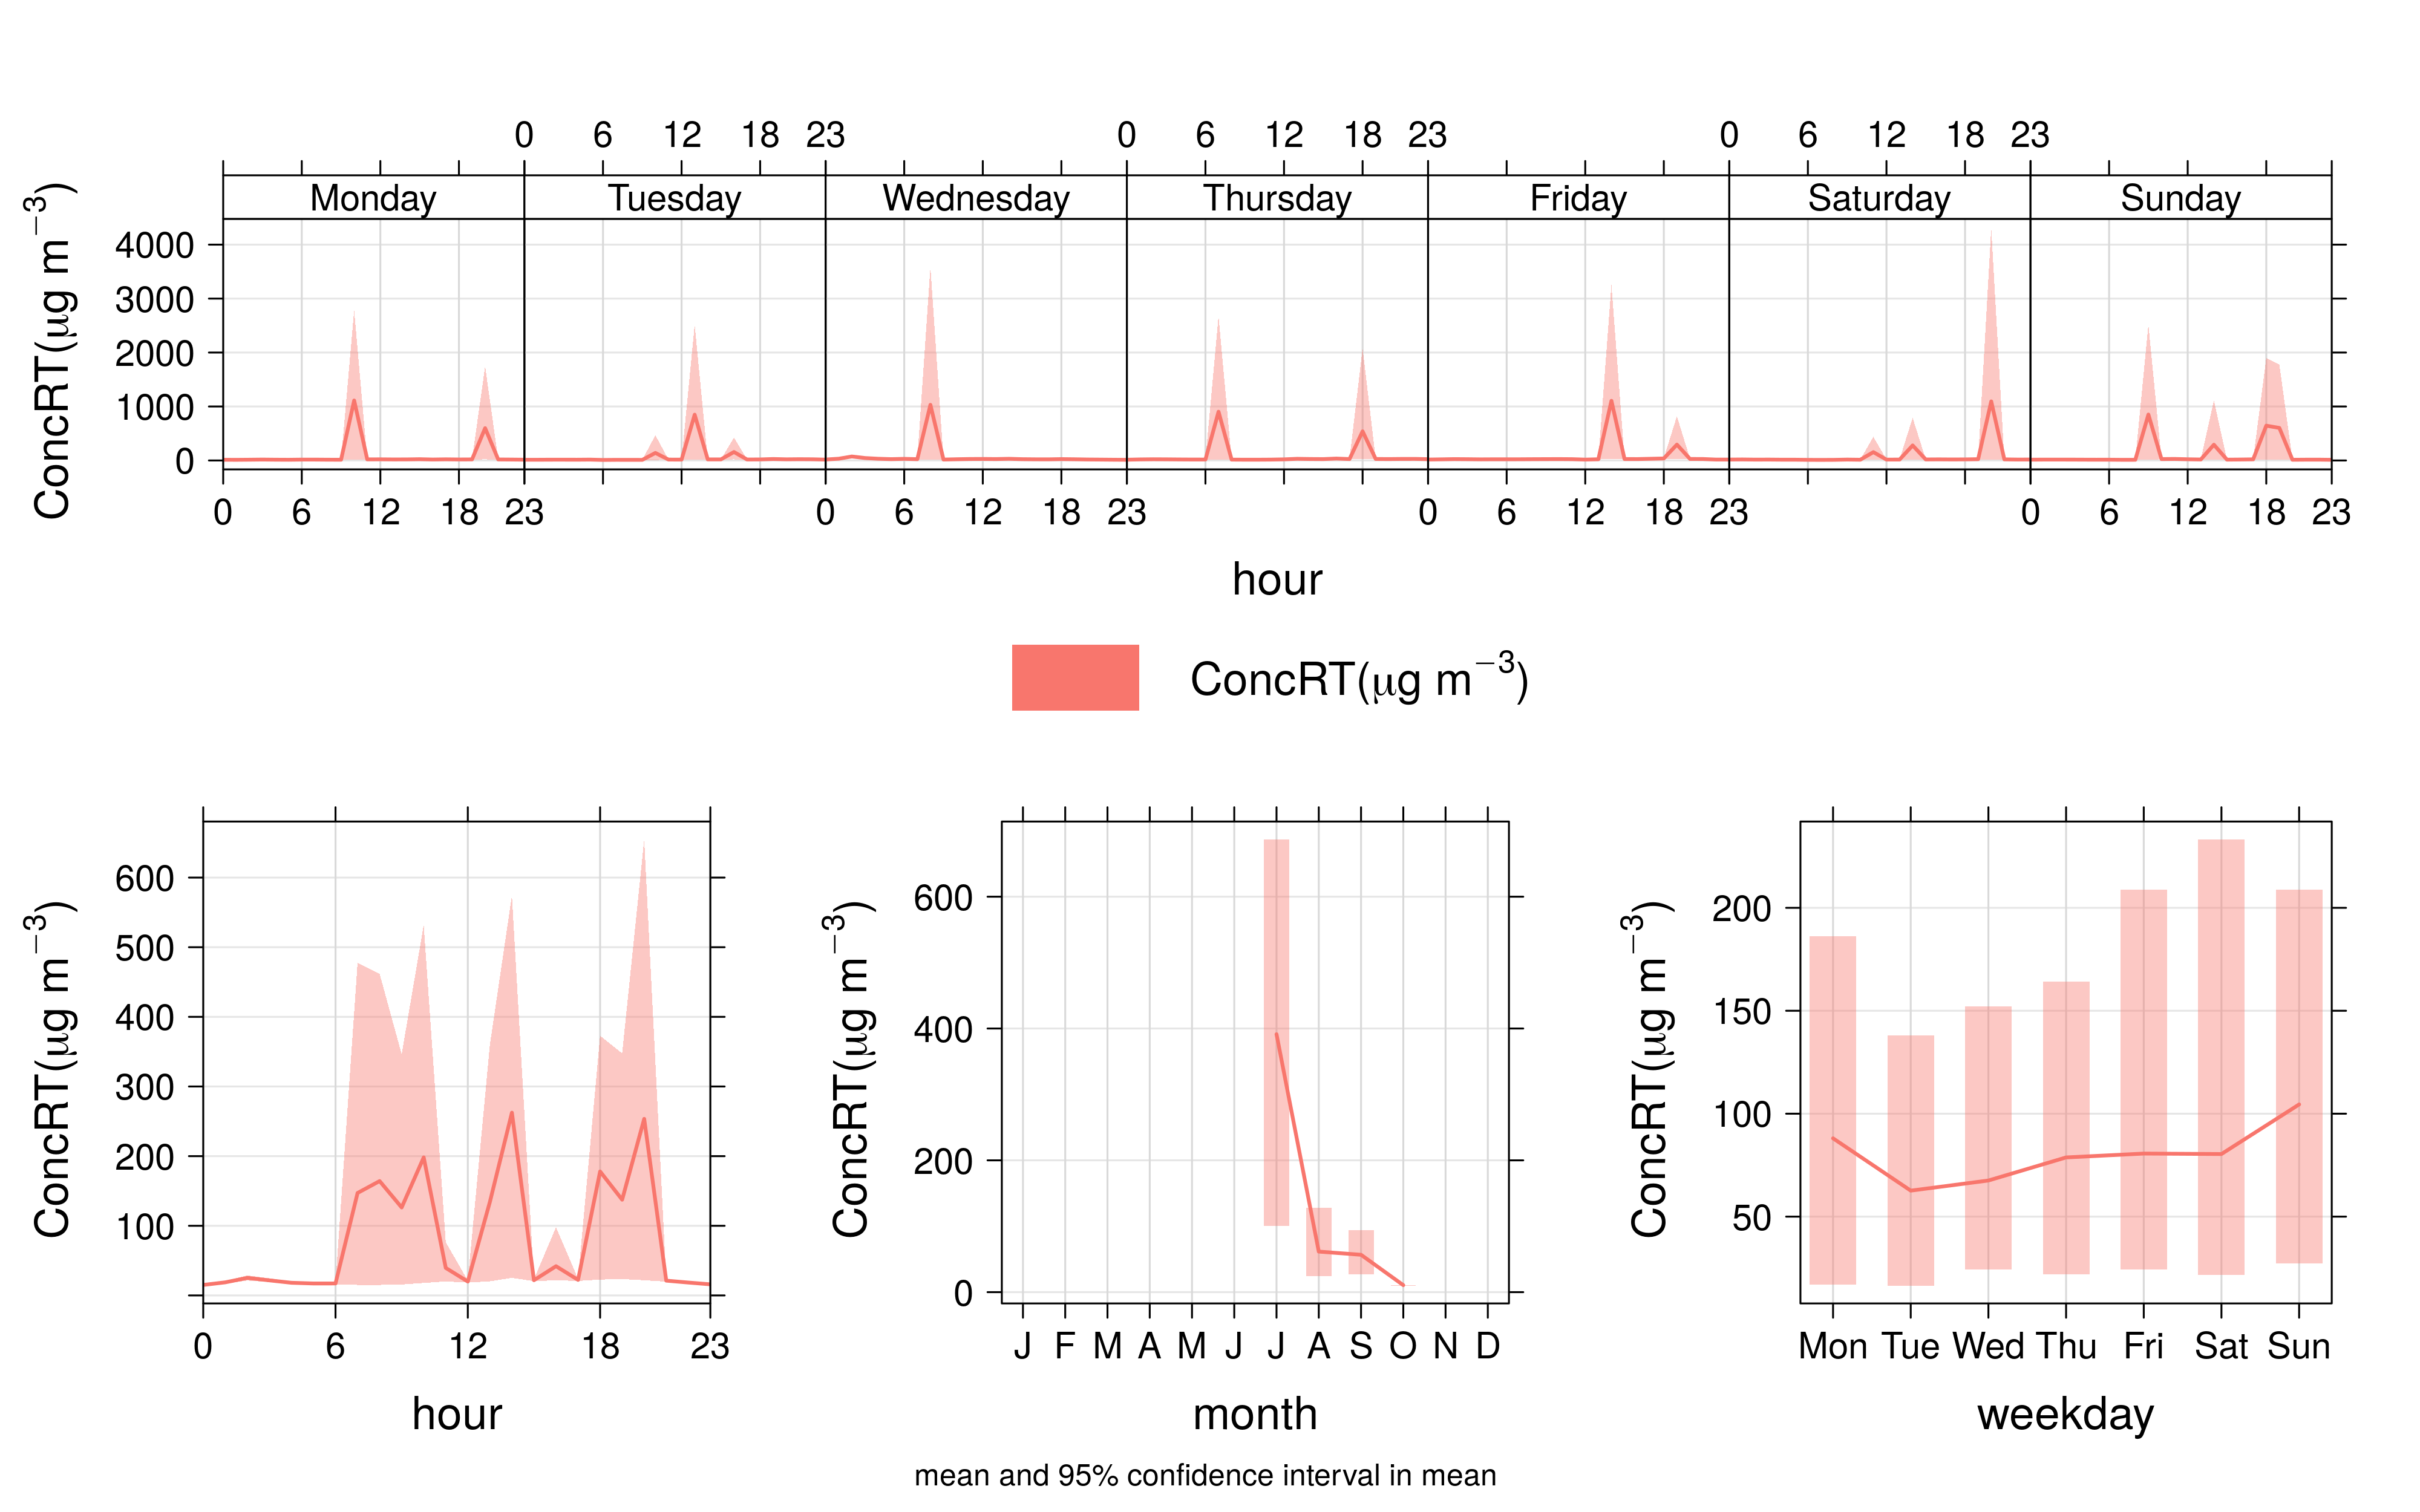
\includegraphics[width=\textwidth]{images/conc_RT_25.png}
    \caption{Caption}
    \label{fig:pm2.5conc_RT}
\end{figure}

\begin{figure}[!htb]
    \centering
    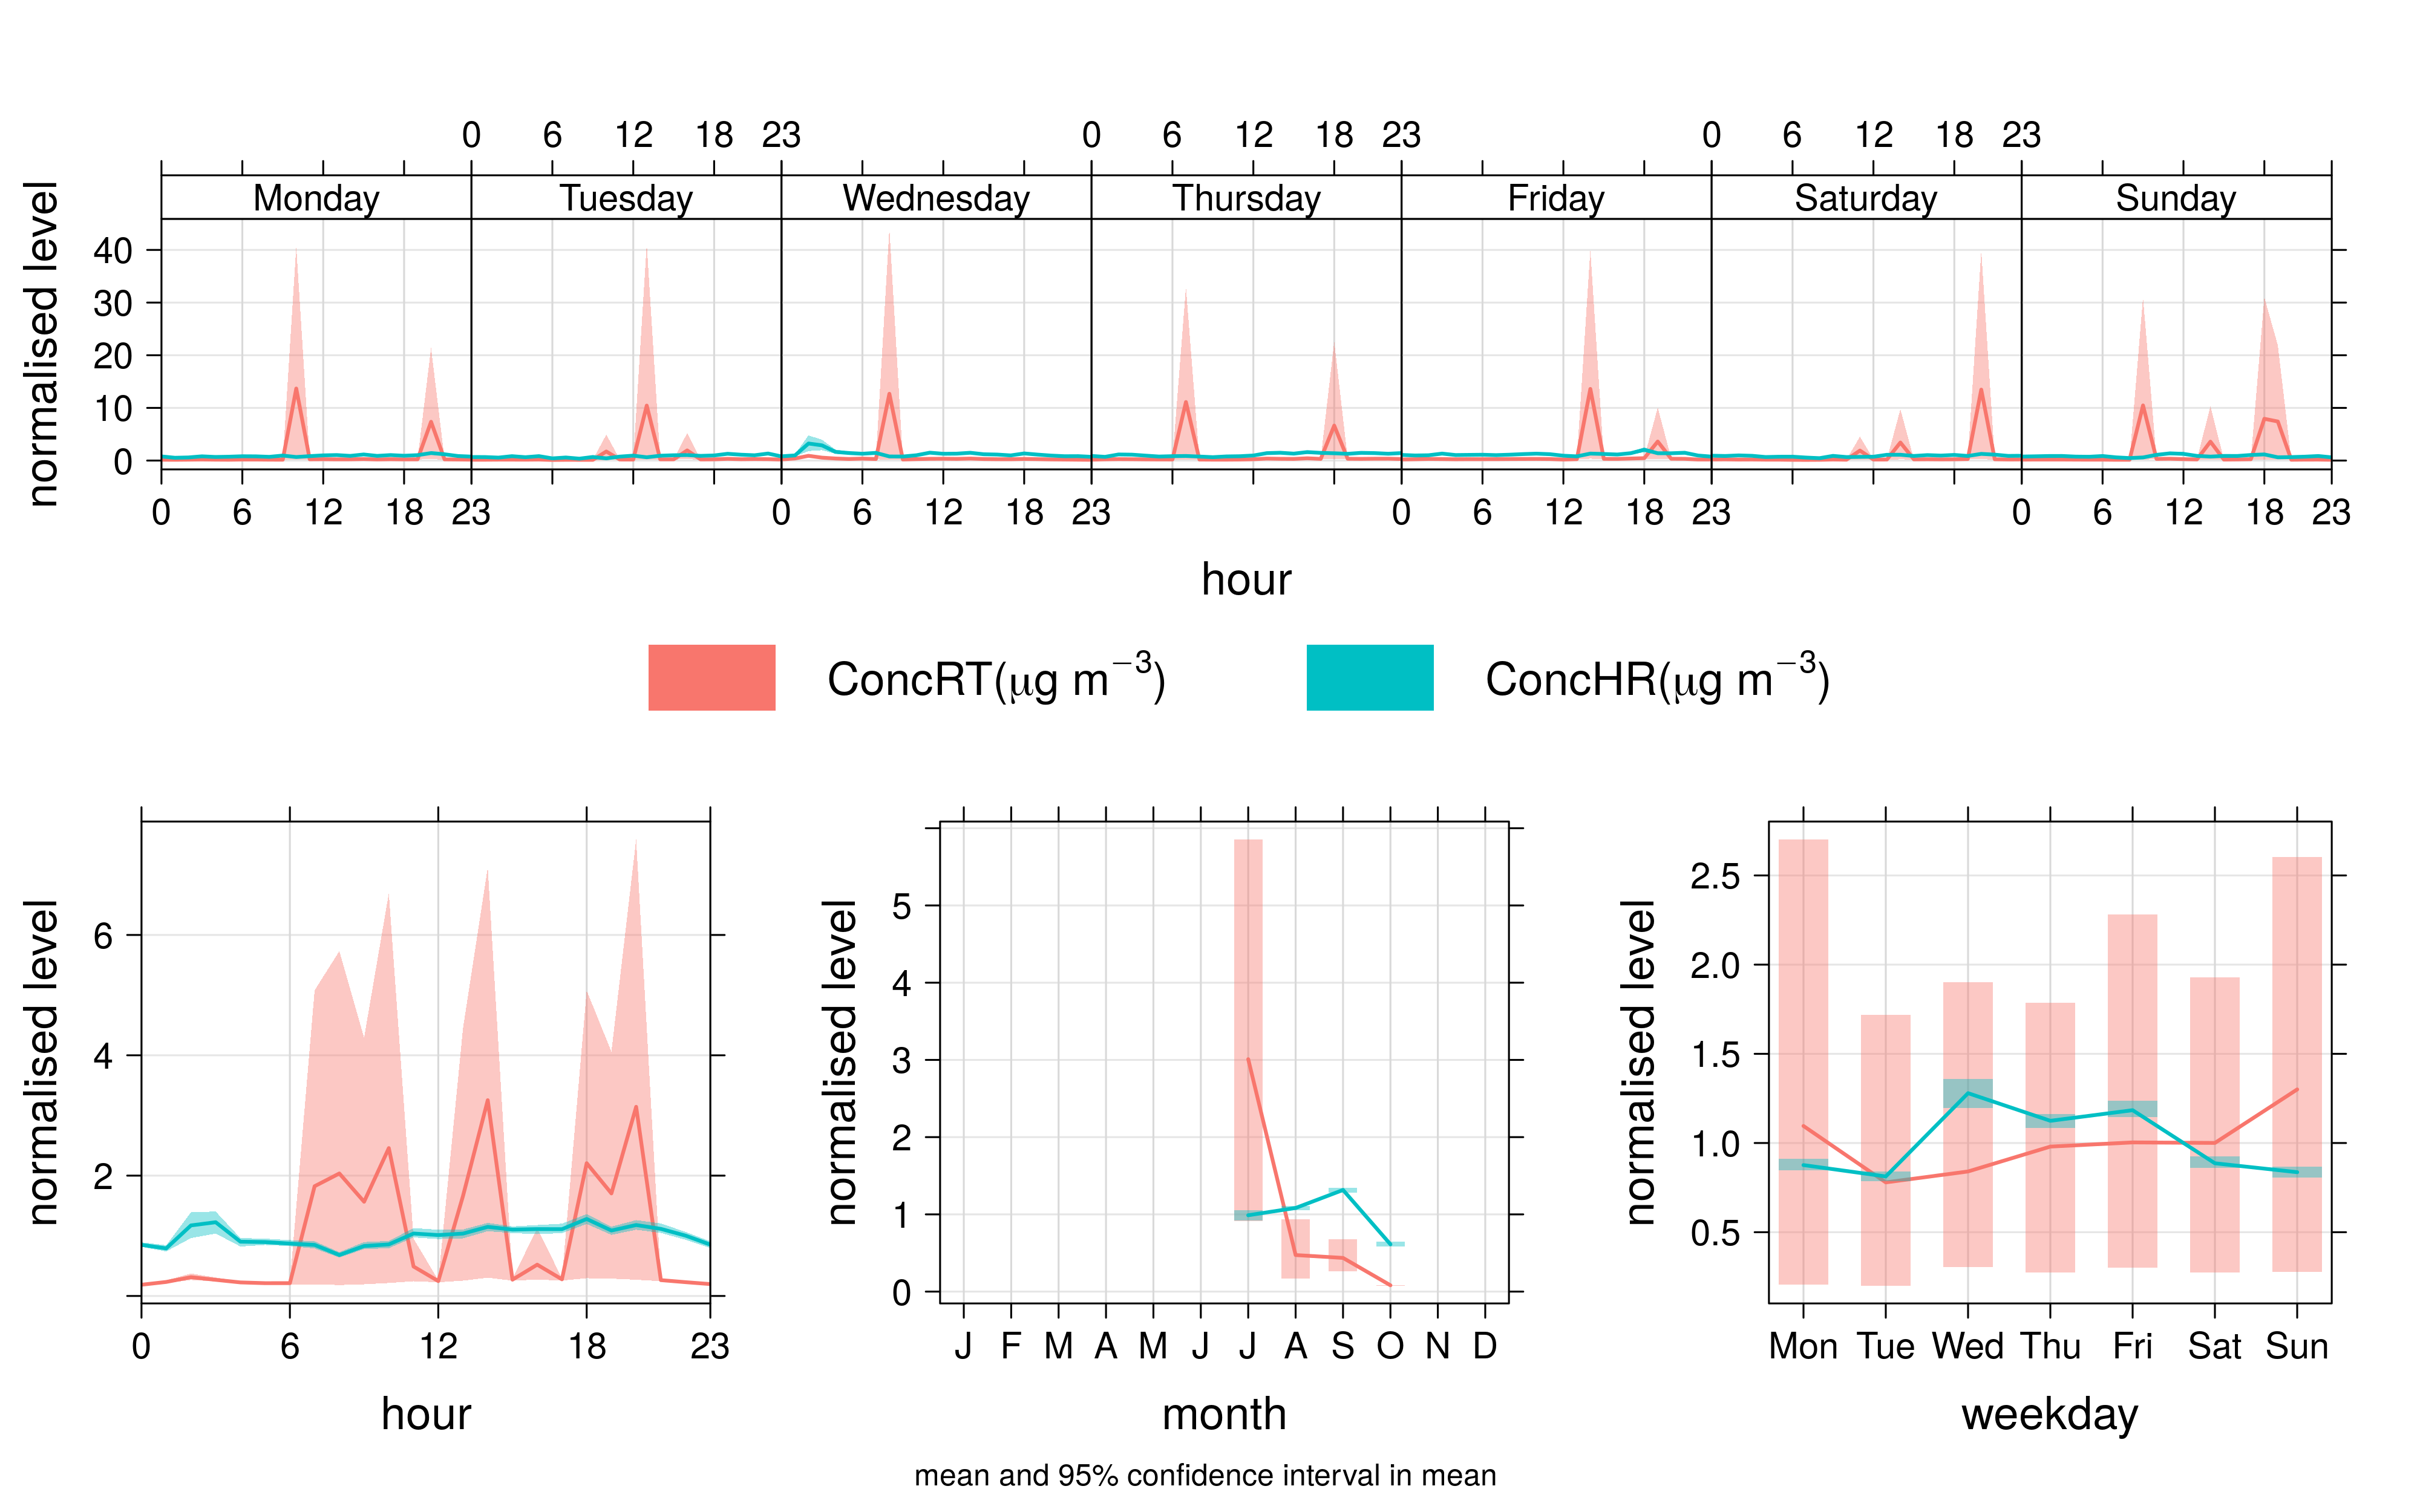
\includegraphics[width=\textwidth]{images/conc_25.png}
    \caption{Caption}
    \label{fig:pm2.5conc_all}
\end{figure}

\begin{figure}[!htb]
    \centering
    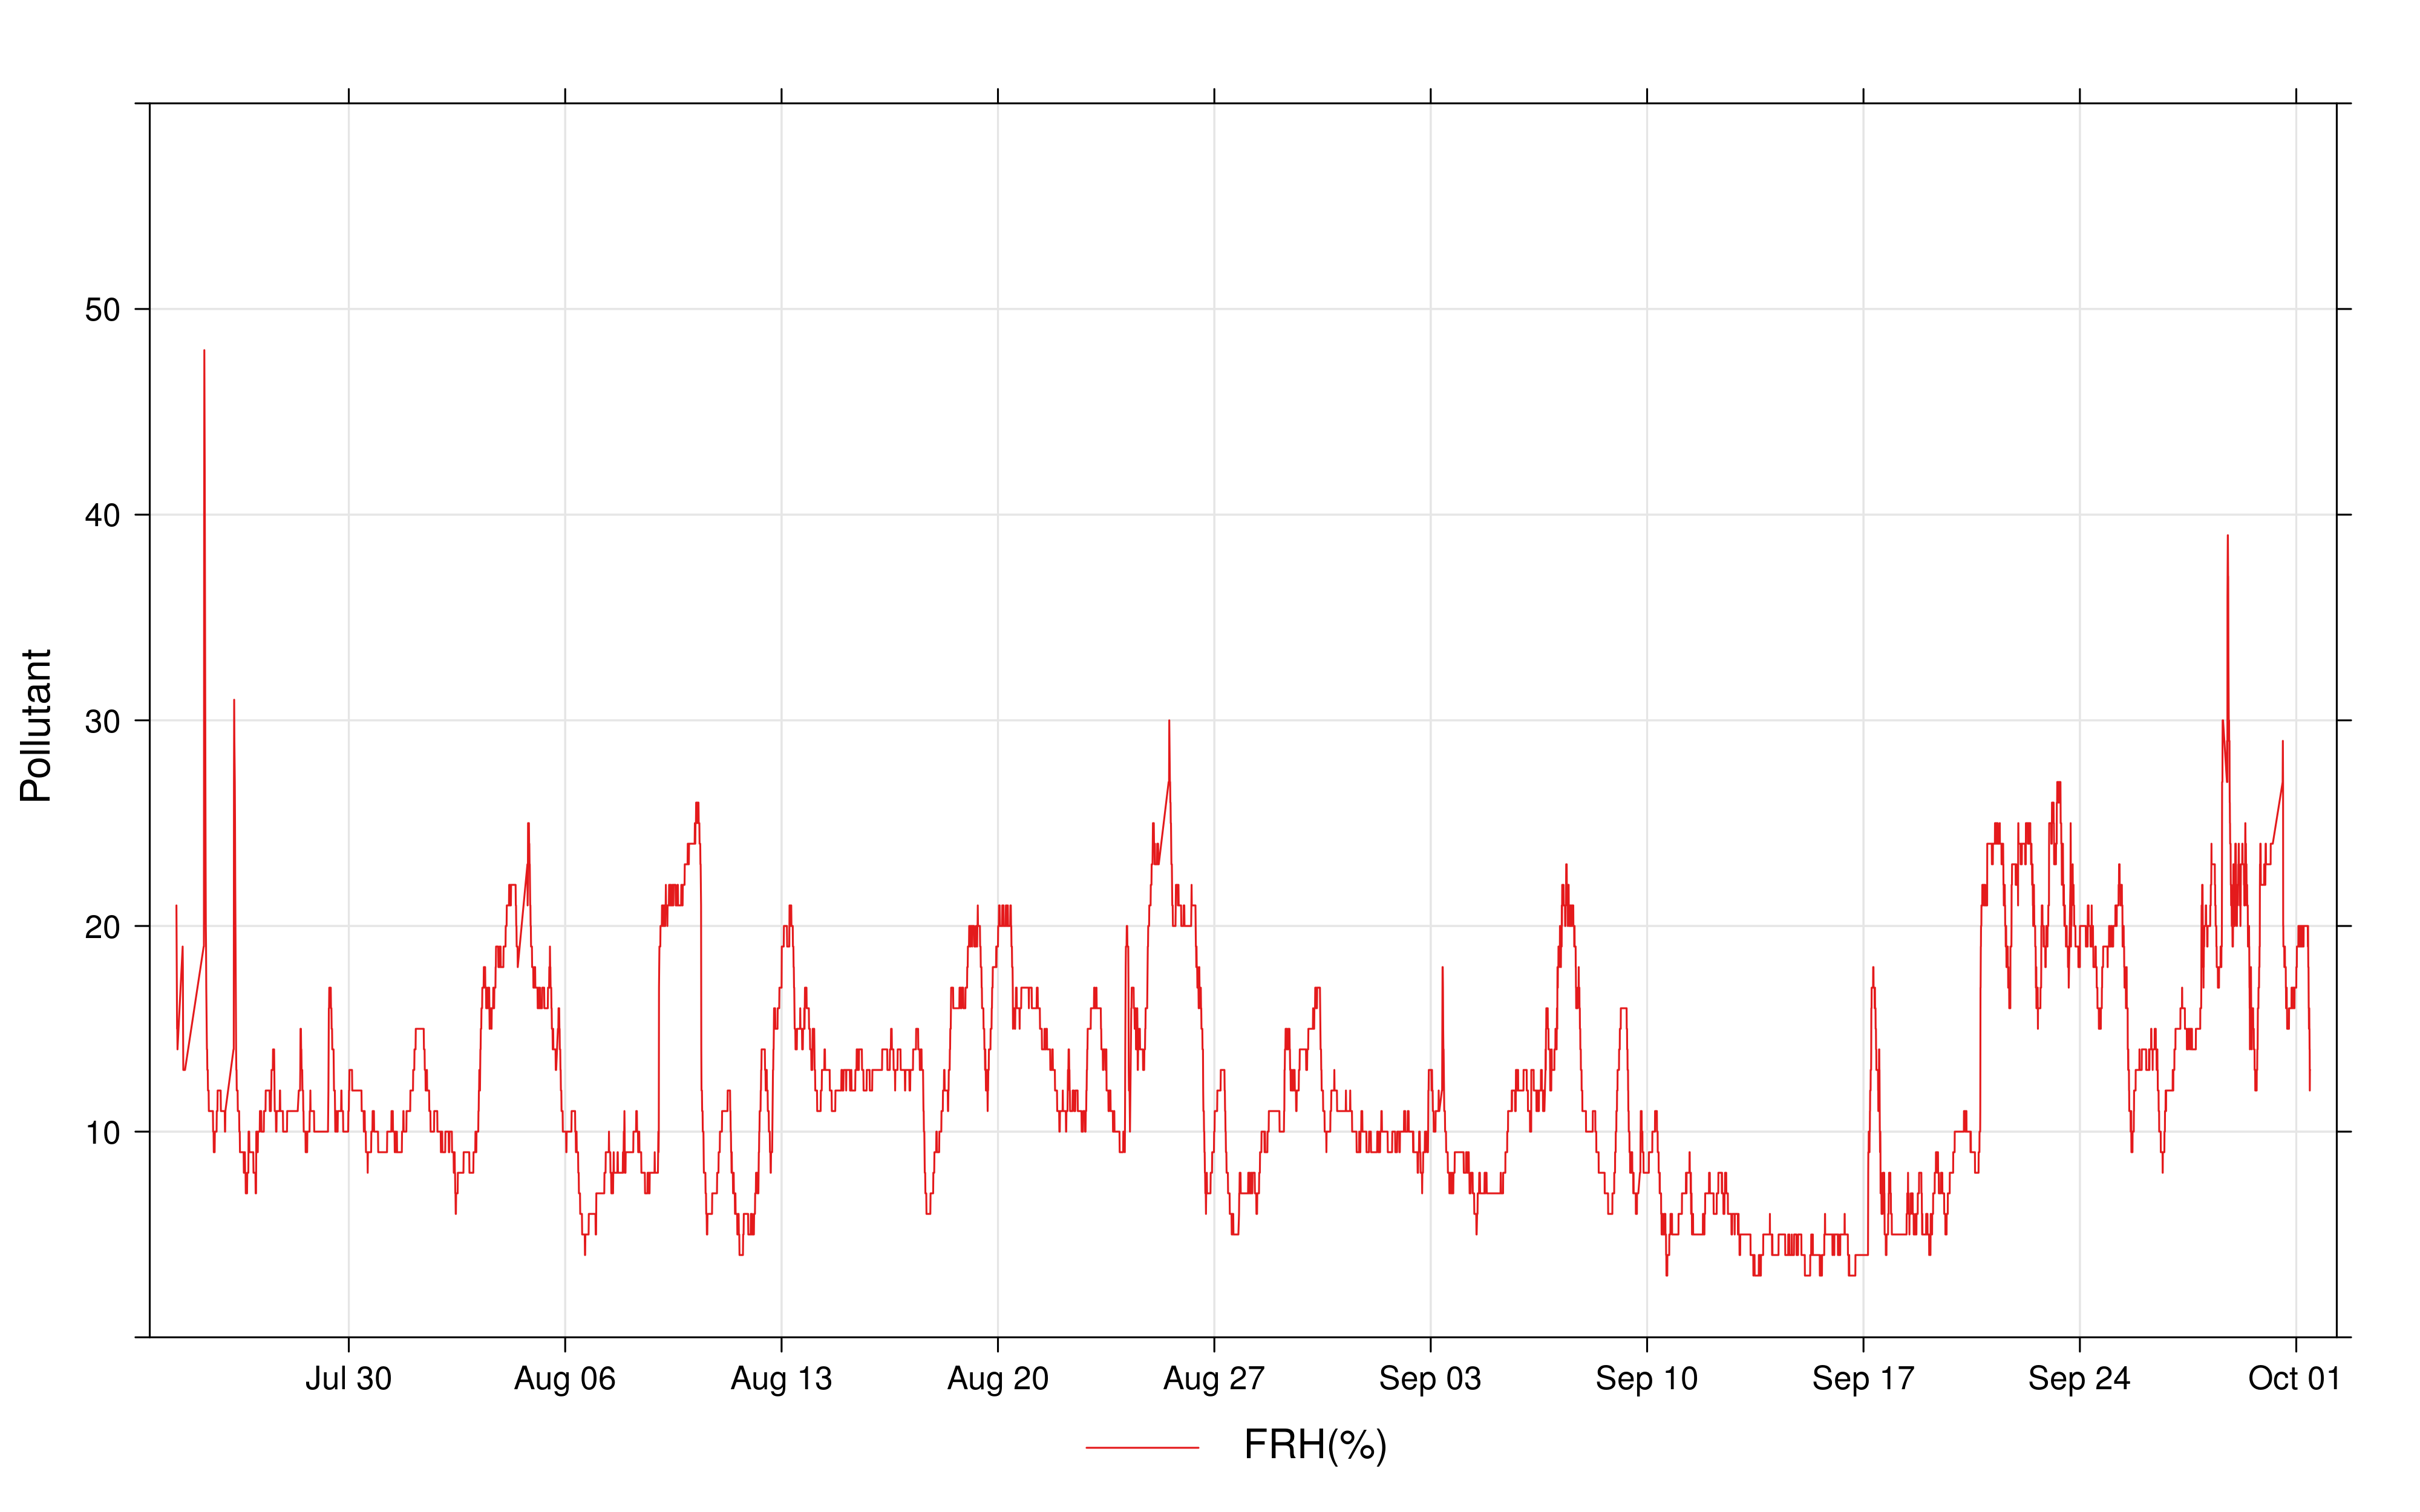
\includegraphics[width=\textwidth]{images/frh_timplt_25.png}}
    \caption{Caption}
    \label{fig:pm2.5_FR_timplot}
\end{figure}

%%%%%%%%%%%%%%%%%%%%%%%%%%%%%%%%%%%%%%%%%%%%%%%%%%%%%%%%%%%%%%%%

\begin{figure}[!htb]
    \centering
    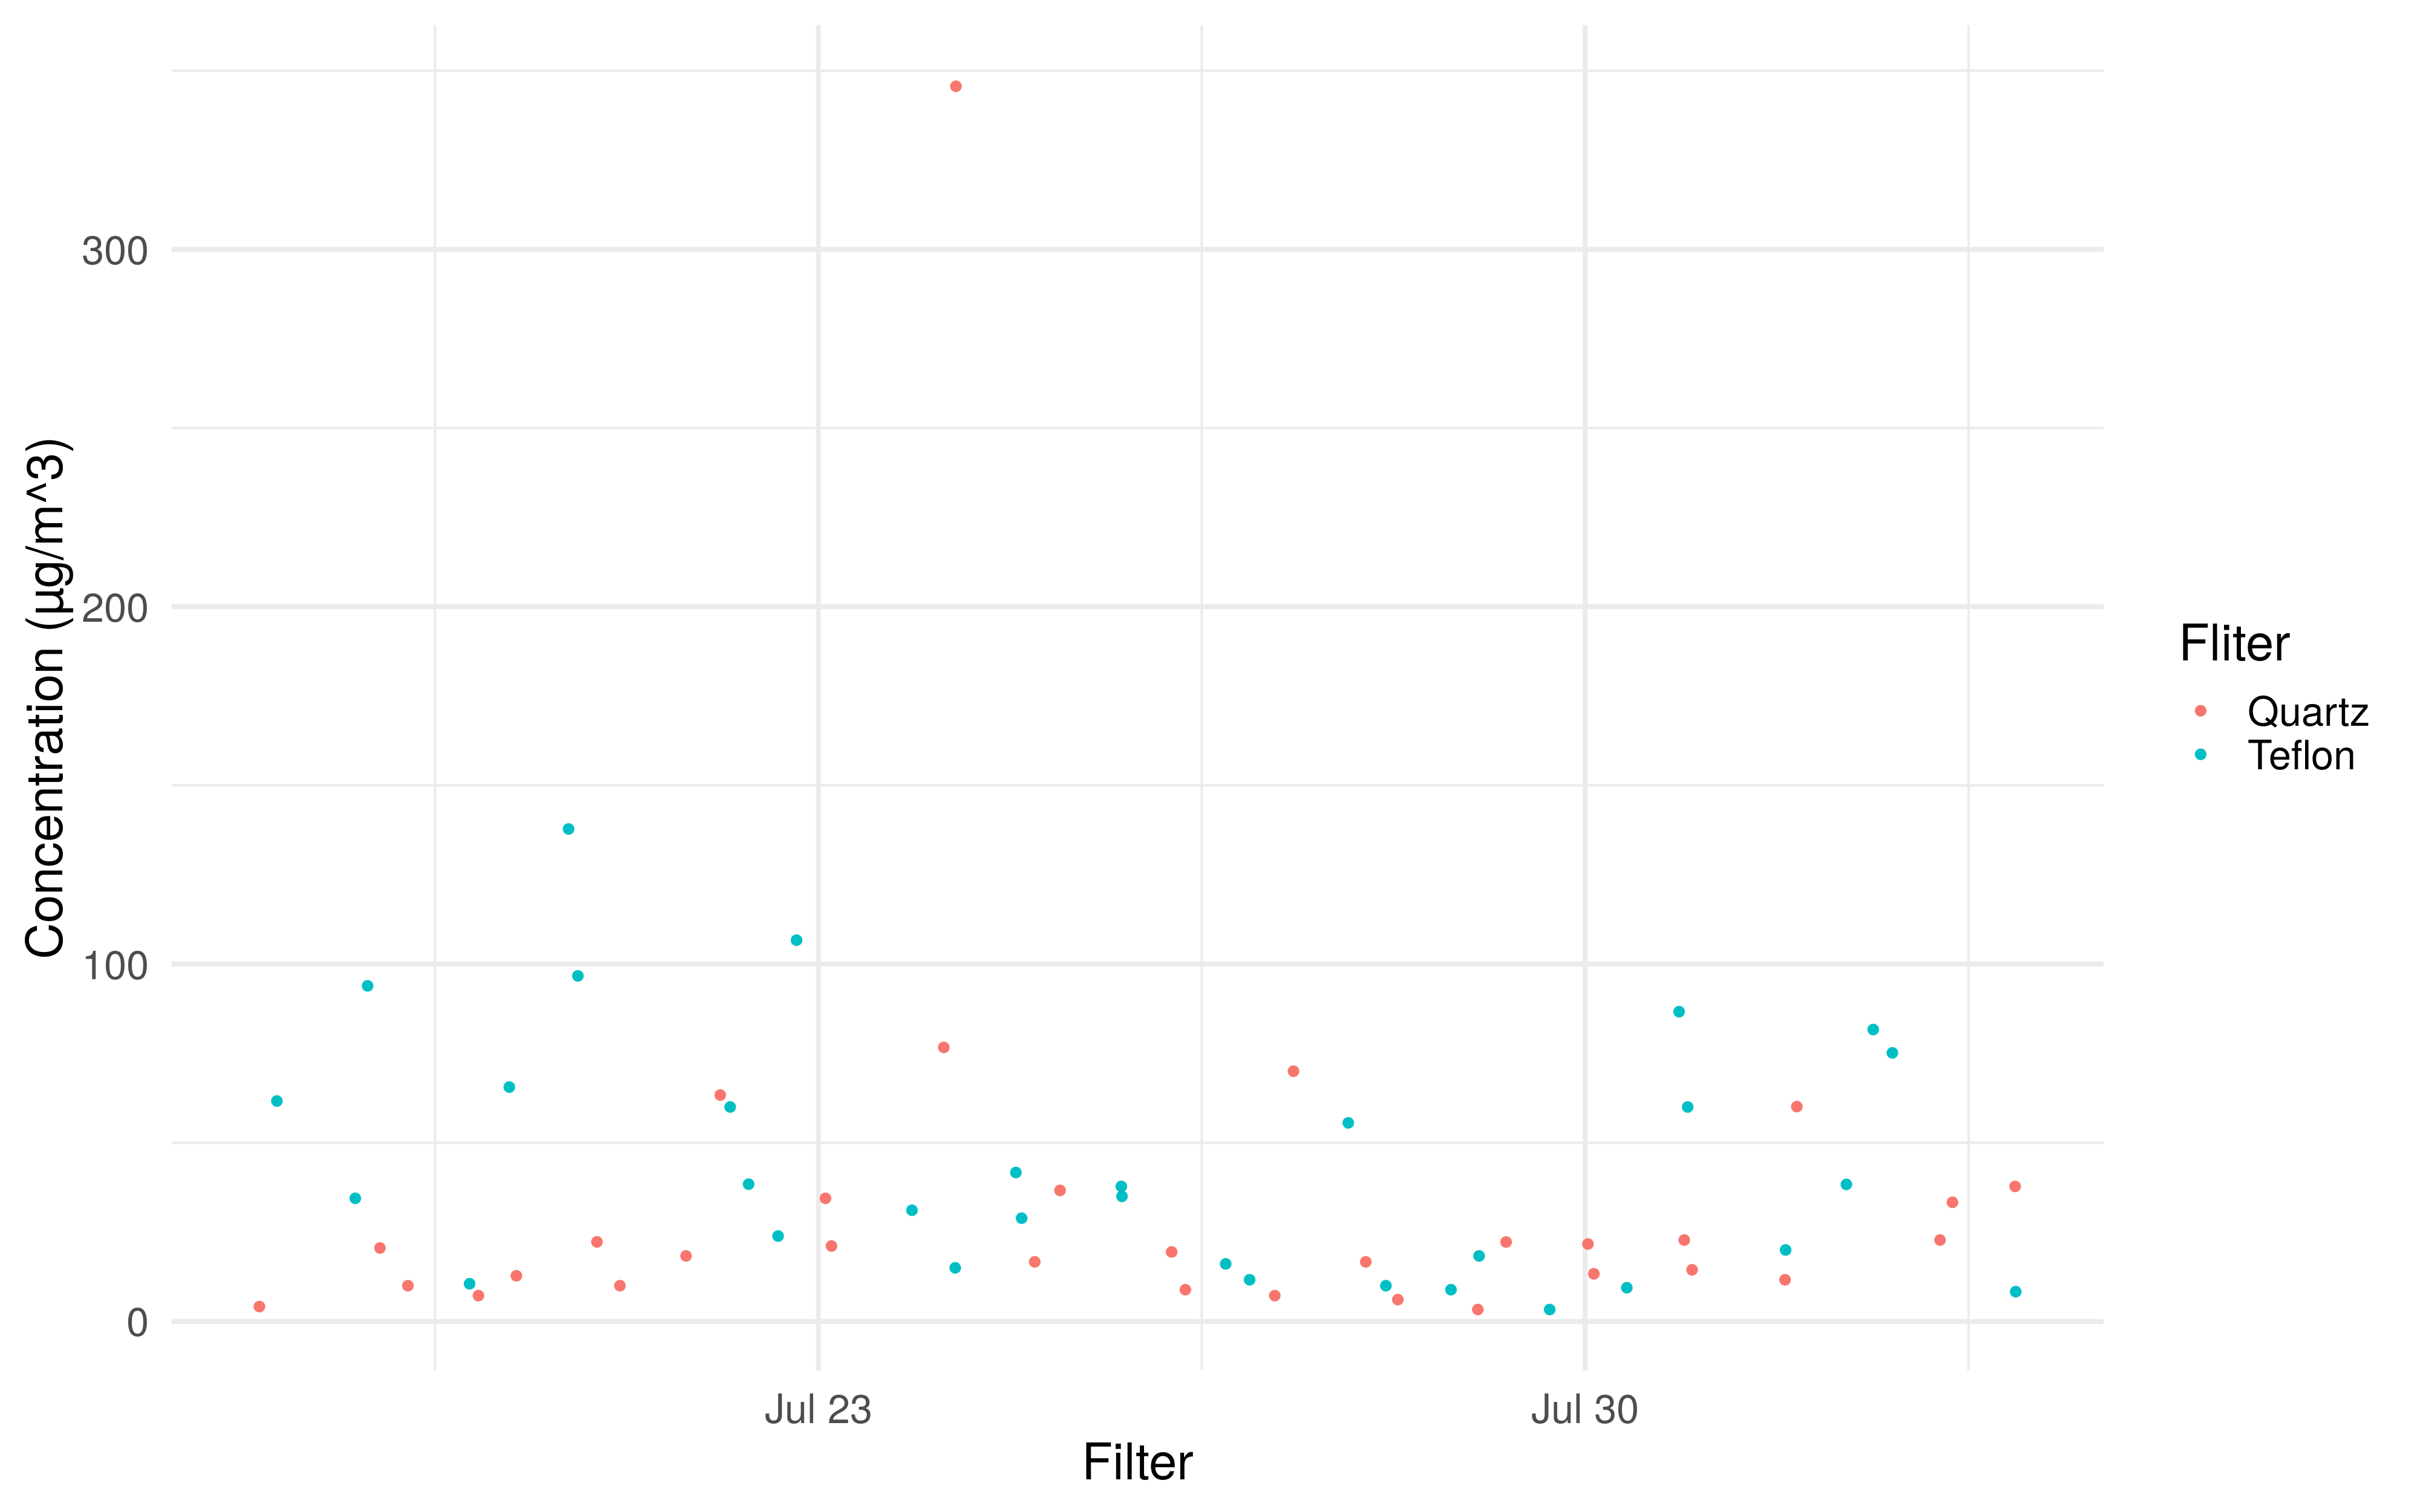
\includegraphics[width=\textwidth]{images/pm25_winter_jitter.png}
    \caption{Caption}
    \label{fig:pm2.5_winter_jitter}
\end{figure}

\begin{figure}[!htb]
    \centering
    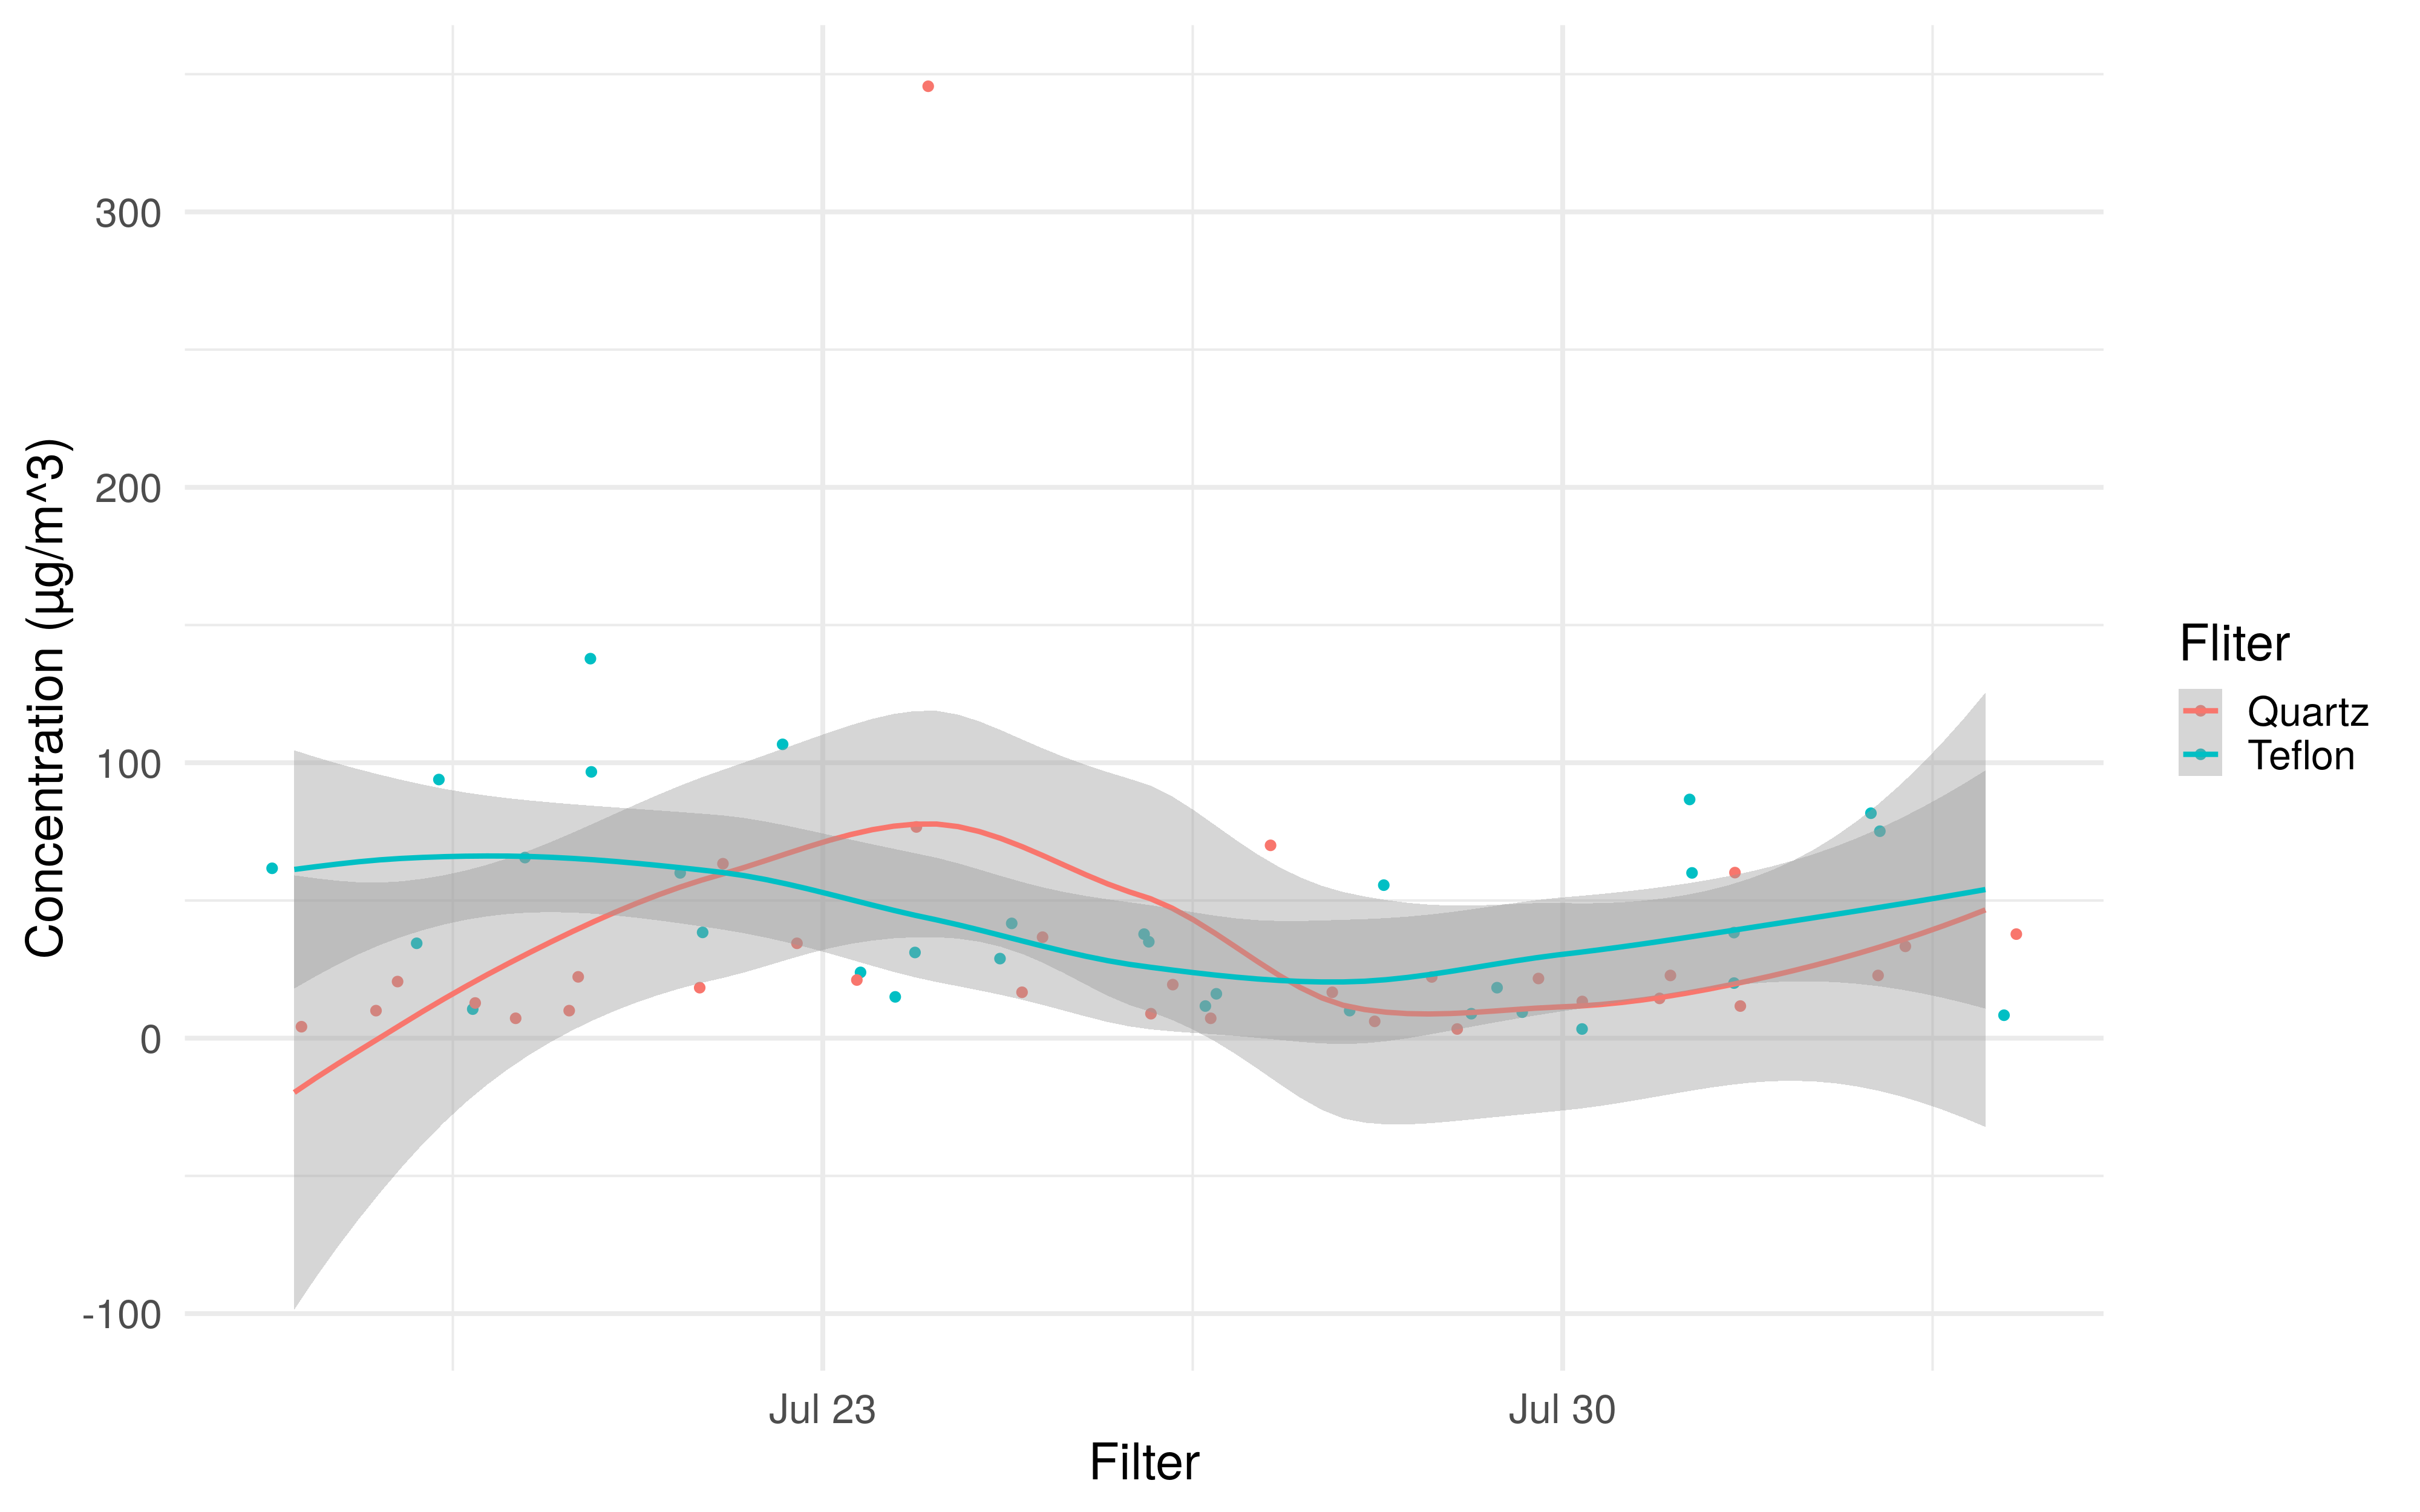
\includegraphics[width=\textwidth]{images/pm25_winter_jittersmooth.png}
    \caption{Caption}
    \label{fig:pm2.5_winter_jitter_smooth}
\end{figure}

\begin{figure}[!htb]
    \centering
    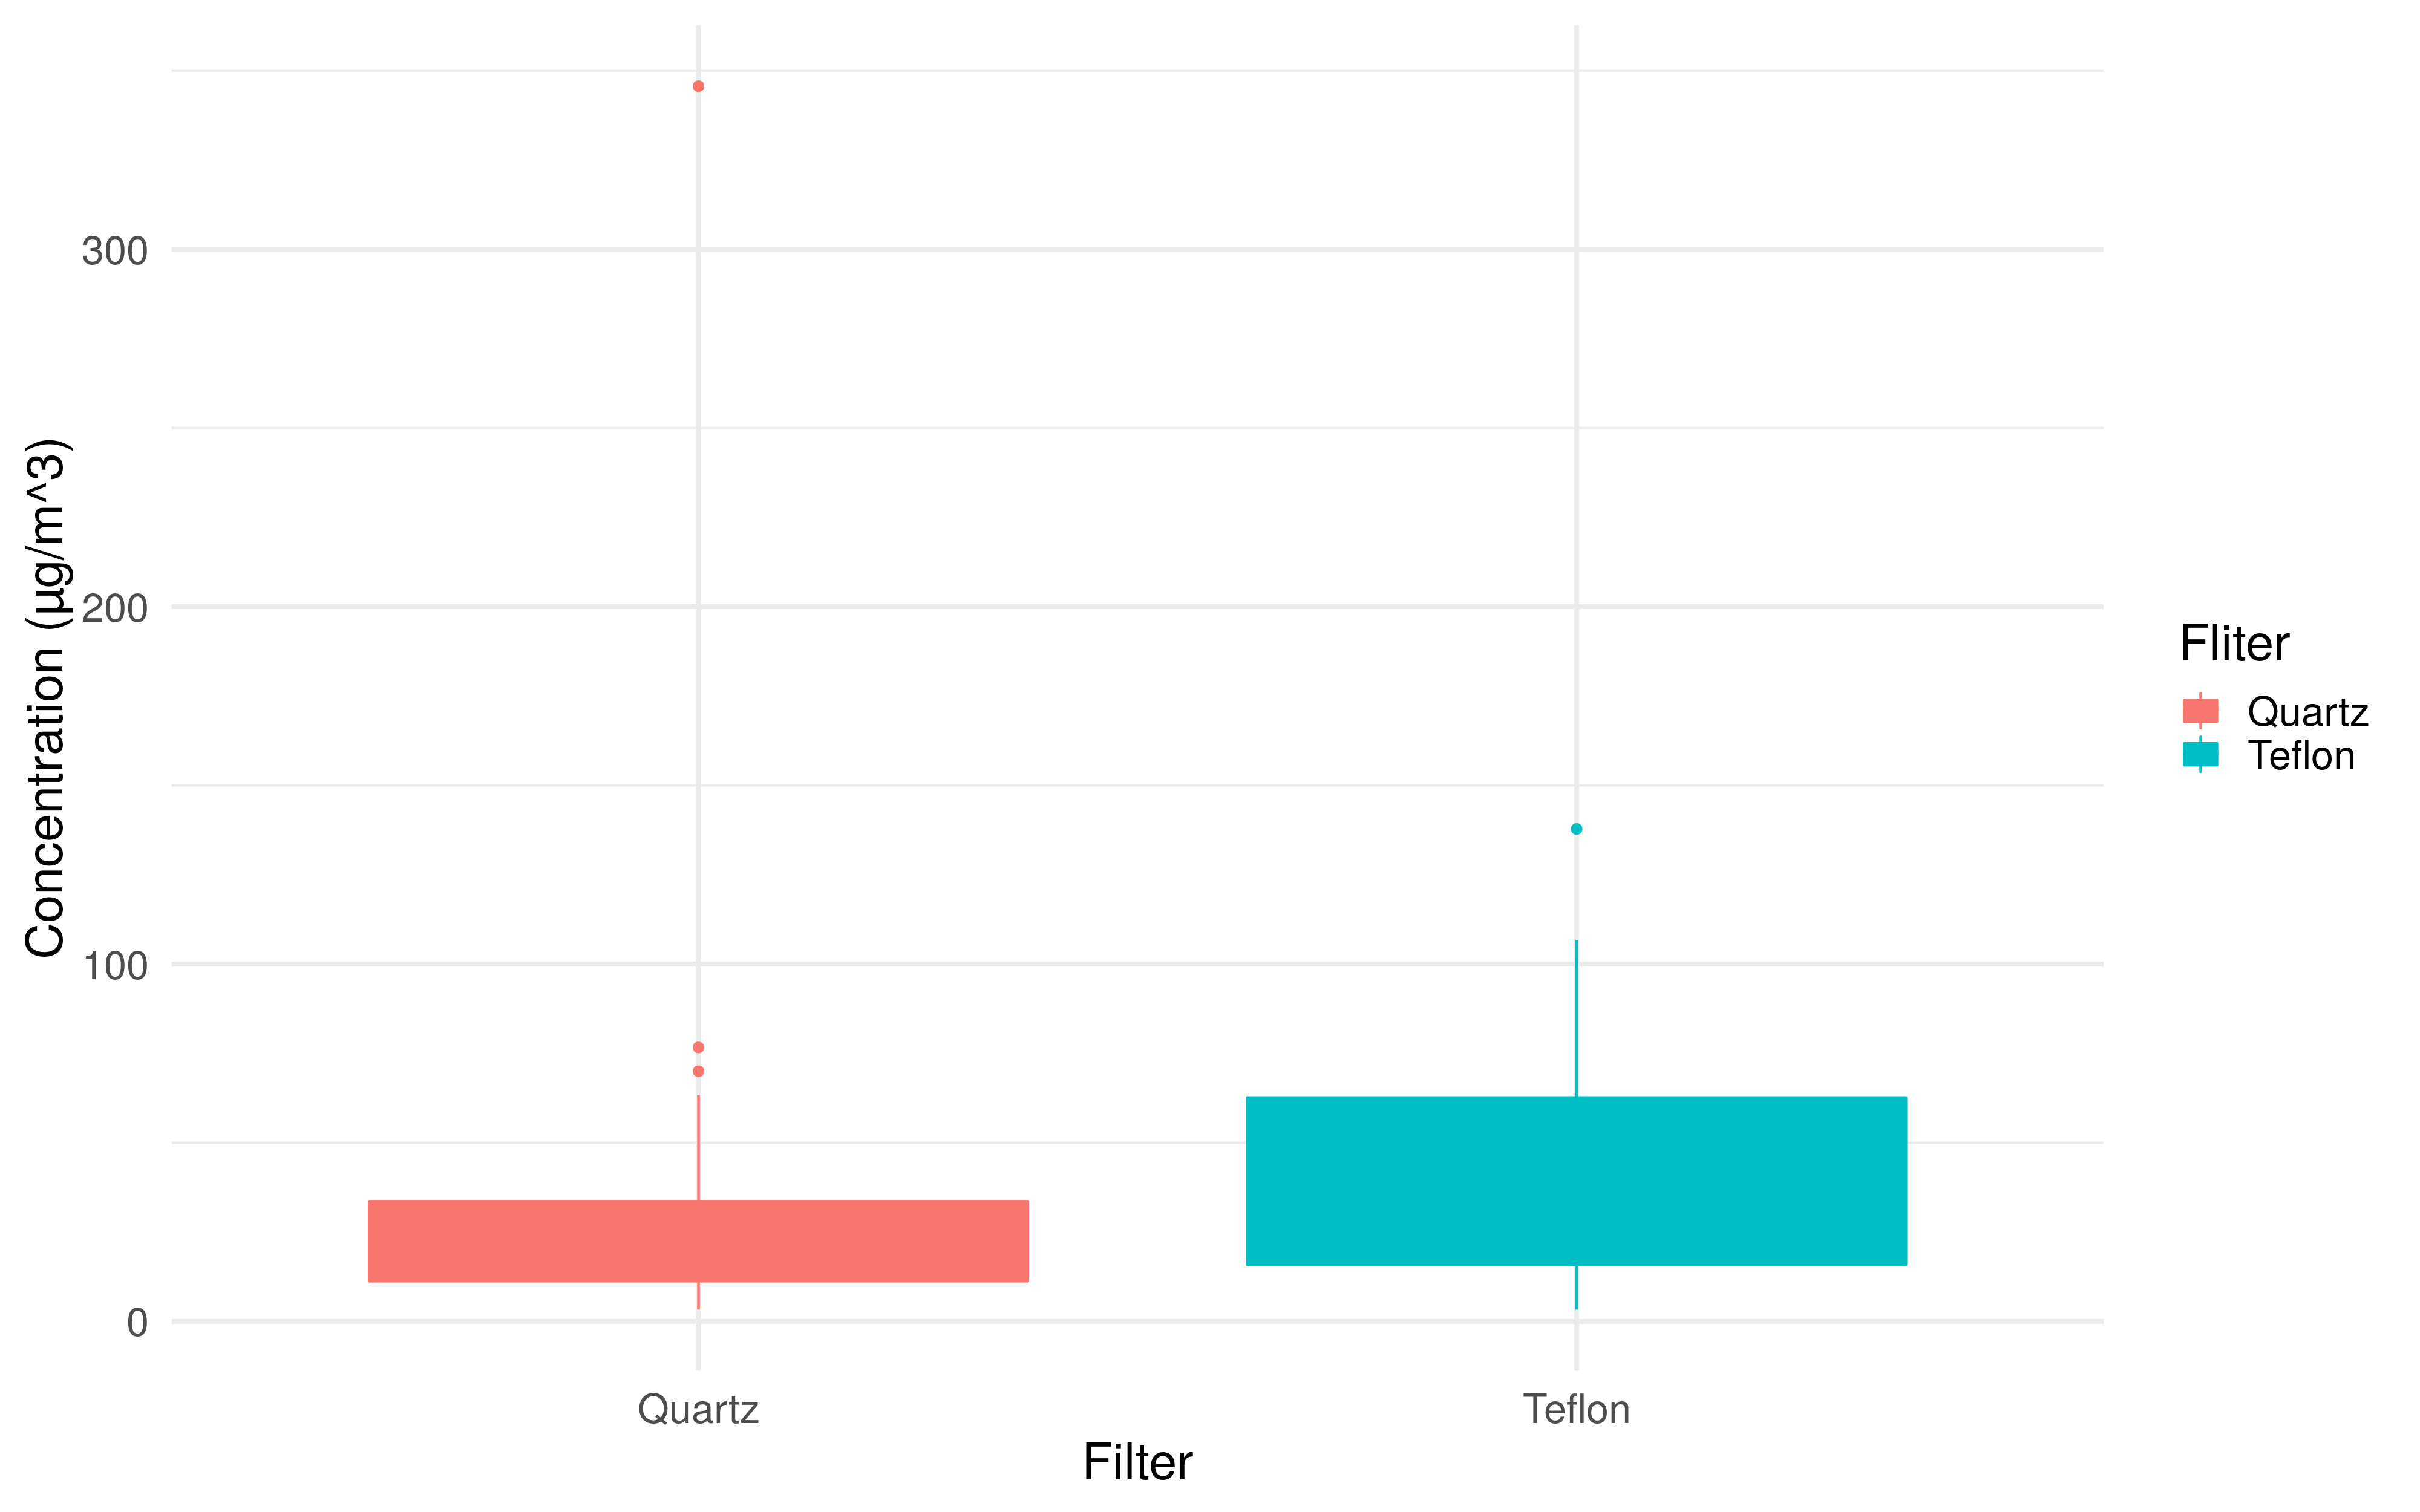
\includegraphics[width=\textwidth]{images/pm25_winter_box_filter.png}
    \caption{Caption}
    \label{fig:pm2.5_winter_box}
\end{figure}

\begin{figure}[!htb]
    \centering
    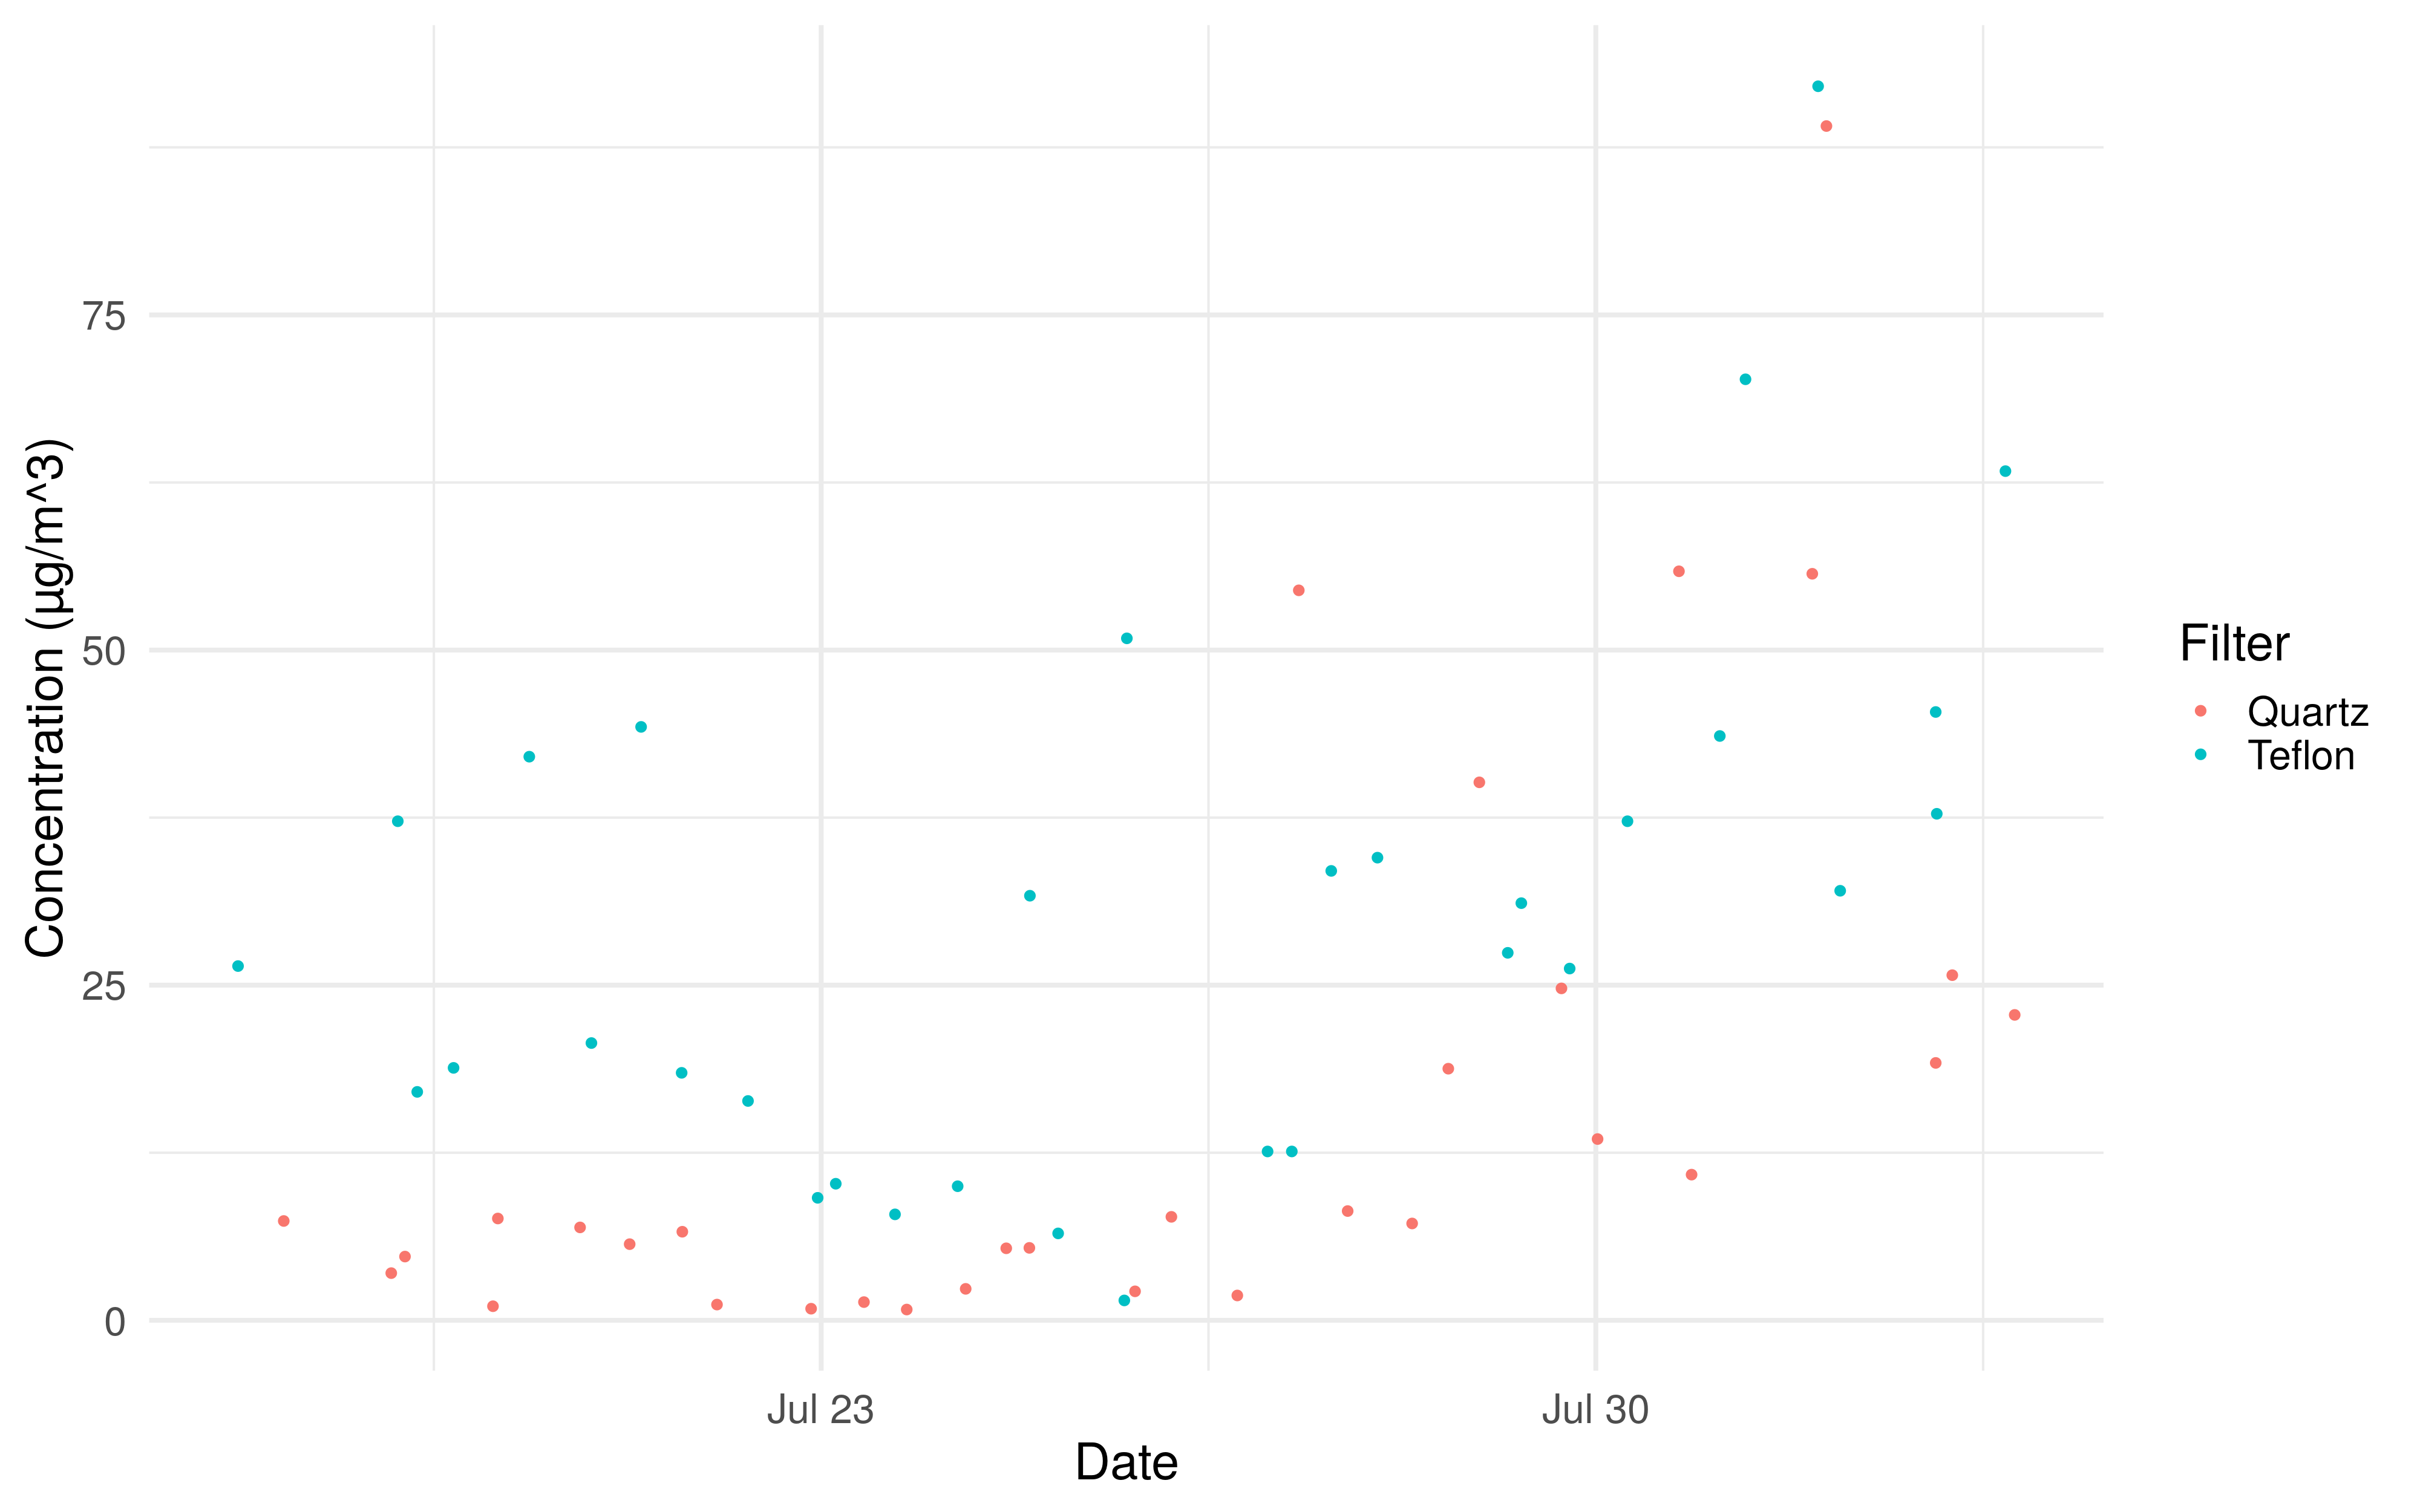
\includegraphics[width=\textwidth]{images/pm10_winter_jitter.png}
    \caption{Caption}
    \label{fig:pm10_winter_jitter}
\end{figure}

\begin{figure}[!htb]
    \centering
    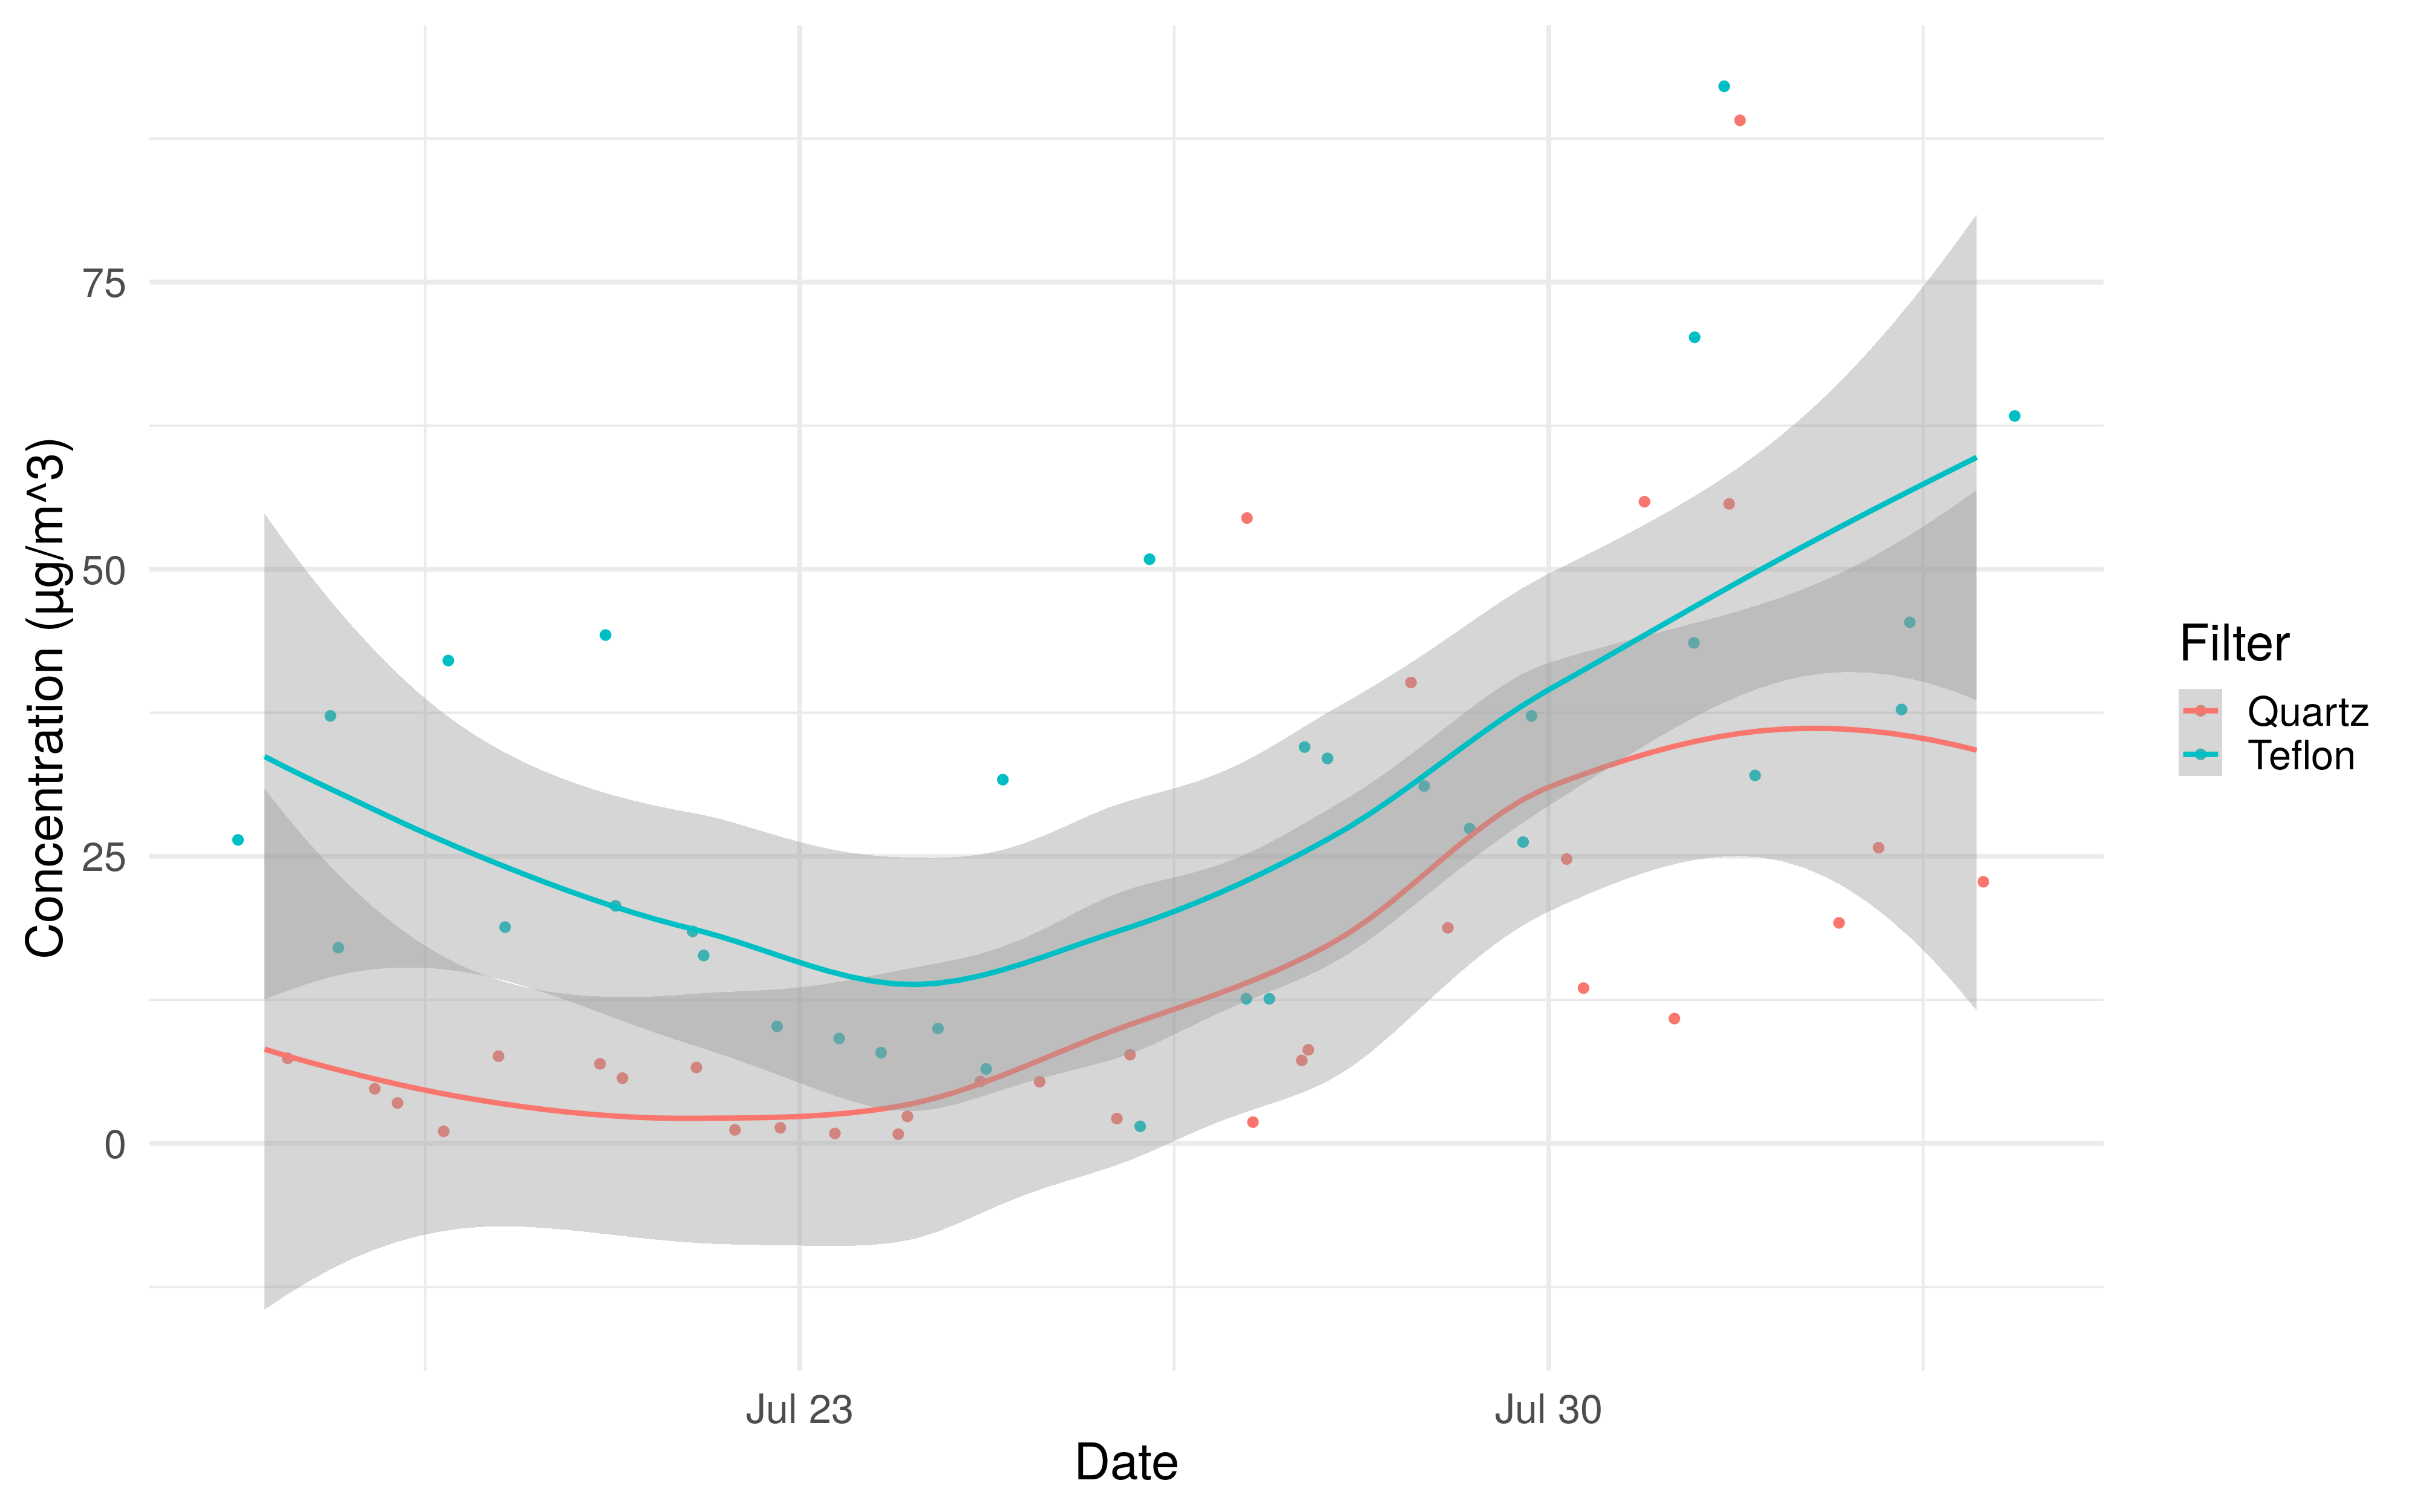
\includegraphics[width=\textwidth]{images/pm10_winter_jittersmooth.png}
    \caption{Caption}
    \label{fig:pm10_winter_jitter_smooth}
\end{figure}

\begin{figure}[!htb]
    \centering
    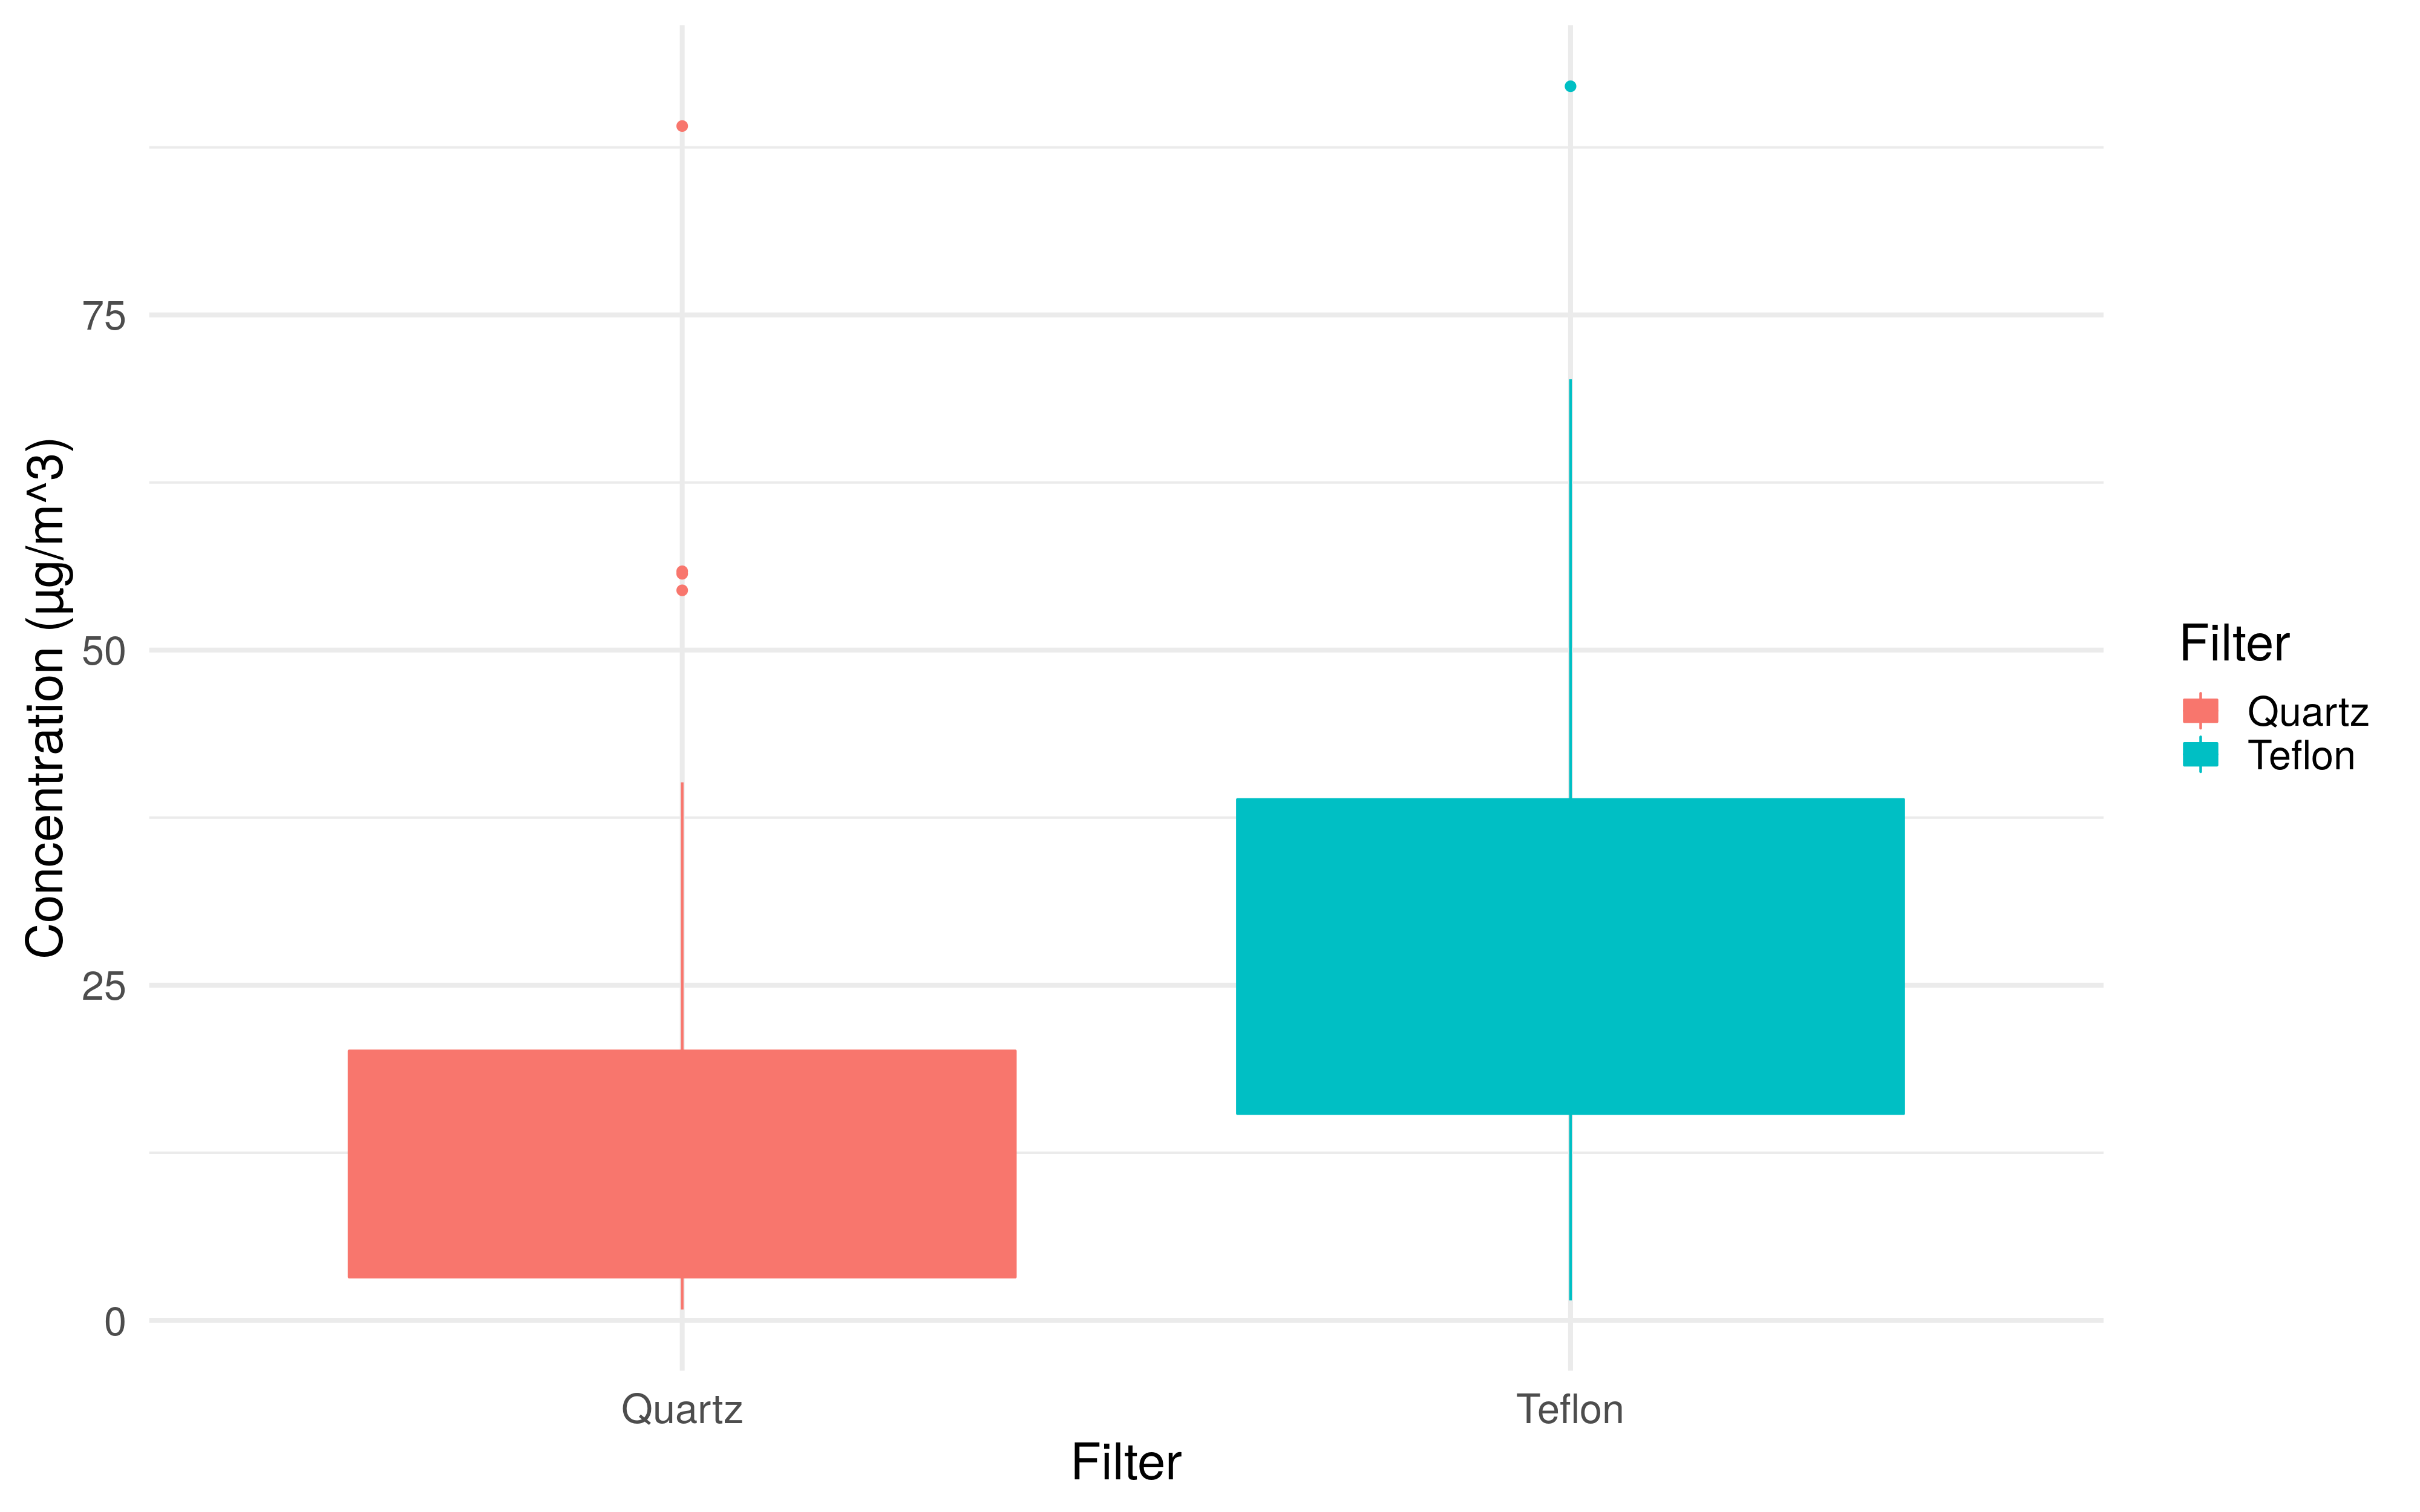
\includegraphics[width=\textwidth]{images/pm10_winter_box_filter.png}
    \caption{Caption}
    \label{fig:pm10_winter_box}
\end{figure}

%%%%%%%%%%%%%%%%%%%%%%%%%%%%%%%%%%%%%%%%%%%%%%%%%%%%%%%%%%%%%%%%

\begin{figure}[!htb]
    \centering
    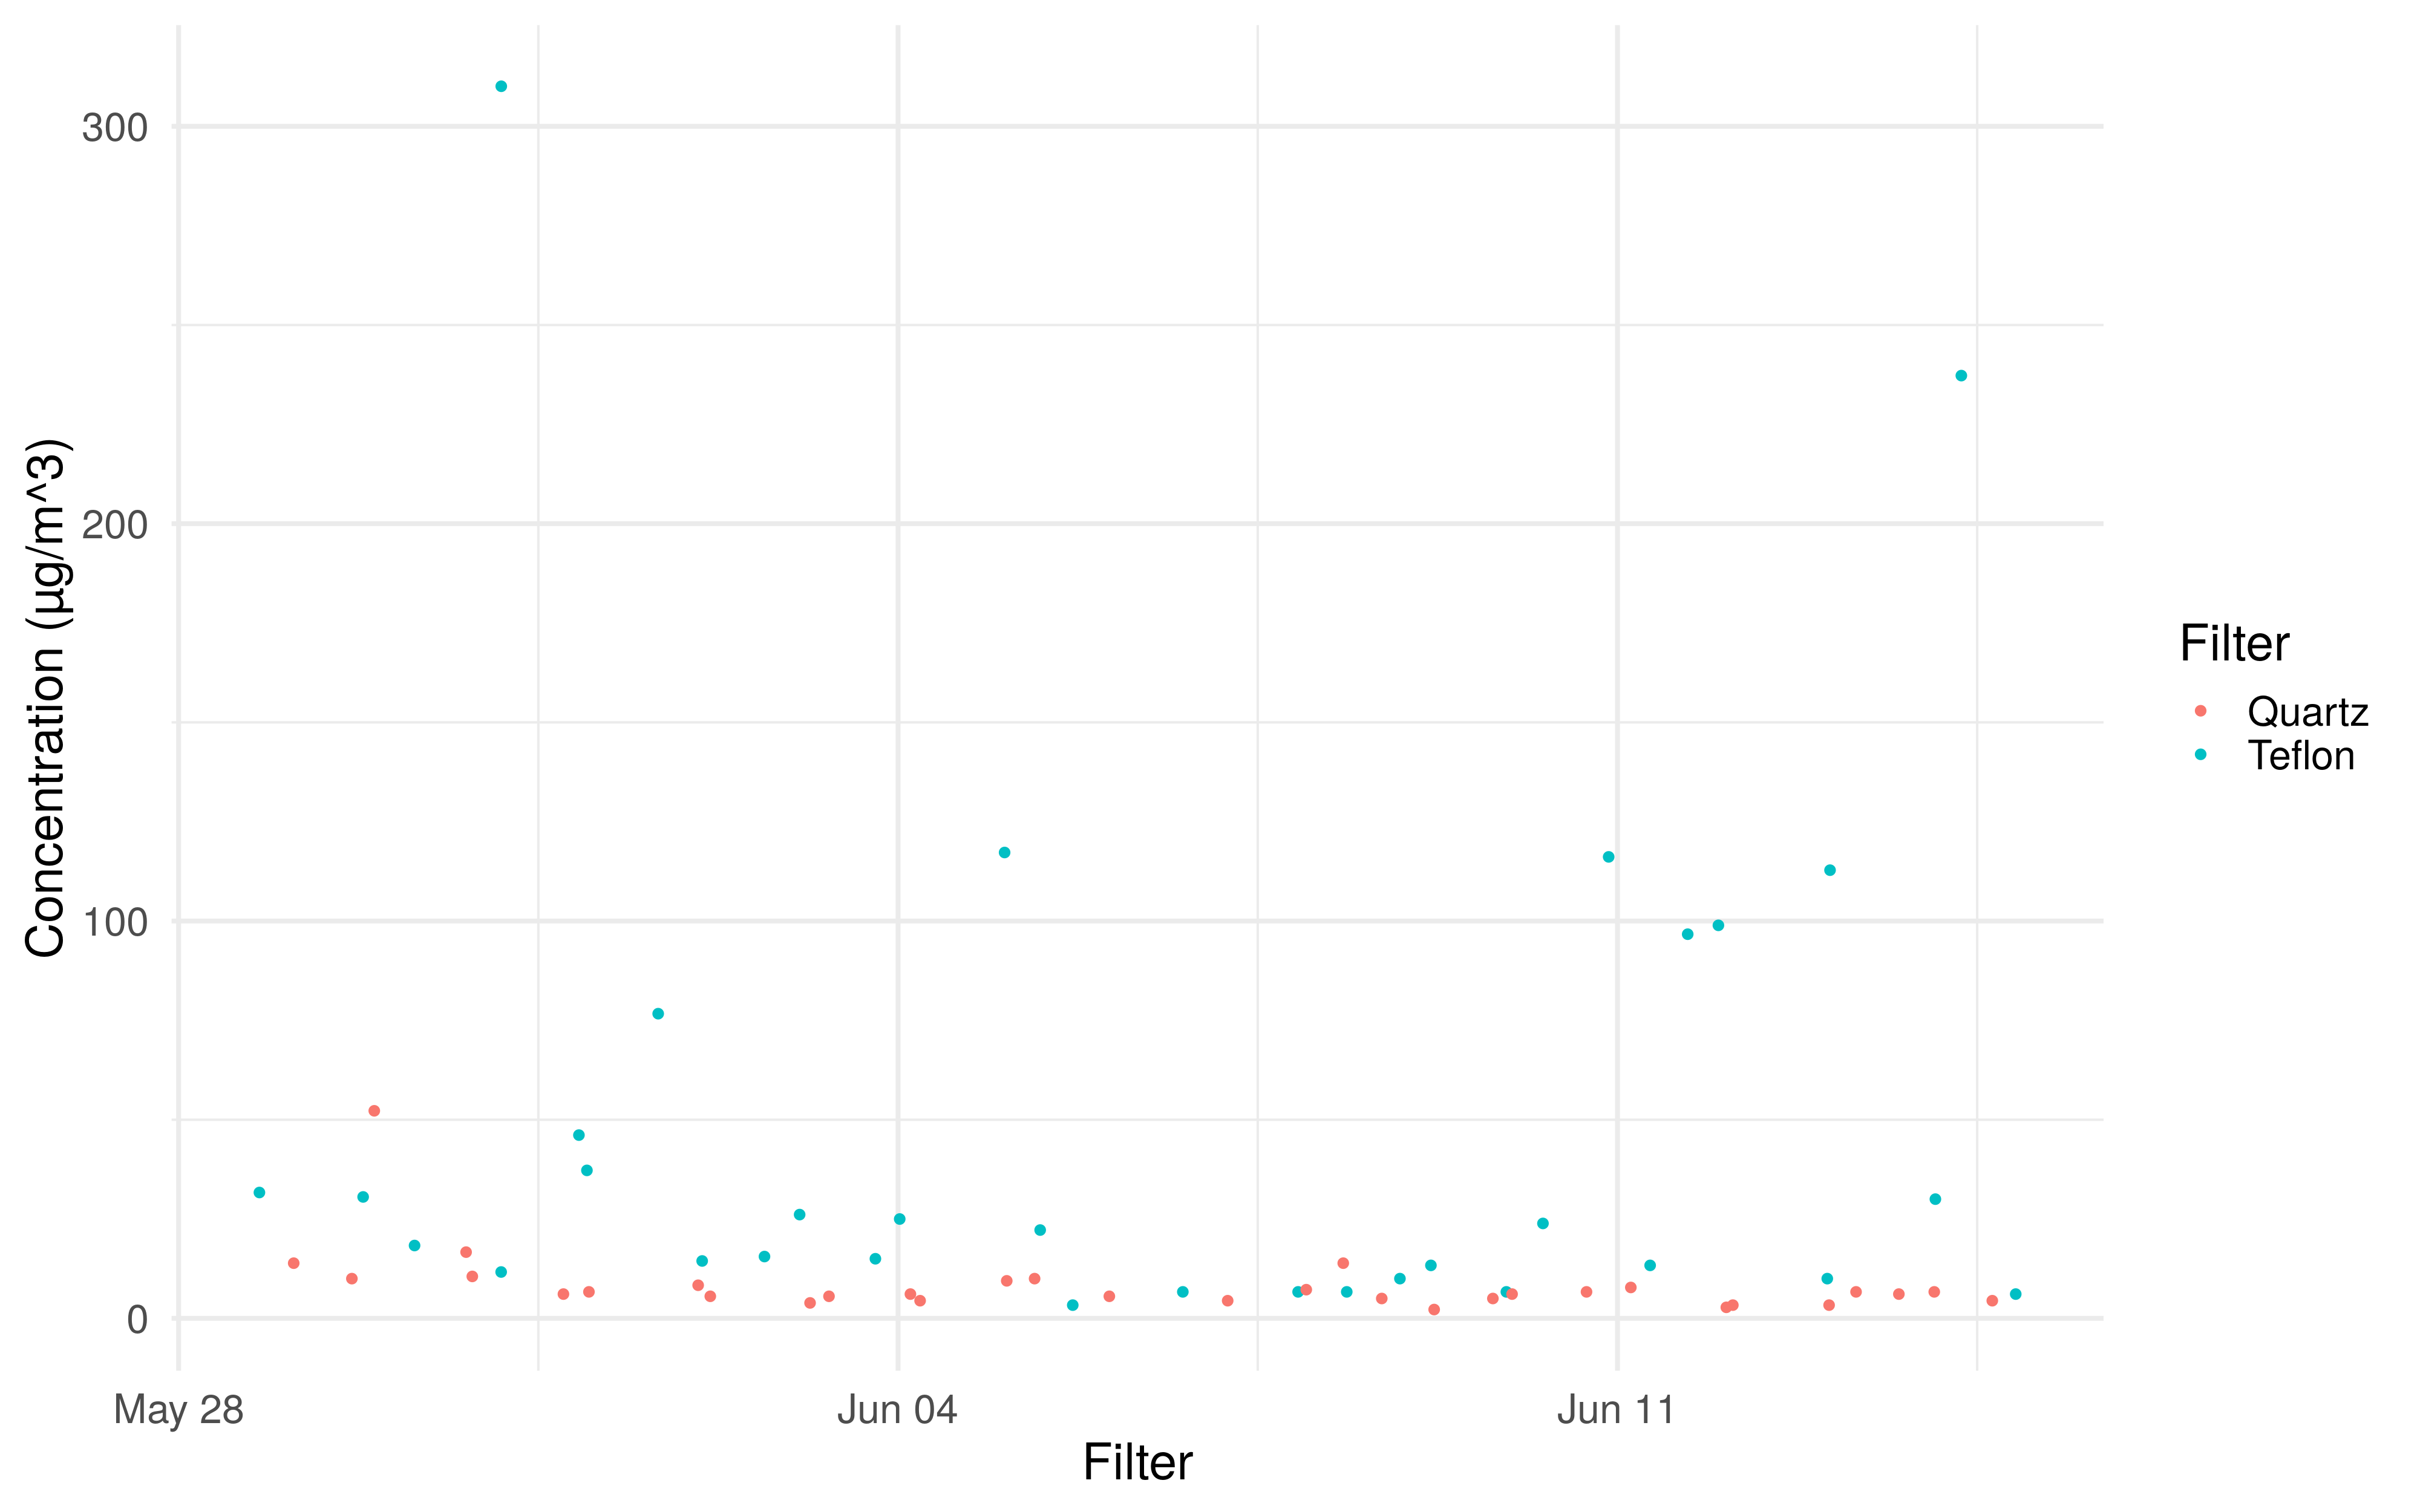
\includegraphics[width=\textwidth]{images/pm25_autumn_jitter.png}
    \caption{Caption}
    \label{fig:pm2.5_autumn_jitter}
\end{figure}

\begin{figure}[!htb]
    \centering
    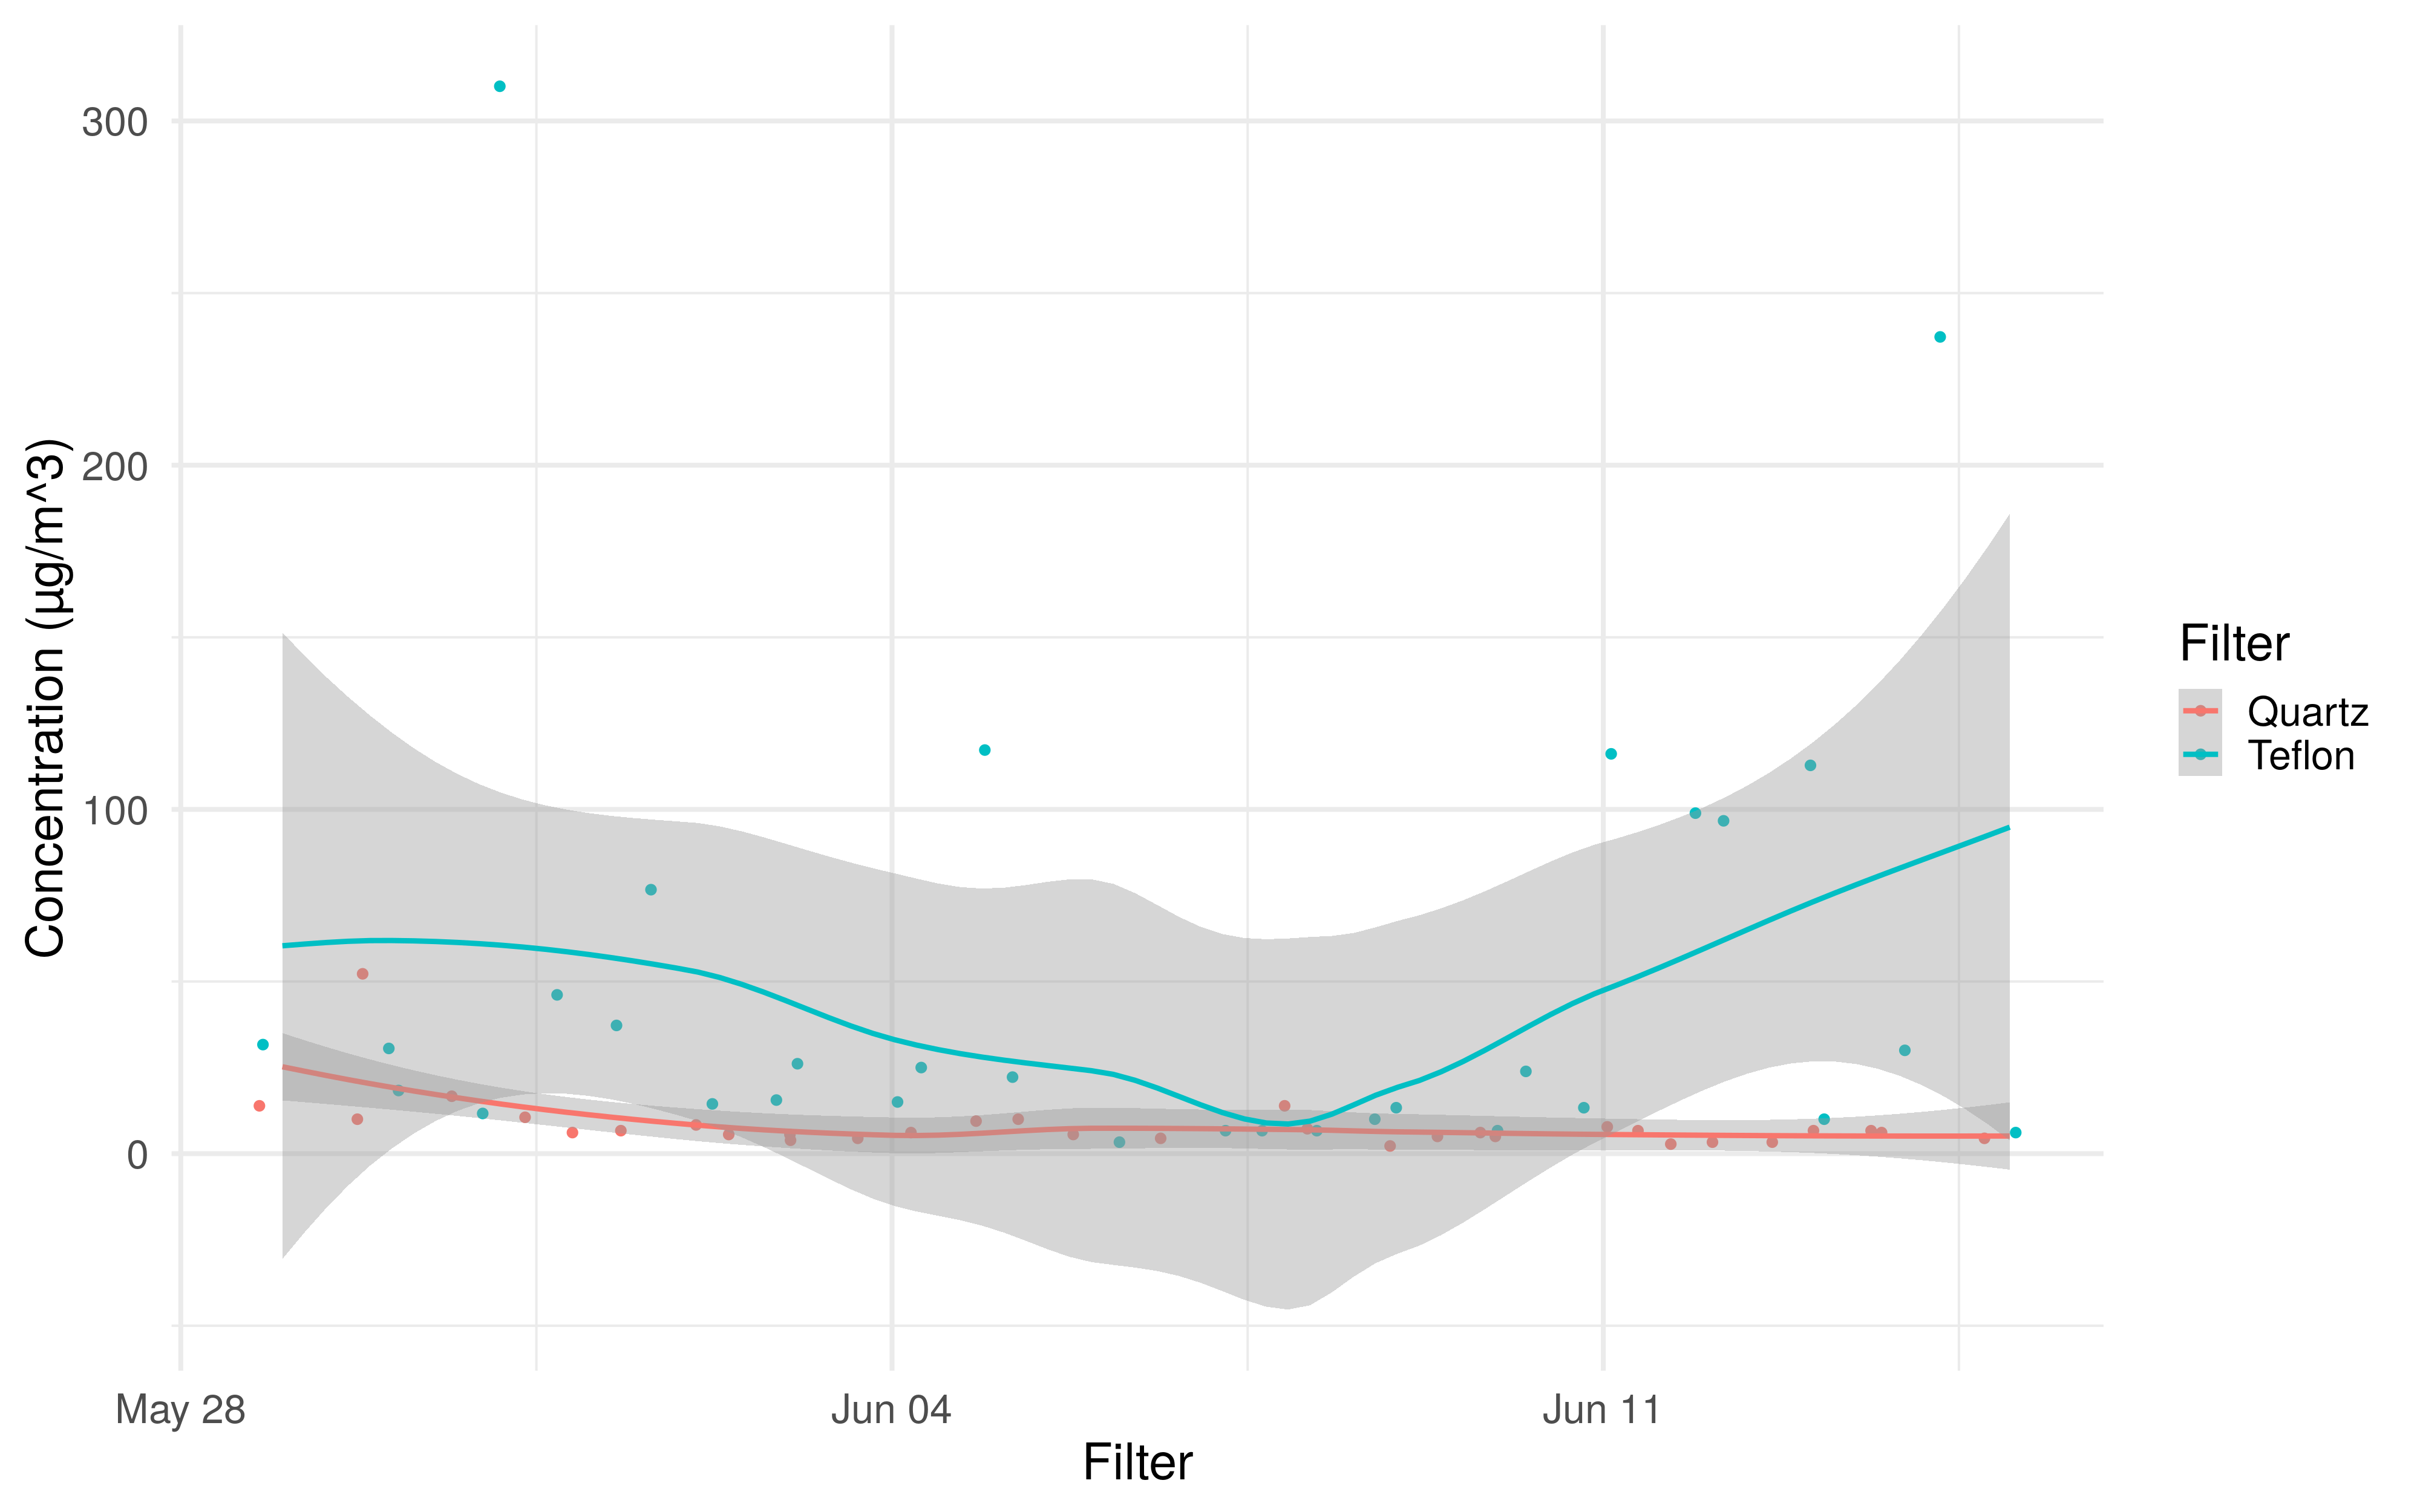
\includegraphics[width=\textwidth]{images/pm25_autumn_jittersmooth.png}
    \caption{Caption}
    \label{fig:pm2.5_autumn_jitter_smooth}
\end{figure}

\begin{figure}[!htb]
    \centering
    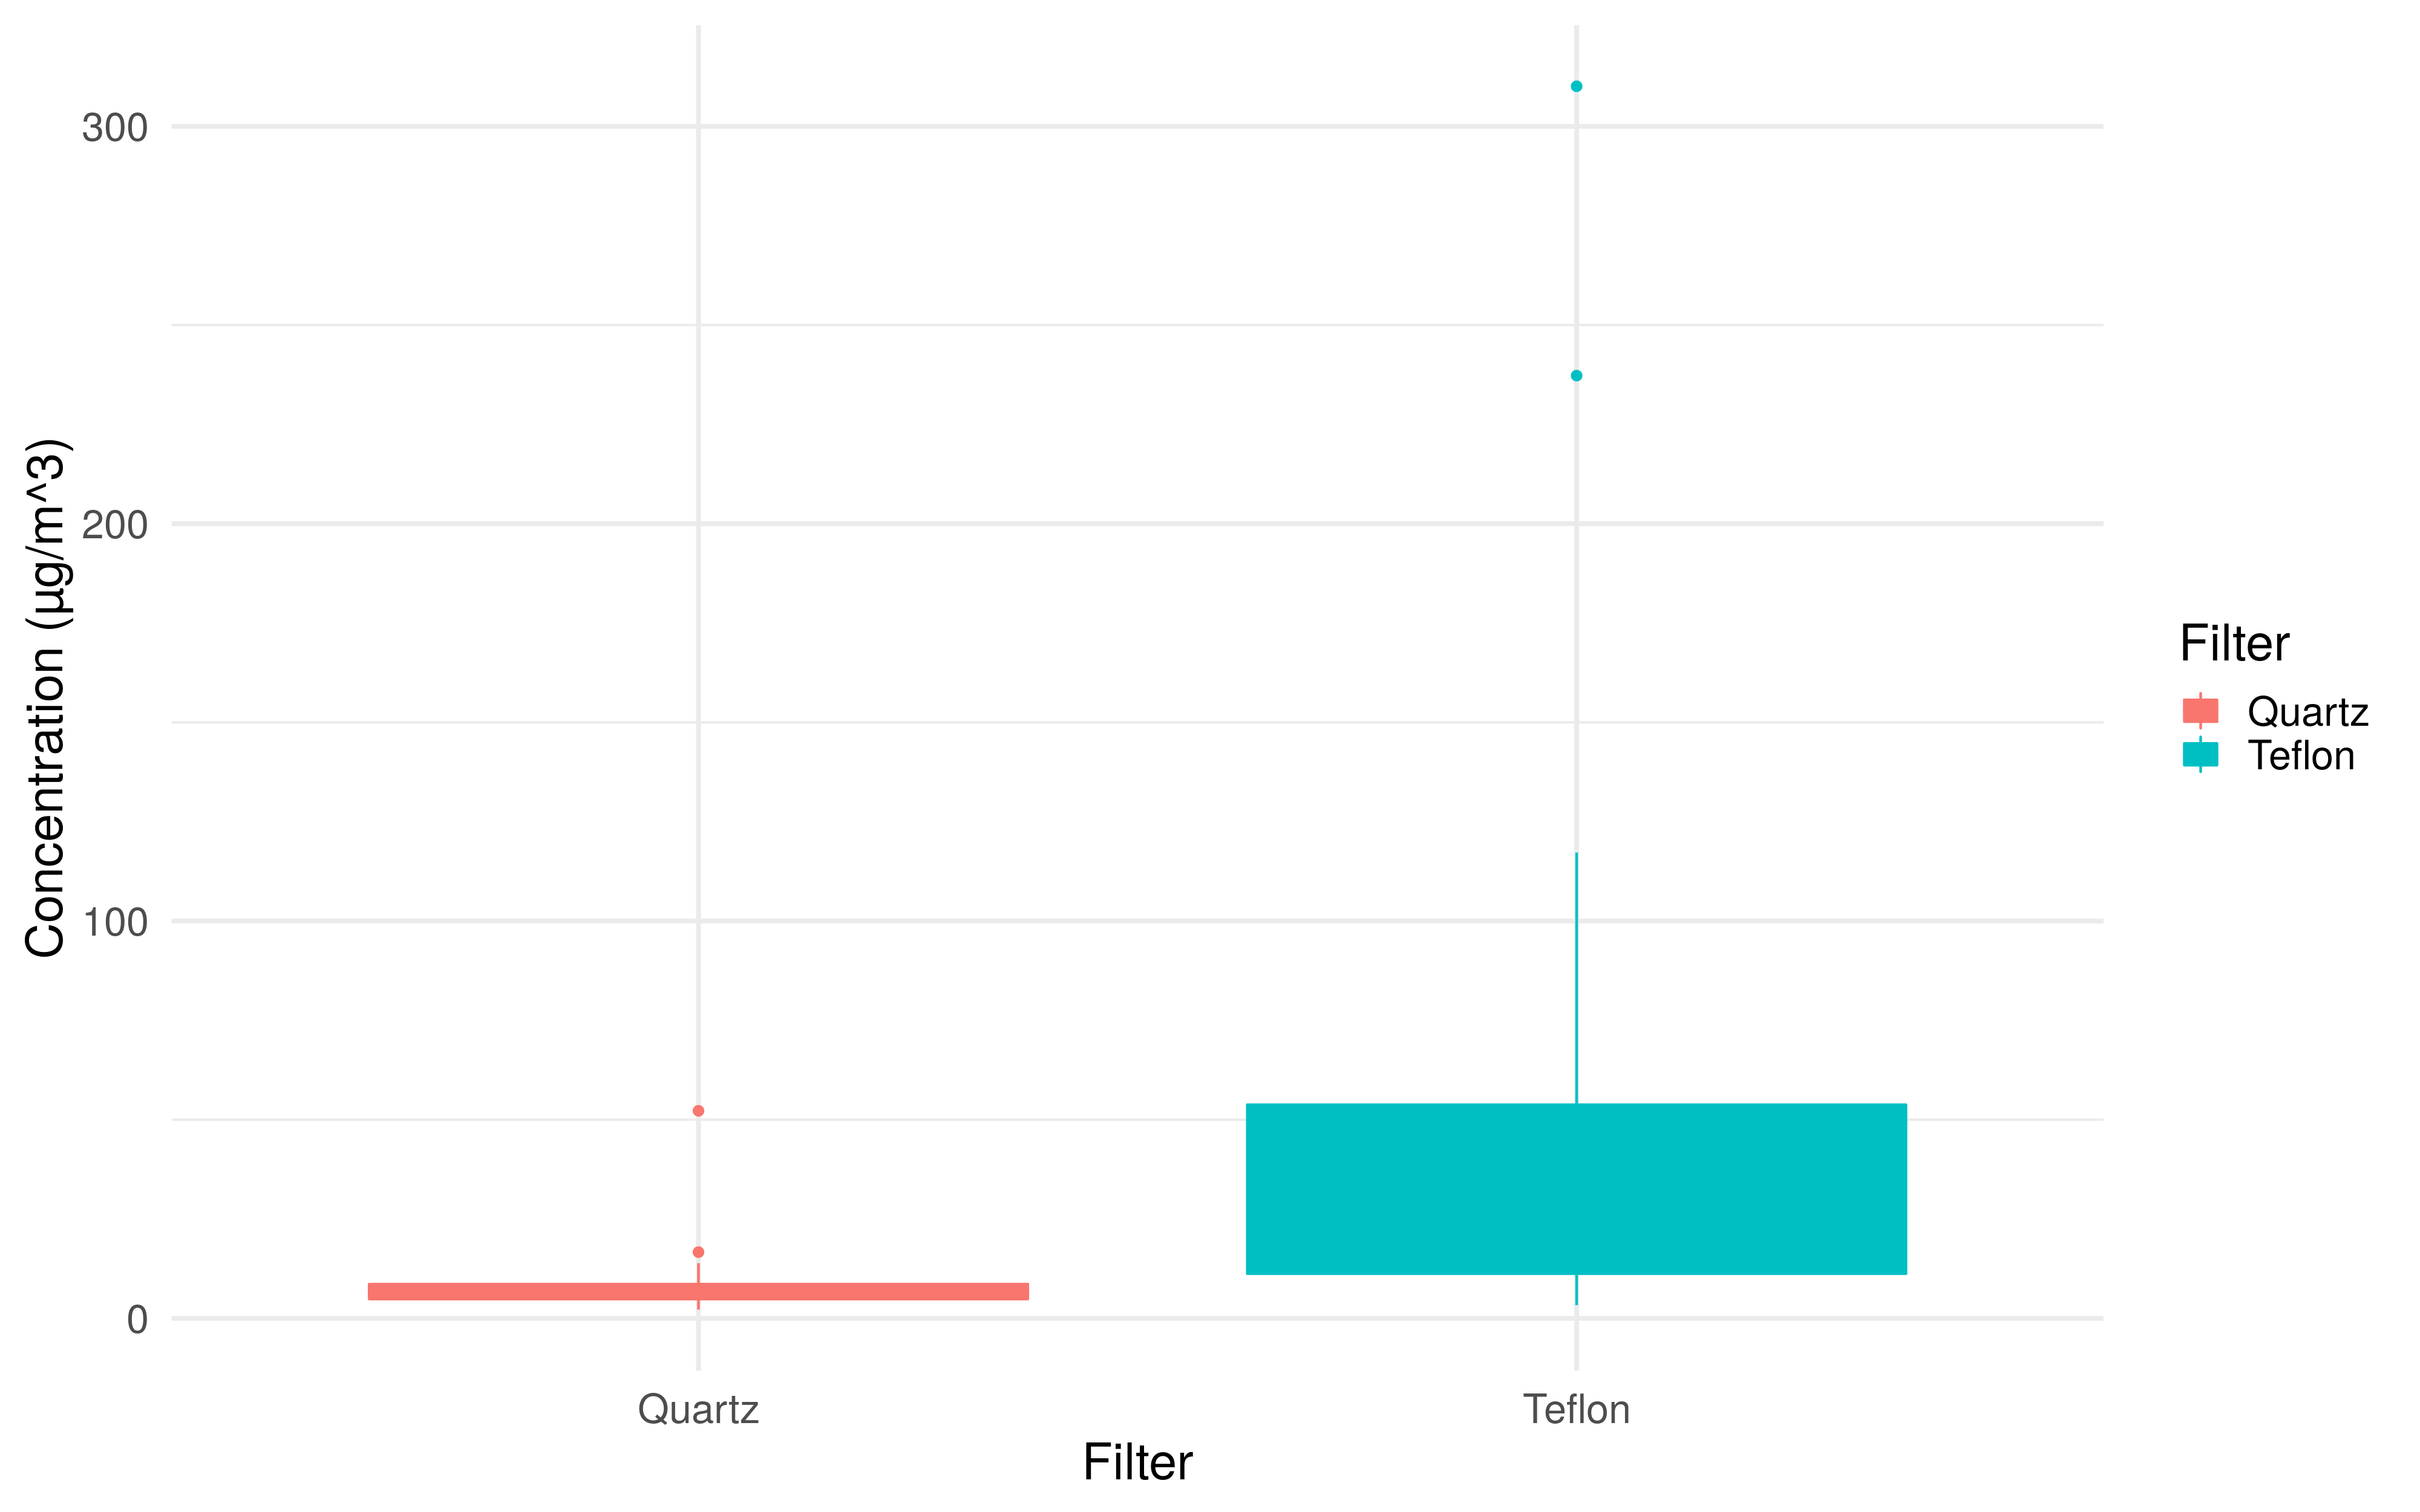
\includegraphics[width=\textwidth]{images/pm25_autumn_box.png}
    \caption{Caption}
    \label{fig:pm2.5_autumn_box}
\end{figure}

\begin{figure}[!htb]
    \centering
    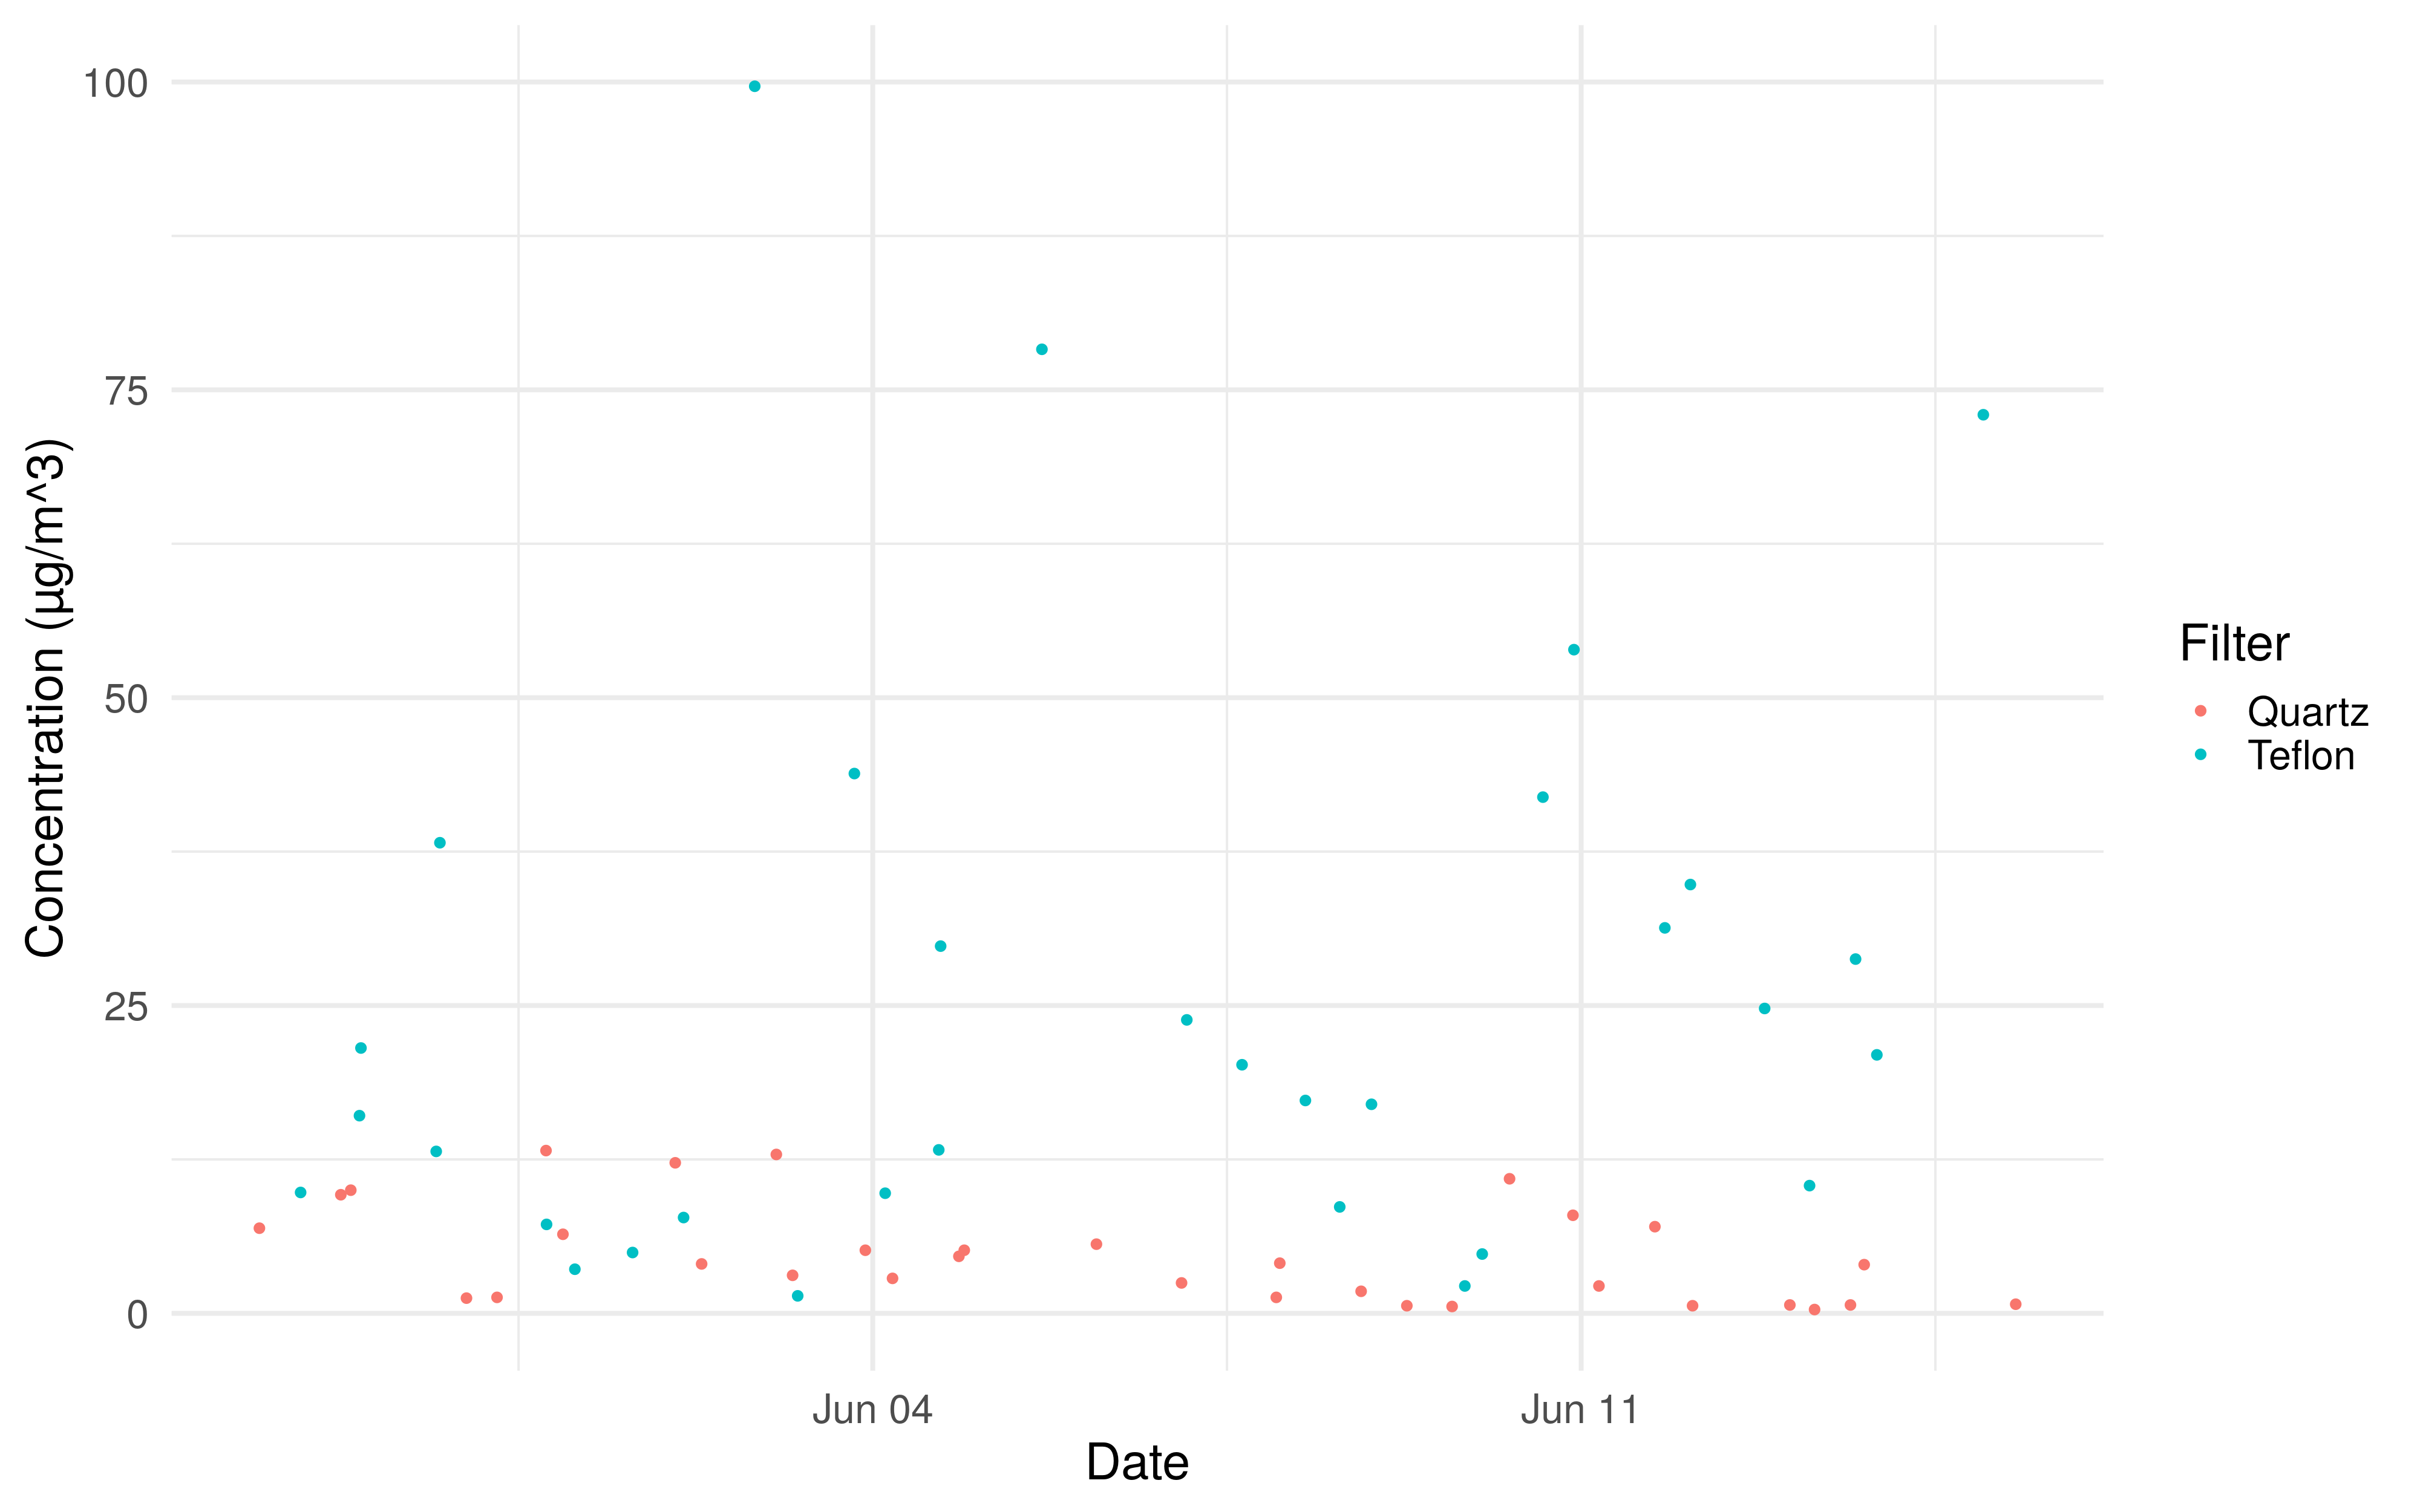
\includegraphics[width=\textwidth]{images/pm10_autumn_jitter.png}
    \caption{Caption}
    \label{fig:pm10_autumn_jitter}
\end{figure}

\begin{figure}[!htb]
    \centering
    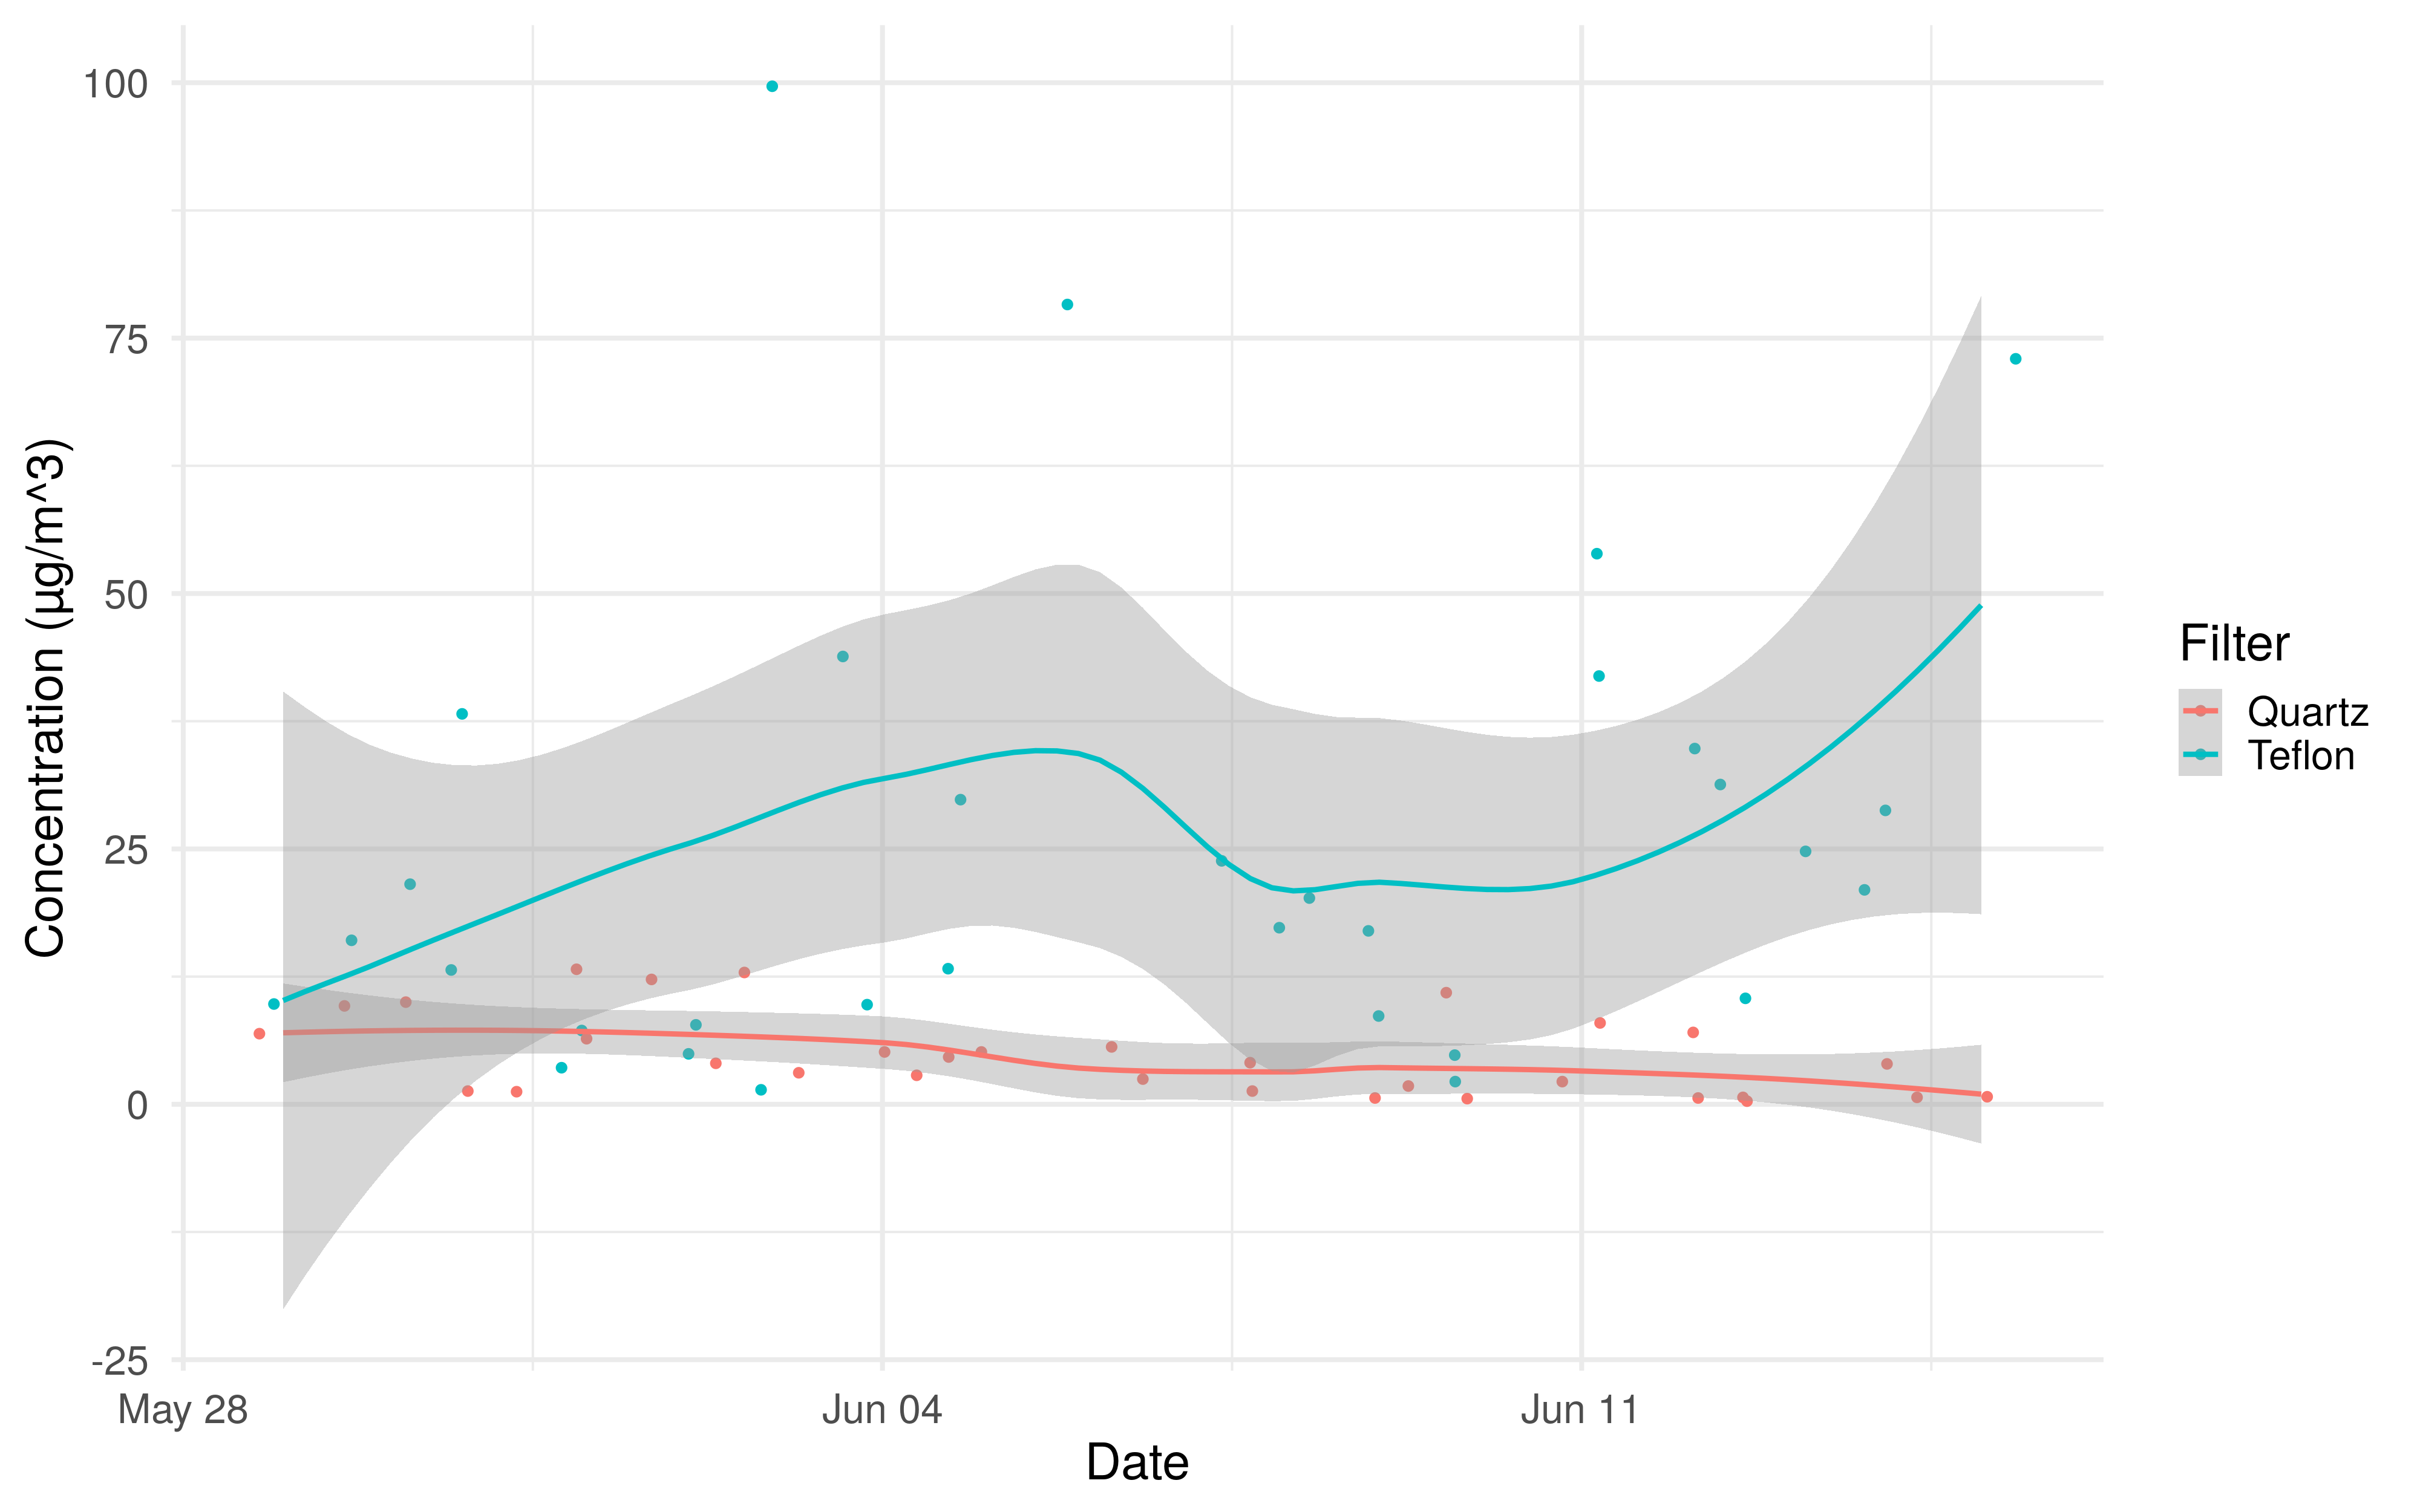
\includegraphics[width=\textwidth]{images/pm10_autumn_jittersmooth.png}
    \caption{Caption}
    \label{fig:pm10_autumn_jitter_smooth}
\end{figure}

\begin{figure}[!htb]
    \centering
    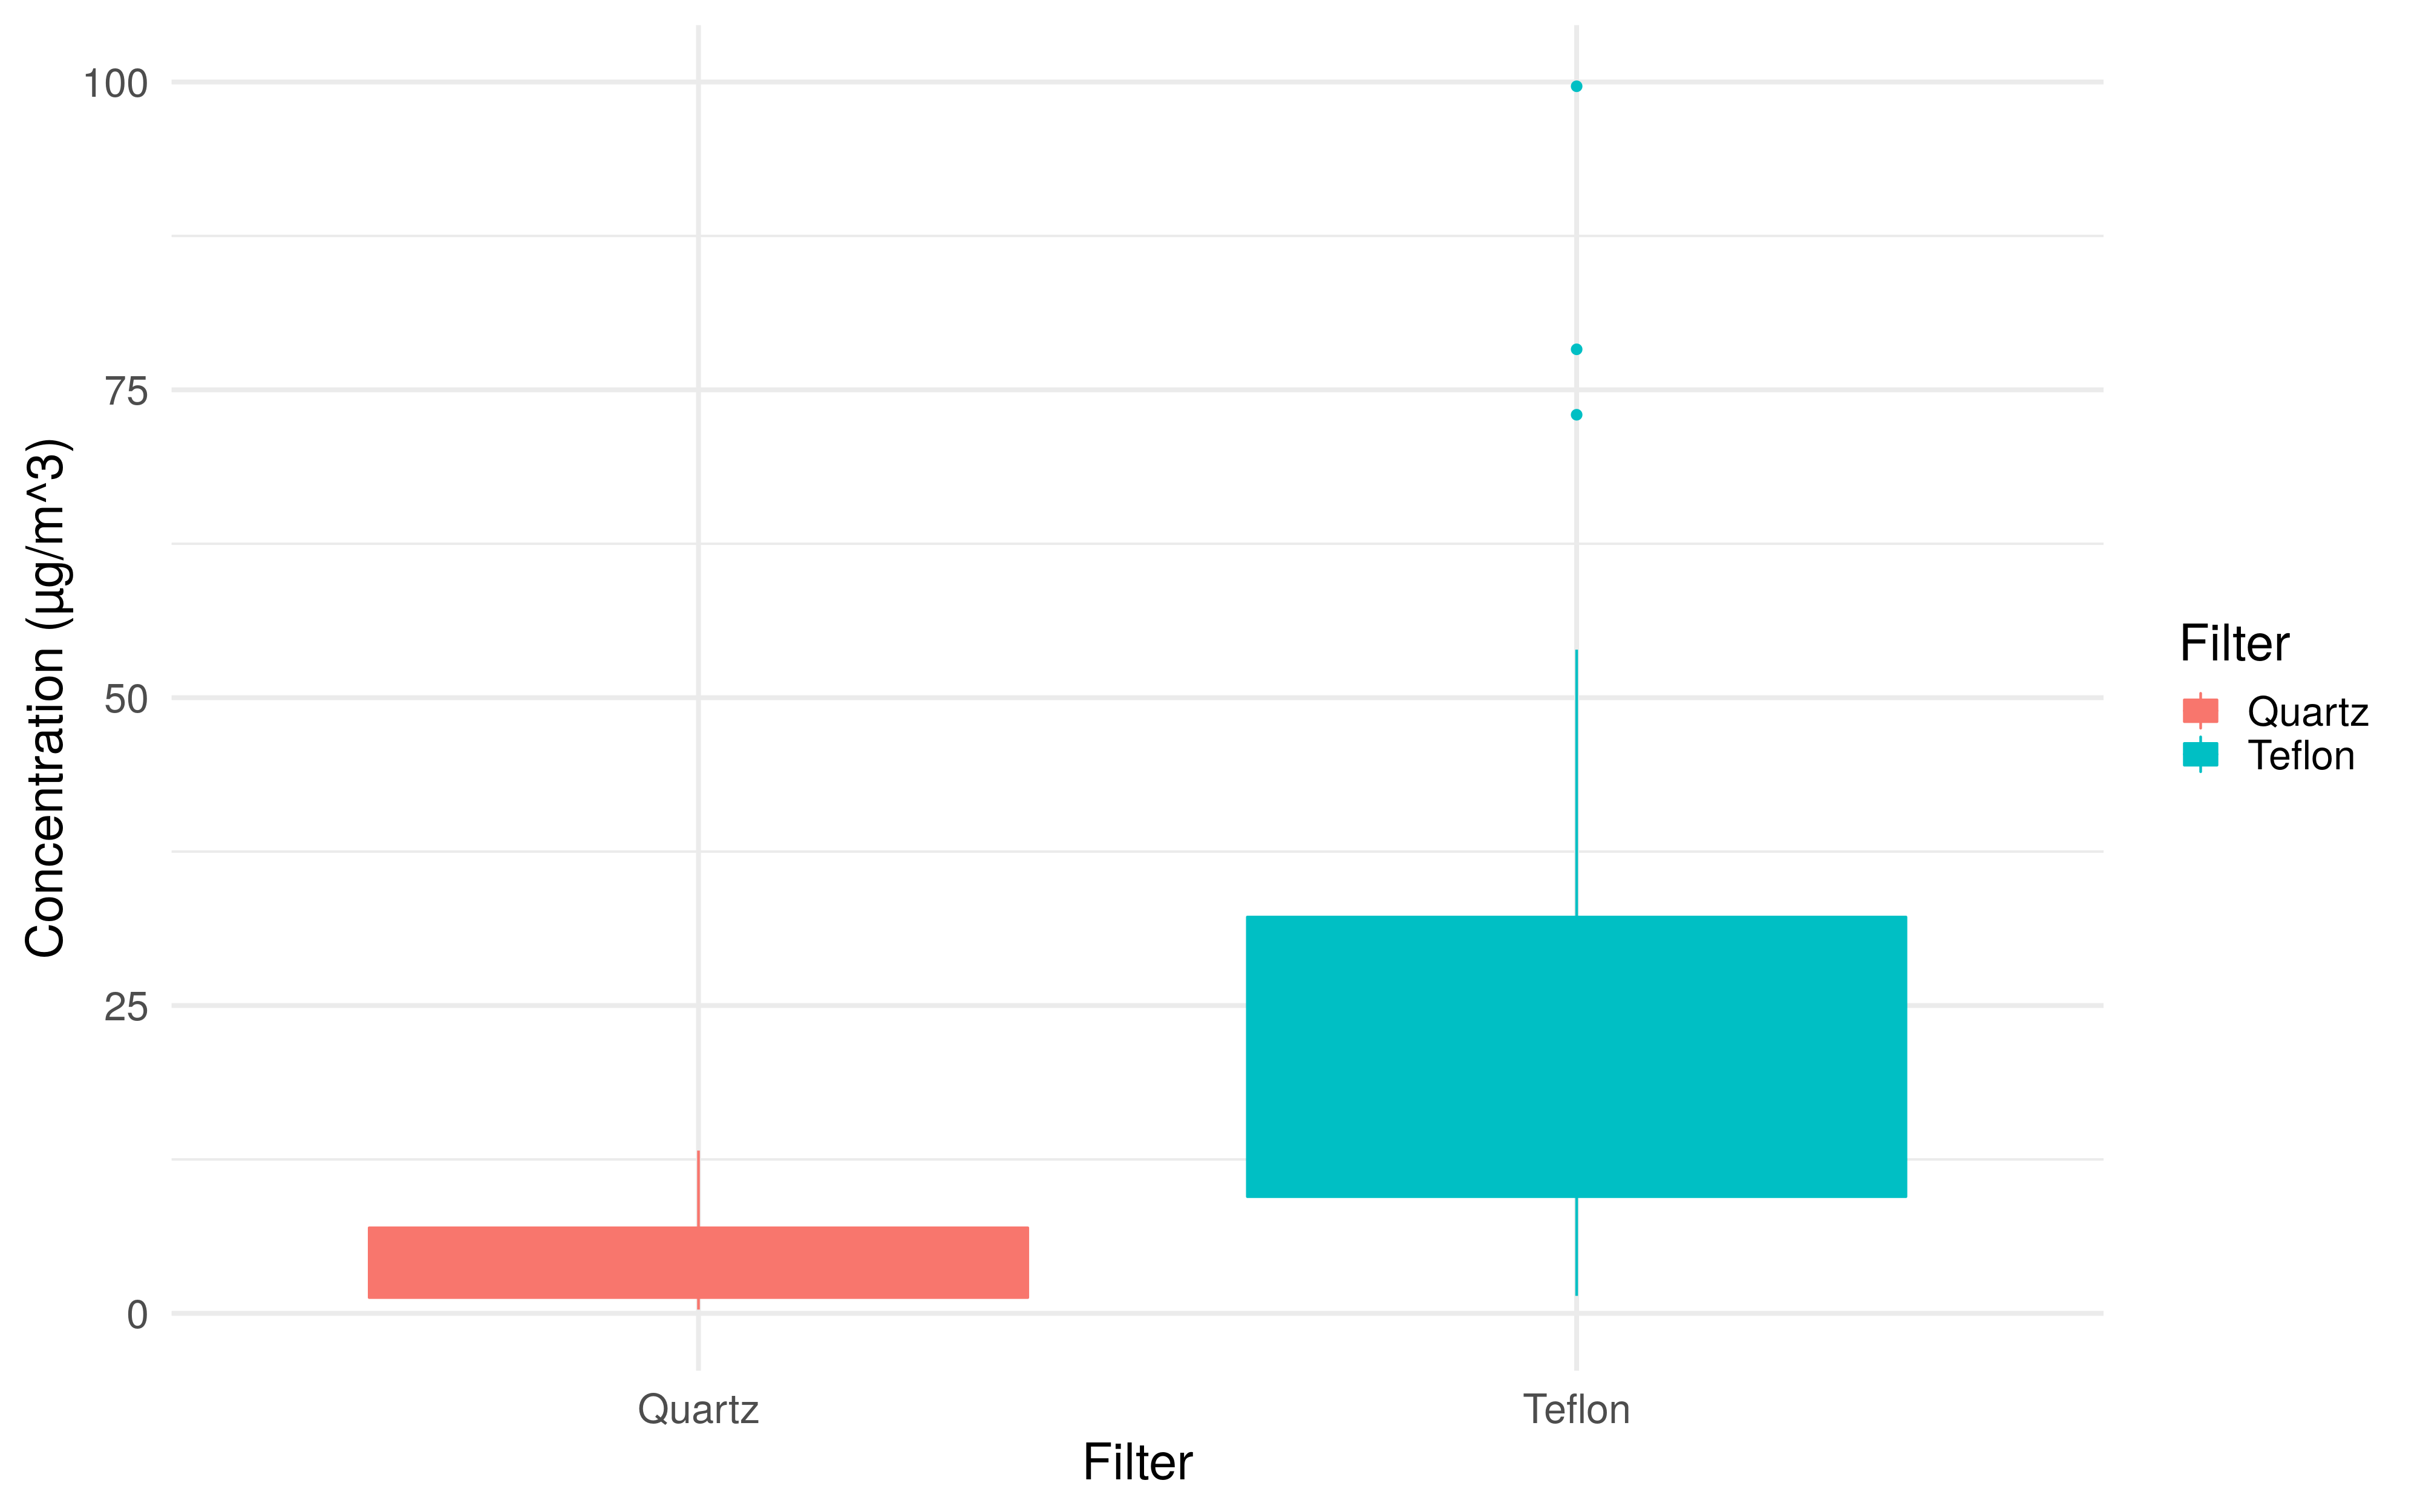
\includegraphics[width=\textwidth]{images/pm10_autumn_box_filter.png}
    \caption{Caption}
    \label{fig:pm10_autumn_box}
\end{figure}

What have we been doing so far

%%%%%%%%%%%%%%%%%%%%%%%%%%%%%%%%%%%%%%%%%%%%%%%%%%%%%%%%%%%%%

\chapter{Source apportionment campaigns}

Describe the campaigns and list data collected

%%%%%%%%%%%%%%%%%%%%%%%%%%%%%%%%%%%%%%%%%%%%%%%%%%%%%%%%%%%%%

\chapter{Conclusions}

What is the next step of the project 

\section{Next steps}

\section{Potential problems}

%%%%%%%%%%%%%%%%%%%%%%%%%%%%%%%%%%%%%%%%%%%%%%%%%%%%%%%%%%%%%

\begin{spacing}{0.3}
\linespread{0.8} \normalsize
\bibliography{library}
\end{spacing}

\end{document}
